\documentclass[a4paper, twoside, 12pt, openright]{report} % 'openright' assegura que cada capítol comença en una plana senar

\usepackage{booktabs}
\usepackage{verbatim} % Comentaris multilínea
\usepackage{graphicx} % Per insertar imatges
\usepackage{float} % Posicionament d'imatges
\usepackage{xcolor} % Colors per a blocs de codi
\usepackage{listings} % Blocs de codi i manifests YAML
\usepackage{microtype} % Micro-tipografia: millora justificació i evita overfull hbox

\usepackage[spanish]{babel} % Idioma
\usepackage{fancyhdr} % Per personalitzar capçaleres i peus de pàgina
\usepackage{etoolbox} % Per canviar estils de numeració
\usepackage{geometry} % Per ajustar marges
%\usepackage{emptypage} % Per evitar capçaleres/peus a pàgines en blanc
\usepackage{hyperref} % Afegeix glossari a la taula de continguts
\usepackage{setspace} % Per ajustar l'interlineat
\usepackage{titlesec} % Paquet per personalitzar els títols
\usepackage{newtxtext,newtxmath} % Paquet per fonts Times New Roman
\usepackage[nottoc, numbib]{tocbibind} % Inclou bibliografia i índexs automàticament al ToC
\usepackage[nonumberlist, toc]{glossaries} % Paquet per a la generació del glossari
\usepackage[style=ieee, backend=biber]{biblatex} % Paquet per gestionar la bibliografia en format IEEE
\addbibresource{references.bib} % El fitxer .bib amb les referències

% Carregar les definicions del glossari des d'un fitxer extern
\newglossaryentry{api_rest}{
    name={API REST},
    description={Interfaz de Programación de Aplicaciones basada en el paradigma \textit{Representational State Transfer} (REST), que utiliza el protocolo HTTP para facilitar la comunicación entre sistemas y permite realizar operaciones como consultar, crear, modificar y eliminar recursos de manera escalable y eficiente}
}

\newglossaryentry{gitops}{
    name={GitOps},
    description={Paradigma operativo que utiliza repositorios Git como fuente única de verdad para definir y gestionar el estado deseado de la infraestructura y las aplicaciones. Cualquier cambio en el sistema se realiza mediante commits en el repositorio, y un operador automatizado (como ArgoCD) se encarga de sincronizar el estado real del entorno con el estado declarado en Git}
}

\newglossaryentry{cni}{
    name={CNI},
    description={(\textit{Container Network Interface}) Especificación y conjunto de bibliotecas que definen cómo los plugins de red deben configurar las interfaces de red de los contenedores en Kubernetes. Ejemplos de plugins CNI son Calico, Flannel y Cilium}
}

\newglossaryentry{drift_protection}{
    name={Drift protection},
    description={Mecanismo que detecta y corrige automáticamente cualquier desviación entre el estado deseado de un recurso (definido declarativamente) y su estado real en el sistema. En el contexto de Kyverno, se implementa mediante el campo \texttt{synchronize: true} en las políticas de tipo \textit{generate}, que regenera automáticamente los recursos eliminados o modificados de forma no autorizada}
}

\newglossaryentry{auto_hardening}{
    name={Auto-hardening},
    description={Proceso automático de aplicación de configuraciones de seguridad sobre recursos del sistema sin intervención manual del operador o desarrollador. En el contexto de este trabajo, se implementa mediante políticas de mutación de Kyverno que inyectan campos de seguridad en los manifiestos de Kubernetes en el momento del despliegue}
}

\newglossaryentry{imds}{
    name={IMDS},
    description={(\textit{Instance Metadata Service}) Servicio disponible en entornos cloud (AWS, GCP, Azure) accesible desde cualquier instancia a través de la IP de enlace local \texttt{169.254.169.254}. Expone información sensible de la instancia como credenciales IAM temporales, tokens de servicio y configuración de red. Es un vector de ataque habitual en entornos de contenedores comprometidos}
}

\newglossaryentry{supply_chain_attack}{
    name={Ataque a la cadena de suministro},
    description={Tipo de ataque que compromete el software o las herramientas utilizadas durante el proceso de desarrollo o despliegue, en lugar de atacar directamente el sistema objetivo. En entornos CI/CD, puede manifestarse como la manipulación de dependencias, imágenes de contenedores, actions de GitHub o runners de terceros para inyectar código malicioso en el pipeline}
}

\newglossaryentry{policy_report}{
    name={PolicyReport},
    description={Recurso nativo de Kubernetes generado automáticamente por Kyverno que consolida los resultados de la evaluación de políticas sobre los recursos del clúster. Indica qué recursos han pasado, fallado o sido mutados por cada política, con marca temporal de cada evaluación. Existen dos variantes: \texttt{PolicyReport} (con alcance de namespace) y \texttt{ClusterPolicyReport} (con alcance de clúster)}
}

\newglossaryentry{webhook}{
    name={Webhook},
    description={Mecanismo de extensión del API Server de Kubernetes que permite invocar servicios HTTP externos durante el proceso de admisión de recursos. En el contexto de Kyverno, los webhooks de admisión son el canal por el que el API Server delega la evaluación de políticas al motor de Kyverno. Existen dos tipos: \texttt{MutatingWebhookConfiguration} (para políticas de mutación) y \texttt{ValidatingWebhookConfiguration} (para políticas de validación)}
}

\newglossaryentry{etcd}{
    name={etcd},
    description={Base de datos distribuida de tipo clave-valor que actúa como almacén persistente del estado completo del clúster Kubernetes. Todos los objetos del clúster (pods, services, configmaps, políticas, etc.) son persistidos en etcd una vez superado el proceso de admisión. Su consistencia y disponibilidad son críticas para el funcionamiento del clúster}
}

\newglossaryentry{hardening}{
    name={Hardening},
    description={Proceso de reducción de la superficie de ataque de un sistema mediante la eliminación o configuración restrictiva de funcionalidades innecesarias. En el contexto de contenedores Kubernetes, incluye medidas como desactivar la escalada de privilegios, eliminar Linux capabilities no requeridas, forzar la ejecución como usuario no root y restringir el acceso al sistema de ficheros}
}

\newglossaryentry{cidr}{
    name={CIDR},
    description={(\textit{Classless Inter-Domain Routing}) Notación utilizada para definir rangos de direcciones IP. En Kubernetes, los rangos CIDR se utilizan para designar el espacio de direccionamiento de los pods (pod CIDR) y de los servicios (service CIDR). Por ejemplo, \texttt{10.244.0.0/16} define el rango de IPs asignables a los pods cuando se utiliza Calico como plugin CNI}
}

\newglossaryentry{two_repo_gitops}{
    name={Patrón de dos repositorios (GitOps)},
    description={Patrón arquitectónico de GitOps que separa el repositorio de código fuente de la aplicación del repositorio de configuración que contiene los manifiestos de Kubernetes. El pipeline de CI actualiza el repositorio de configuración tras una build exitosa, y ArgoCD sincroniza el clúster con el estado declarado en dicho repositorio. Esta separación mejora la seguridad al limitar los permisos de acceso al clúster y clarifica las responsabilidades de cada componente}
}

\newglossaryentry{qos_kubernetes}{
    name={QoS (Kubernetes)},
    description={(\textit{Quality of Service}) Clasificación que Kubernetes asigna a los pods en función de cómo están definidos sus \texttt{resources.requests} y \texttt{resources.limits}. Existen tres clases: \texttt{Guaranteed} (requests == limits en todos los contenedores — máxima protección frente a evicción), \texttt{Burstable} (requests < limits o solo uno de los dos definido) y \texttt{BestEffort} (ningún campo definido — primera clase en ser eviccionada bajo presión de recursos)}
}

\newglossaryentry{patchstrategicmerge}{
    name={patchStrategicMerge},
    description={Mecanismo de aplicación de parches de Kyverno que realiza una fusión inteligente (\textit{merge}) del objeto Kubernetes original con el parche definido en la política. A diferencia de un reemplazo completo, \texttt{patchStrategicMerge} añade únicamente los campos ausentes y respeta los valores ya declarados explícitamente en el manifiesto original, garantizando que las mutaciones son aditivas y no destructivas}
}

\newglossaryentry{runner}{
    name={Runner (GitHub Actions)},
    description={Agente de ejecución que procesa los jobs definidos en los workflows de GitHub Actions. Puede ser un runner hospedado por GitHub (\textit{hosted runner}) o un runner autogestionado en infraestructura propia (\textit{self-hosted runner}). Los runners ejecutan cada paso del pipeline en un entorno aislado y son el objetivo de ataques de tipo supply chain que buscan comprometer el proceso de build o exfiltrar credenciales del entorno de CI}
}

\newglossaryentry{multi_tenant}{
    name={Multi-tenant},
    description={Modelo de despliegue de Kubernetes en el que un único clúster es compartido por múltiples equipos, aplicaciones o clientes (denominados \textit{tenants}) con aislamiento lógico mediante namespaces, RBAC y Network Policies. Este modelo optimiza el uso de recursos pero introduce desafíos de seguridad relacionados con el aislamiento entre \textit{tenants}, especialmente en escenarios donde un compromiso en una carga de trabajo podría propagarse a otras}
}


% Aplicar l'estil personalitzat
\setglossarystyle{altlist}
\setacronymstyle{long-short}

\makeglossaries

% ── Estil per a blocs de codi, comandes i manifests YAML ────────────────────
\definecolor{codbg}{RGB}{247,247,247}
\definecolor{codborder}{RGB}{210,210,210}
\lstdefinestyle{tfmcode}{
  backgroundcolor  = \color{codbg},
  basicstyle       = \ttfamily\small,
  breaklines       = true,
  breakatwhitespace= false,
  postbreak        = \mbox{{\footnotesize$\hookrightarrow$}\space},
  frame            = single,
  rulecolor        = \color{codborder},
  framesep         = 5pt,
  xleftmargin      = 8pt,
  xrightmargin     = 8pt,
  keepspaces       = true,
  columns          = flexible,
  showstringspaces = false,
  tabsize          = 2,
  aboveskip        = 4pt,
  belowskip        = 4pt,
  literate =
    {á}{{\'{a}}}1 {é}{{\'{e}}}1 {í}{{\'{i}}}1 {ó}{{\'{o}}}1 {ú}{{\'{u}}}1
    {Á}{{\'{A}}}1 {É}{{\'{E}}}1 {Í}{{\'{I}}}1 {Ó}{{\'{O}}}1 {Ú}{{\'{U}}}1
    {ñ}{{\~{n}}}1 {Ñ}{{\~{N}}}1
}
\lstset{style=tfmcode}
% ────────────────────────────────────────────────────────────────────────────

% Reduir espai abans i després de cada capítol
\titleformat{\chapter}[block]{\normalfont\fontsize{18pt}{0pt}\bfseries}{\thechapter}{1em}{}
\titlespacing*{\chapter}{0pt}{0pt}{\baselineskip}
\titlespacing*{\section}{0pt}{1.5ex plus .2ex}{0.8ex}
\titlespacing*{\subsection}{0pt}{1.5ex plus .2ex}{0.8ex}

\titleformat{\section}[block]{\normalfont\fontsize{16pt}{0pt}\bfseries}{\thesection}{1em}{}
\titleformat{\subsection}[block]{\normalfont\fontsize{14pt}{0pt}\bfseries}{\thesubsection}{1em}{}

\hypersetup{
    colorlinks=true,
    linkcolor=black,
    citecolor=black,
    filecolor=magenta,      
    urlcolor=blue,
    pdftitle={Títol TFG},
    pdfauthor={Nom alumne},
    pdfpagemode=FullScreen
}

% Configuració dels marges
\geometry{top=3cm, bottom=2.54cm, left=2.54cm, right=2.54cm, bindingoffset=0.46cm}

\setlength{\headheight}{14.5pt} % Augmentar l'altura de la capçalera

\setlength{\parindent}{0pt} % Desactiva el sagnat dels paràgrafs

% Definir carpeta d'imatges
\graphicspath{{images/}}

% Configuració de capçaleres i peus de pàgina preliminars
\fancypagestyle{plain}{
    \fancyhf{} % Esborrem configuracions prèvies
    \fancyhead[RO,LE]{\fontsize{10}{12}\textit{\thepage}}
    \fancyhead[RE]{\fontsize{10}{12}\textit{TFM}}
    \fancyfoot{}
}
\pagestyle{plain}

\title{
    \begin{center}
        \begin{minipage}{0.45\linewidth}
            \centering
            
\includegraphics[width=0.7\linewidth]{images/logo-tecnocampus.png}
        \end{minipage}
        \hfill
        \begin{minipage}{0.45\linewidth}
            \centering
            
\includegraphics[width=0.35\linewidth]{images/logo-udg.png}
        \end{minipage}

        \vspace{1.5cm}

        {\fontsize{14pt}{0pt}\textbf{Seguridad informática aplicada a Entornos industriales}} \\[1cm]

        \textbf{Diseño e implementación de una arquitectura DevSecOps basada en GitOps:}\\
        \textbf{Aseguramiento de la cadena de suministro en Kubernetes mediante scanners, ArgoCD y Kyverno} \\[1.5cm]

        \textbf{Memòria} \\[5cm]
    \end{center}
}
\author{
\fontsize{14pt}{0pt}
\textbf{Ziad El Karrabi El Hanafi} \\
\textbf{Tutor: Josep Andreu}
}
\date{2026}

\fontsize{12pt}{0pt}
\begin{document}

\maketitle

\newpage
\thispagestyle{empty} % Pàgina en blanc sense capçalera ni peu
\null
\newpage

% Estils dels índexs i numeració en xifres romanes
\pagenumbering{Roman} % Índexs comencen amb números romans

\tableofcontents


% Portada o altres planes sense numeració
\listoffigures

\listoftables

% Definir interlineat de 1,5 espais i espaiat anterior de 12pt
\onehalfspacing % Interlineat de 1,5
\setlength{\parskip}{12pt} % Espaiat anterior als paràgrafs

% Configuració de capçaleres i peus de pàgina principals
\fancypagestyle{plain}{
    \fancyhf{} % Esborrem configuracions prèvies
    \fancyhead[RO,LE]{\fontsize{10}{12}\textit{\thepage}}
    \fancyhead[LO]{\fontsize{10}{12}\textit{\nouppercase{\textit{\leftmark}}}}
    \fancyhead[RE]{\fontsize{10}{12}\textit{TFM}}
    \fancyfoot{}
}
\pagestyle{plain}
% Canvi a numeració aràbiga per al cos principal del document
\pagenumbering{arabic} % Comença numeració aràbiga
\chapter{Introducción}

La adopción de arquitecturas basadas en contenedores y orquestadores como Kubernetes ha transformado la forma en que se desarrollan y despliegan aplicaciones en entornos cloud y corporativos. Este paradigma permite automatizar la gestión del ciclo de vida de las aplicaciones, mejorar la escalabilidad y facilitar la integración de prácticas de desarrollo modernas. Sin embargo, esta evolución tecnológica también introduce nuevos desafíos en materia de seguridad, especialmente en entornos donde los despliegues se realizan de forma automatizada y continua.

En este contexto surge el enfoque DevSecOps, cuyo objetivo es integrar la seguridad dentro del propio ciclo de vida del desarrollo de software, en lugar de tratarla como una fase posterior al despliegue. Este modelo promueve la automatización de controles de seguridad dentro de los pipelines de integración y despliegue continuo, permitiendo detectar vulnerabilidades, aplicar políticas de seguridad y garantizar configuraciones seguras desde las primeras fases del desarrollo.

El presente Trabajo de Fin de Máster se centra en la implementación de un entorno DevSecOps completo sobre Kubernetes, integrando herramientas de Integración Continua (GitHub Actions) con análisis automatizado de vulnerabilidades mediante herramientas como Trivy y Sysdig Secure. Asimismo, se implementará un modelo de Despliegue Continuo basado en GitOps utilizando ArgoCD, permitiendo gestionar la infraestructura y los despliegues de forma declarativa a través de repositorios Git.

Adicionalmente, se incorporará el uso de Kyverno como motor de políticas de seguridad basado en Policy-as-Code, permitiendo aplicar controles automáticos sobre los manifiestos de Kubernetes durante el proceso de despliegue.

El núcleo del proyecto se basa en el uso de Admission Controllers, concretamente Kyverno, para aplicar políticas de seguridad de forma declarativa dentro del clúster de Kubernetes. A diferencia de los enfoques tradicionales que únicamente bloquean configuraciones inseguras, este trabajo explorará el uso de políticas de tipo mutating, capaces de corregir automáticamente configuraciones inseguras en los manifiestos YAML en tiempo de despliegue.

Finalmente, el proyecto incluirá un análisis comparativo entre Kyverno y OPA Gatekeeper, evaluando sus capacidades en la implementación de políticas de seguridad en Kubernetes, su facilidad de uso, curva de aprendizaje y eficacia en entornos de producción.

La Figura \ref{fig:arquitectura-devsecops} muestra una visión general de la arquitectura DevSecOps implementada en este trabajo, donde se integran los procesos de desarrollo, análisis de seguridad, despliegue continuo y aplicación de políticas dentro de un entorno Kubernetes.

\begin{figure}[H]
\centering
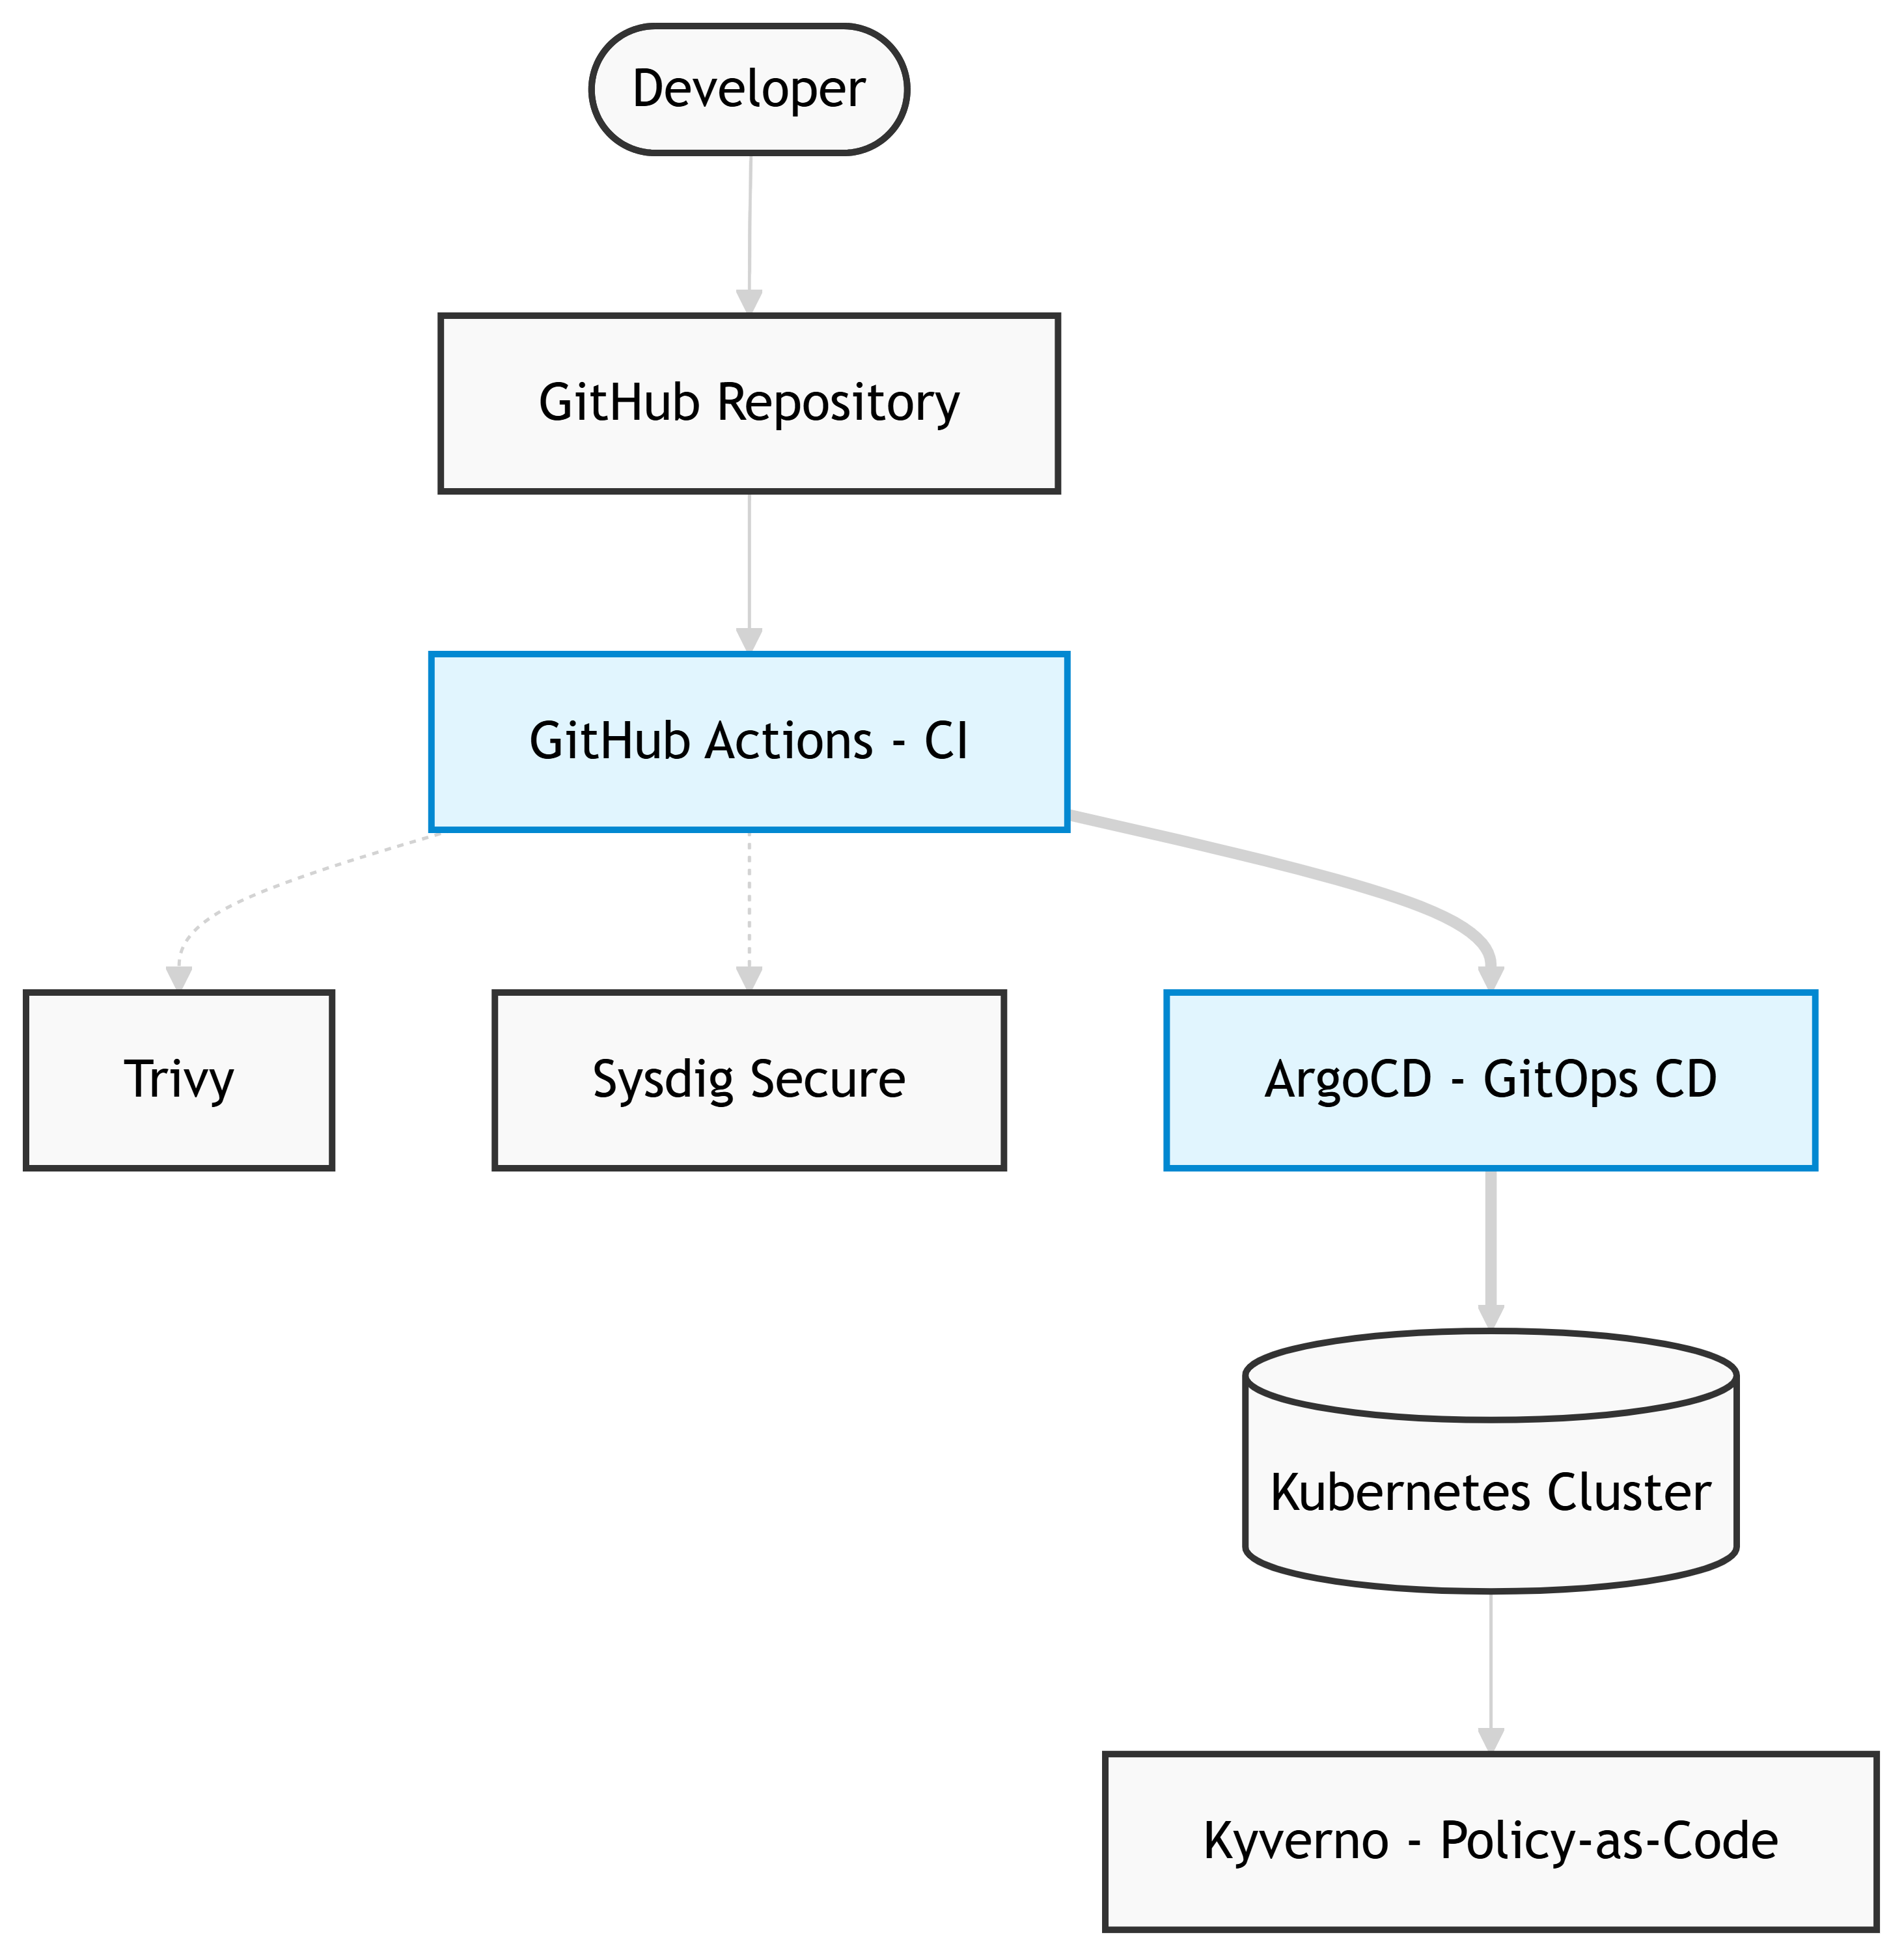
\includegraphics[width=0.5\linewidth]{images/arquitectura_DevSecOps.png}
\caption{Arquitectura general del entorno DevSecOps}
\label{fig:arquitectura-devsecops}
\end{figure}

\chapter{Marco teórico y análisis de referentes}

\section{Evolución del paradigma DevOps a DevSecOps}

\subsection{Limitaciones de los modelos tradicionales}

Los modelos tradicionales de desarrollo de software, como el modelo en cascada, se caracterizan por una separación estricta de fases (análisis, desarrollo, pruebas y despliegue), lo que dificulta la detección temprana de errores y vulnerabilidades \cite{pressman2019software}. En estos enfoques, la seguridad se introduce habitualmente en etapas finales, incrementando significativamente el coste de corrección y el riesgo en producción.

La adopción de metodologías ágiles y, posteriormente, del paradigma DevOps permitió mejorar la colaboración entre equipos y acelerar los ciclos de entrega \cite{kim2016devops}. Sin embargo, diversos estudios destacan que la seguridad continuó tratándose como un proceso independiente, generando vulnerabilidades especialmente en entornos cloud-native \cite{sharma2020devsecops}.

En este contexto, se hace evidente la necesidad de integrar mecanismos de seguridad automatizados que puedan aplicarse de forma continua dentro del ciclo de vida del software.

\subsection{Integración de la seguridad en el ciclo de vida del software}

La evolución hacia DevSecOps implica la integración de la seguridad desde las primeras fases del desarrollo, incorporando controles automatizados en pipelines CI/CD \cite{behl2017devsecops}. Esto incluye análisis de vulnerabilidades, validación de configuraciones y control de cumplimiento.

La automatización permite garantizar consistencia y reducir errores humanos, especialmente en entornos dinámicos. Según \cite{rahman2019devsecops}, la integración temprana de la seguridad mejora significativamente la resiliencia del software.

Este enfoque resulta clave en el presente trabajo, donde la seguridad se implementa mediante mecanismos automatizados integrados en Kubernetes.

\subsection{Nacimiento del concepto DevSecOps}

DevSecOps surge como una evolución natural de DevOps, integrando la seguridad como un componente intrínseco del ciclo de vida del software \cite{mohan2016towards}. Este paradigma promueve la automatización de controles de seguridad y la responsabilidad compartida entre equipos.

En entornos basados en contenedores y Kubernetes, este enfoque requiere mecanismos capaces de aplicar políticas de seguridad de forma dinámica y escalable.

En este trabajo, este objetivo se materializa mediante el uso de Policy-as-Code y herramientas como Kyverno, que permiten aplicar seguridad de forma declarativa y automatizada.

\section{Kubernetes como plataforma de ejecución}

\subsection{Arquitectura de Kubernetes}

Kubernetes se ha consolidado como el estándar de facto para la orquestación de contenedores, proporcionando una plataforma robusta para la gestión de aplicaciones distribuidas \cite{burns2016borg}.

Su arquitectura se basa en un plano de control (control plane), que gestiona el estado del sistema, y nodos worker encargados de ejecutar las cargas de trabajo. El API Server actúa como punto central de interacción mediante un modelo declarativo \cite{kubernetes_docs}.

Esta arquitectura permite automatizar la gestión del sistema, pero también introduce nuevos retos de seguridad que deben ser abordados mediante mecanismos específicos.

\subsection{Componentes principales del clúster}

Los componentes principales del control plane incluyen el API Server, el Scheduler y el Controller Manager, responsables de procesar solicitudes y mantener el estado deseado del sistema. En los nodos worker, el kubelet y el runtime de contenedores permiten la ejecución de los pods \cite{kubernetes_docs}.

La existencia de múltiples componentes distribuidos hace necesario implementar controles de seguridad centralizados, como los Admission Controllers.

\subsection{Gestión de red y Network Policies}

Por defecto, Kubernetes permite la comunicación libre entre pods, lo que puede representar un riesgo significativo. Las Network Policies permiten definir reglas de comunicación basadas en etiquetas y namespaces, aplicando el principio de mínimo privilegio \cite{kubernetes_docs}.

Además, en entornos reales es habitual encontrar configuraciones inseguras como:

\begin{itemize}
\item Contenedores ejecutándose como usuario root
\item Escalada de privilegios habilitada
\item Falta de límites de recursos
\item Acceso no restringido a red
\end{itemize}

Estas prácticas suponen un riesgo elevado, especialmente en entornos multi-tenant.

Esto justifica la necesidad de aplicar controles automáticos en el momento del despliegue mediante políticas de seguridad en Kubernetes.

\section{Policy-as-Code y Admission Controllers}

\subsection{Funcionamiento de los Admission Controllers}

Los Admission Controllers son mecanismos del API Server que interceptan las solicitudes antes de que los recursos sean persistidos en el clúster \cite{kubernetes_docs}. Permiten aplicar validaciones o modificaciones sobre los objetos.

Este mecanismo constituye la base técnica sobre la que se implementará la seguridad en este trabajo.

\subsection{Validación vs mutación de recursos}

Los \textit{validating admission controllers} permiten verificar que los recursos cumplen ciertas políticas, rechazando aquellos que no las satisfacen.

Por otro lado, los \textit{mutating admission controllers} permiten modificar automáticamente los recursos antes de su creación, aplicando configuraciones seguras por defecto.

En este trabajo se dará especial importancia a las políticas de tipo \textit{mutating}, ya que permiten aplicar mecanismos de hardening automático sobre los manifiestos, corrigiendo configuraciones inseguras sin intervención del usuario.

Este enfoque resulta clave para garantizar la seguridad en entornos DevSecOps altamente automatizados.

\subsection{Importancia de la seguridad declarativa}

El enfoque Policy-as-Code permite definir políticas de seguridad como código versionado, facilitando su integración en flujos GitOps \cite{huttermann2022devops}.

Este modelo mejora la trazabilidad, reproducibilidad y automatización de la seguridad.

En este trabajo, estos mecanismos serán implementados mediante Kyverno para aplicar políticas automáticamente en tiempo de despliegue.

\section{Herramientas y tecnologías utilizadas}

\subsection{Kyverno}

Kyverno es una herramienta de Policy-as-Code diseñada específicamente para Kubernetes que permite definir políticas utilizando YAML, sin necesidad de aprender lenguajes adicionales \cite{kyverno_docs}.

A diferencia de otras soluciones, Kyverno permite definir políticas directamente en el mismo formato utilizado por Kubernetes, lo que facilita su adopción. Además, soporta tanto políticas de validación como de mutación, permitiendo no solo bloquear configuraciones inseguras, sino también corregirlas automáticamente.

Esta capacidad resulta especialmente relevante en entornos DevSecOps, donde la automatización y la consistencia son factores clave.

Kyverno constituye el eje central de este trabajo.

\subsection{OPA Gatekeeper}

Open Policy Agent (OPA) es un motor de políticas generalista que permite definir reglas mediante el lenguaje Rego \cite{opa_docs}. Gatekeeper facilita su integración con Kubernetes.

Aunque ofrece gran flexibilidad, su complejidad y enfoque basado en validación lo diferencian de Kyverno.

\subsection{ArgoCD y GitOps}

ArgoCD implementa el paradigma GitOps, donde el estado del sistema se define en repositorios Git \cite{weaveworks_gitops}.

En este trabajo, se utilizará para automatizar el despliegue y garantizar la coherencia entre configuración y estado real.

\subsection{GitHub Actions}

GitHub Actions permite automatizar pipelines CI/CD, incluyendo procesos de build, test y seguridad \cite{github_actions_docs}.

Se utilizará para integrar controles de seguridad dentro del flujo DevSecOps.

\subsection{Trivy y Sysdig Secure}

Trivy permite el escaneo de vulnerabilidades en imágenes de contenedores \cite{trivy_docs}, mientras que Sysdig Secure proporciona seguridad en tiempo de ejecución \cite{sysdig_secure}.

Estas herramientas complementan la seguridad aplicada mediante políticas en Kubernetes.

\section{Comparativa teórica Kyverno vs OPA}

Las herramientas Kyverno y Open Policy Agent (OPA) representan dos de las soluciones más relevantes dentro del enfoque \textit{Policy-as-Code} aplicado a Kubernetes. Ambas permiten definir y aplicar políticas de seguridad sobre los recursos del clúster, aunque presentan diferencias significativas en cuanto a su diseño, enfoque y capacidades \cite{opa_docs, kyverno_docs}.

Kyverno es una herramienta diseñada específicamente para Kubernetes (\textit{Kubernetes-native}), que permite definir políticas utilizando el mismo formato YAML empleado en los manifiestos del propio sistema. Este enfoque reduce la complejidad y facilita su adopción por parte de equipos DevOps familiarizados con Kubernetes. Por el contrario, OPA utiliza el lenguaje Rego, un lenguaje declarativo de propósito general que ofrece una gran flexibilidad, pero introduce una mayor curva de aprendizaje.

Desde el punto de vista funcional, ambas herramientas permiten implementar políticas de validación (\textit{validating}), es decir, comprobar que los recursos cumplen determinadas condiciones antes de ser desplegados. Sin embargo, una diferencia clave radica en el soporte de políticas de mutación (\textit{mutating}). Kyverno permite modificar automáticamente los recursos en tiempo de admisión, aplicando configuraciones seguras por defecto, mientras que OPA Gatekeeper se centra principalmente en la validación, careciendo de soporte nativo para la mutación de recursos.

A continuación, se presenta una comparativa resumida de ambas herramientas:

\begin{table}[H]
\centering
\begin{tabular}{lcc}
\toprule
\textbf{Característica} & \textbf{Kyverno} & \textbf{OPA Gatekeeper} \\
\midrule
Enfoque & Kubernetes-native & Generalista \\
Lenguaje de políticas & YAML & Rego \\
Curva de aprendizaje & Baja & Alta \\
Validación de recursos & Sí & Sí \\
Mutación de recursos & Sí & No (limitada) \\
Integración con Kubernetes & Nativa & Mediante CRDs \\
Facilidad de adopción & Alta & Media \\
\bottomrule
\end{tabular}
\caption{Comparativa entre Kyverno y OPA Gatekeeper}
\label{tab:kyverno-vs-opa}
\end{table}


Estas diferencias tienen un impacto directo en su aplicabilidad en entornos DevSecOps. Mientras que OPA ofrece una mayor expresividad y flexibilidad para definir políticas complejas, Kyverno destaca por su simplicidad operativa y su capacidad de integrarse de forma natural en flujos de trabajo basados en Kubernetes.

Desde la perspectiva de este trabajo, la capacidad de mutación de Kyverno resulta especialmente relevante, ya que permite implementar mecanismos de \textit{hardening} automático sobre los manifiestos, corrigiendo configuraciones inseguras sin necesidad de intervención manual. Esto incluye, por ejemplo, la adición automática de límites de recursos, la desactivación de privilegios elevados o la aplicación de políticas de red por defecto.

En consecuencia, Kyverno se posiciona como una herramienta especialmente adecuada para entornos donde se prioriza la automatización, la consistencia y la integración con prácticas GitOps.

Esta comparativa teórica servirá como base para el análisis práctico que se desarrollará en capítulos posteriores, donde se evaluará el comportamiento de ambas soluciones en un entorno real de Kubernetes.


\chapter{Objetivos y alcance}

\section{Objetivo general}

El objetivo principal de este Trabajo de Fin de Máster es el diseño e implementación de un entorno funcional de DevSecOps sobre Kubernetes, integrando mecanismos de seguridad de forma nativa dentro del ciclo de vida del desarrollo y despliegue de aplicaciones.

El núcleo del proyecto se centra en la aplicación del paradigma Policy-as-Code mediante el uso de Admission Controllers, concretamente Kyverno, con el objetivo de garantizar configuraciones seguras en tiempo de despliegue. A diferencia de los enfoques tradicionales basados únicamente en la detección o el bloqueo, este trabajo pone especial énfasis en el uso de políticas de tipo \textit{mutating}, capaces de corregir automáticamente configuraciones inseguras en los manifiestos de Kubernetes.

Esta aproximación permite no solo prevenir errores de configuración, sino también establecer mecanismos de hardening automático, alineados con las prácticas modernas de seguridad en entornos cloud-native.

\section{Objetivos específicos}

Para alcanzar el objetivo general, se definen los siguientes objetivos específicos:

\begin{itemize}
    \item Desplegar un clúster Kubernetes funcional en un entorno de laboratorio, con una arquitectura basada en un nodo de control y un nodo worker, configurando adecuadamente su comunicación y la capa de red mediante una solución CNI como Calico.

    \item Instalar y configurar Kyverno como motor de políticas de seguridad basado en Policy-as-Code, integrándolo como Admission Controller dentro del clúster.

    \item Definir e implementar un conjunto representativo de políticas de seguridad (entre 5 y 10), centradas en problemáticas reales como:
    \begin{itemize}
        \item ejecución de contenedores con privilegios elevados,
        \item escalada de privilegios,
        \item ausencia de límites de recursos,
        \item control de comunicaciones de red.
    \end{itemize}

    \item Validar el comportamiento de las políticas mediante pruebas prácticas, demostrando tanto el bloqueo de configuraciones inseguras (\textit{validating policies}) como su corrección automática (\textit{mutating policies}).

    \item Implementar una política avanzada basada en la generación automática de Network Policies, con el objetivo de restringir accesos a recursos sensibles, como servicios de metadatos (por ejemplo, la IP 169.254.169.254), habitual en entornos cloud.

    \item Integrar el clúster dentro de un modelo de despliegue continuo basado en GitOps, utilizando ArgoCD para gestionar el estado declarativo de las aplicaciones.

    \item Incorporar un pipeline de integración continua mediante GitHub Actions, incluyendo procesos de construcción y análisis de vulnerabilidades con herramientas como Trivy o Sysdig Secure.

    \item Realizar una comparativa técnica entre Kyverno y OPA Gatekeeper, analizando diferencias en facilidad de uso, capacidades de validación y mutación, y adecuación en entornos productivos.
\end{itemize}

\section{Alcance del proyecto}

El proyecto se desarrolla en un entorno de laboratorio basado en máquinas virtuales, con el objetivo de reproducir un escenario realista de despliegue en Kubernetes. El alcance incluye la configuración del clúster, la integración de las herramientas principales del pipeline DevSecOps y la implementación de políticas de seguridad representativas.

No obstante, el trabajo no pretende cubrir de manera exhaustiva todos los estándares de seguridad existentes, sino demostrar el funcionamiento y la viabilidad del modelo Policy-as-Code aplicado a Kubernetes mediante casos prácticos.

Asimismo, la utilización de herramientas de automatización como Ansible se considera una posible ampliación del proyecto. Siguiendo un enfoque iterativo, se prioriza inicialmente la implementación de los mecanismos de seguridad y su validación, dejando la automatización completa del despliegue como una línea de trabajo futura o paralela en función del tiempo disponible.
\chapter{Metodología del proyecto}

El presente capítulo describe el enfoque metodológico adoptado para llevar a cabo el Trabajo de Fin de Máster. No se trata de un capítulo técnico, sino de una descripción razonada de cómo se ha planificado el trabajo, qué decisiones se han tomado respecto al alcance y la organización del proyecto, y qué criterios han guiado la selección de herramientas y la definición de las fases de desarrollo. Muchas de estas decisiones han sido consensuadas con el tutor, Josep Andreu, a lo largo de distintas reuniones y comunicaciones que han servido para ajustar progresivamente el enfoque del trabajo.

% ─────────────────────────────────────────────
\section{Enfoque general del proyecto}
% ─────────────────────────────────────────────

El proyecto adopta un enfoque de \textbf{investigación aplicada con desarrollo práctico}. El objetivo no es realizar una revisión teórica exhaustiva de los estándares de seguridad en Kubernetes, sino construir un entorno funcional real que demuestre cómo integrar la seguridad de forma automatizada dentro del ciclo de vida del desarrollo y el despliegue. Los resultados se validan empíricamente a través de pruebas controladas sobre el entorno implementado, no mediante análisis bibliográfico.

El tutor orientó el trabajo hacia un número manejable de entre cinco y diez políticas de seguridad bien elegidas, con el argumento de que demostrar el funcionamiento y la comprensión profunda de Kyverno es más valioso académicamente que aplicar un estándar completo de forma superficial. Esta directriz ha marcado toda la planificación del proyecto: se prioriza la calidad y la justificación de cada decisión sobre la cantidad de elementos implementados.

El desarrollo sigue un modelo \textbf{iterativo e incremental}: se comienza con los componentes más fundamentales (el clúster y Kyverno), se valida cada elemento antes de añadir el siguiente, y se avanza progresivamente hacia los componentes de mayor complejidad (ArgoCD, GitHub Actions, comparativa con OPA). Este modelo permite detectar problemas de integración de forma temprana y garantiza que el entorno es funcional en todo momento, incluso antes de estar completo.

% ─────────────────────────────────────────────
\section{Entorno de laboratorio}
% ─────────────────────────────────────────────

El entorno sobre el que se desarrolla el proyecto consiste en un clúster Kubernetes desplegado sobre dos máquinas virtuales proporcionadas por el tutor, gestionadas con VirtualBox. Esta decisión fue consensuada durante el intercambio inicial con Josep Andreu, quien recomendó utilizar las imágenes de las máquinas empleadas en la asignatura para garantizar coherencia y estabilidad.

Las dos máquinas virtuales tienen los siguientes roles y direcciones IP fijas dentro de la red del laboratorio:

\begin{itemize}
    \item \textbf{Nodo de control} (\textit{control plane}): \texttt{192.168.1.101}, hostname \texttt{control}. Aloja el plano de control de Kubernetes y actúa como punto de entrada para todas las operaciones de administración del clúster.
    \item \textbf{Nodo worker}: \texttt{192.168.1.102}, hostname \texttt{worker}. Ejecuta las cargas de trabajo desplegadas en el clúster.
\end{itemize}

Cada máquina virtual está configurada con dos interfaces de red: una de tipo NAT para el acceso a internet, y una de tipo \textit{Host-only Adapter} para la comunicación interna entre nodos. La capa de red del clúster se implementa mediante \textbf{Calico v3.28} \cite{calico_docs}, un plugin CNI que permite definir y aplicar efectivamente Network Policies, lo cual es un requisito para una de las políticas de seguridad implementadas en el proyecto.

La elección de un entorno virtualizado local, en lugar de un proveedor cloud, responde a criterios de control y reproducibilidad. No obstante, esta decisión tiene implicaciones sobre el alcance del trabajo, que se detallan al final de este capítulo.

% ─────────────────────────────────────────────
\section{Fases del proyecto}
% ─────────────────────────────────────────────

El proyecto se organiza en cinco fases secuenciales. Cada fase tiene un alcance delimitado y no se avanza a la siguiente hasta verificar que la anterior es funcional.

\subsection{Fase 1: Aprovisionamiento del clúster Kubernetes}

La primera fase comprende la puesta en marcha del clúster Kubernetes sobre las dos máquinas virtuales del laboratorio. Incluye la inicialización del nodo de control, la incorporación del nodo worker y la instalación del plugin de red Calico. El resultado esperado es un clúster operativo con ambos nodos activos y todos los componentes del sistema en funcionamiento.

\subsection{Fase 2: Despliegue e integración de Kyverno}

La segunda fase introduce Kyverno como motor de políticas de seguridad dentro del clúster. Kyverno se instala como un conjunto de controladores que se integran en el mecanismo de Admission Controllers de Kubernetes, interceptando las solicitudes al API Server para aplicar las políticas definidas. Esta fase también incluye la verificación de que los webhooks de Kyverno están correctamente registrados y operativos antes de proceder con la implementación de políticas.

\subsection{Fase 3: Implementación de políticas de seguridad}

La tercera fase constituye el núcleo del trabajo. Se diseña e implementa un conjunto de políticas de seguridad que cubren los tres tipos de acción disponibles en Kyverno: validación, mutación y generación. Las políticas se aplican de forma incremental, comenzando por las más simples (validación de configuraciones inseguras) y avanzando hacia las de mayor complejidad (mutación automática de manifiestos y generación de recursos derivados).

\subsection{Fase 4: Integración GitOps con ArgoCD}

Una vez que las políticas están validadas y operativas, la cuarta fase introduce ArgoCD para gestionar el estado del clúster de forma declarativa a través de un repositorio Git. Todas las configuraciones — políticas de Kyverno, manifiestos de prueba y configuraciones de infraestructura — se almacenan en Git, y ArgoCD garantiza que el estado del clúster se mantiene sincronizado con el repositorio. Esta fase demuestra el ciclo GitOps completo: cualquier cambio en el repositorio se propaga automáticamente al clúster, y cualquier desviación manual es detectada y revertida.

\subsection{Fase 5: Integración CI/CD con GitHub Actions y Trivy}

La quinta fase incorpora la dimensión de integración continua al entorno DevSecOps. Se configura un pipeline en GitHub Actions que ejecuta automáticamente un análisis de vulnerabilidades sobre las imágenes de contenedores utilizadas, empleando Trivy como motor de escaneo. Esta fase cierra el ciclo DevSecOps completo e introduce además la consideración de los riesgos de la propia cadena de suministro del pipeline, motivada por la alerta del tutor sobre el ataque del grupo TeamPCP, que comprometió pipelines CI/CD mediante la manipulación de actions y runners de terceros \cite{teampcp2026}.

% ─────────────────────────────────────────────
\section{Selección y alcance de las políticas de seguridad}
% ─────────────────────────────────────────────

El conjunto de políticas implementadas no pretende cubrir de forma exhaustiva todos los controles de seguridad existentes para Kubernetes. Siguiendo la orientación del tutor, se han seleccionado entre cinco y diez políticas que ilustran los diferentes mecanismos de acción de Kyverno y que corresponden a problemáticas de seguridad reales y bien documentadas.

Las políticas seleccionadas abordan las siguientes categorías de riesgo:

\begin{itemize}
    \item Ejecución de contenedores con el usuario root
    \item Escalada de privilegios en tiempo de ejecución
    \item Uso de imágenes procedentes de registros no autorizados
    \item Ausencia de límites de recursos (CPU y memoria)
    \item Configuración insegura del contexto de seguridad del contenedor
    \item Acceso de escritura al sistema de ficheros del contenedor
    \item Acceso al servicio de metadatos de instancia cloud (IP 169.254.169.254)
\end{itemize}

La última política — el bloqueo del acceso al servicio de metadatos cloud — fue propuesta explícitamente por el tutor como ejemplo ilustrativo del mecanismo de generación de Kyverno. Mediante una política de tipo \textit{generate}, Kyverno crea automáticamente una NetworkPolicy en cada namespace nuevo del clúster que impide el acceso a dicha IP. Si la NetworkPolicy es eliminada manualmente, Kyverno la regenera de forma automática, demostrando el concepto de protección frente a desviaciones de configuración (\textit{drift protection}).

Adicionalmente, el tutor señaló el interés de incorporar validación de imágenes mediante firma digital con herramientas como Cosign o Notary, así como el uso del contexto \texttt{imageRegistry} de Kyverno para inspeccionar metadatos de imágenes. Estas funcionalidades se contemplan como una posible ampliación del trabajo si el tiempo disponible lo permite, pero no forman parte del alcance comprometido.

% ─────────────────────────────────────────────
\section{Reporting y observabilidad del sistema}
% ─────────────────────────────────────────────

El tutor indicó expresamente que el reporting es un valor añadido relevante para el proyecto. Kyverno genera automáticamente recursos \texttt{PolicyReport} y \texttt{ClusterPolicyReport} que consolidan los resultados de la evaluación de políticas sobre todos los recursos del clúster. Estos informes permiten conocer, de forma centralizada, qué recursos cumplen cada política, cuáles han sido mutados automáticamente y cuáles han sido rechazados.

La revisión y documentación de estos informes forma parte del plan de validación del sistema y se incluirá como evidencia en el capítulo de resultados. Este mecanismo aporta una dimensión de auditoría y compliance que complementa las pruebas funcionales individuales y demuestra la aplicabilidad del sistema en entornos reales donde la trazabilidad de las evaluaciones de seguridad es un requisito.

% ─────────────────────────────────────────────
\section{Estrategia de validación}
% ─────────────────────────────────────────────

La validación del sistema se realiza mediante pruebas controladas sobre el entorno de laboratorio. Para cada política implementada se ejecuta al menos un escenario de prueba que demuestra su comportamiento con evidencia documental directa: salidas de comandos, estados del sistema y capturas del entorno.

Las pruebas se organizan en tres categorías:

\begin{itemize}
    \item \textbf{Pruebas de bloqueo}: se intenta desplegar un recurso que infringe una política de validación y se verifica que el API Server lo rechaza con el mensaje de error correspondiente.
    \item \textbf{Pruebas de mutación}: se despliega un recurso con una configuración incompleta o mínima y se comprueba que Kyverno ha aplicado automáticamente los campos de seguridad esperados, sin que el desarrollador haya tenido que especificarlos.
    \item \textbf{Pruebas de generación}: se crea un namespace y se verifica tanto la generación automática de la NetworkPolicy asociada como su regeneración tras un borrado manual, demostrando el mecanismo de \textit{drift protection}.
\end{itemize}

Adicionalmente, se ejecuta una prueba integral que despliega un pod con configuración mínima y verifica que el conjunto de políticas de mutación activas lo transforma en un pod con perfil de seguridad completo. Esta prueba constituye la demostración más representativa del concepto central del trabajo: el \textit{auto-hardening} automático y transparente para el desarrollador.

% ─────────────────────────────────────────────
\section{Comparativa con OPA Gatekeeper}
% ─────────────────────────────────────────────

El proyecto incluye una comparativa práctica entre Kyverno y OPA Gatekeeper. Para ello, se reimplementarán en OPA un subconjunto representativo de las políticas ya definidas en Kyverno, con el objetivo de ilustrar las diferencias en sintaxis, capacidades y facilidad de uso. La comparativa no busca determinar cuál herramienta es superior en términos absolutos, sino evaluar cuál se adapta mejor a las necesidades concretas de un entorno DevSecOps automatizado donde la mutación y la generación de recursos son requisitos clave.

Este ejercicio práctico complementa la comparativa teórica del capítulo 2 y permite extraer conclusiones fundamentadas en la experiencia directa con ambas herramientas.

% ─────────────────────────────────────────────
\section{Decisiones de alcance y limitaciones previstas}
% ─────────────────────────────────────────────

A lo largo del proceso de planificación, se han tomado varias decisiones explícitas sobre el alcance del proyecto que conviene documentar:

\textbf{Sysdig Secure.} El tutor advirtió que Sysdig Secure es un servicio SaaS que ha presentado históricamente problemas de integración con máquinas virtuales, requiriendo en ocasiones el uso de infraestructura cloud para funcionar correctamente. Se contempla su integración si resulta viable con el entorno de laboratorio, pero se acepta de antemano que puede ser necesario documentar la limitación y sustituirla por un análisis de las capacidades de seguridad en tiempo de ejecución que la herramienta ofrecería en un entorno cloud real.

\textbf{Ansible.} Aunque existe interés en incorporar Ansible para automatizar el provisionamiento del clúster y la instalación de los componentes, el tutor recomendó abordarlo únicamente si el resto del trabajo está completo. Ansible se contempla como una ampliación opcional que no condiciona la entrega principal del proyecto.

\textbf{Validación avanzada de imágenes.} Las funcionalidades de verificación de firmas digitales (Cosign, Notary) y de inspección de metadatos mediante \texttt{imageRegistry} quedan fuera del alcance comprometido, aunque se incluirán si el tiempo lo permite. Su ausencia no afecta a la demostración del modelo Policy-as-Code, que queda suficientemente cubierta por el conjunto de políticas principal.

Estas decisiones reflejan una planificación realista orientada a garantizar un entregable sólido dentro del tiempo disponible, en lugar de abarcar un alcance excesivo con riesgo de quedarse incompleto.

\chapter{Diseño de la arquitectura}

El presente capítulo describe el diseño arquitectónico del entorno DevSecOps implementado en este trabajo. Se expone la visión general del sistema, el papel de cada componente, el flujo completo de integración y despliegue continuo con seguridad integrada, la topología de red del clúster de laboratorio y, finalmente, las decisiones de diseño que han guiado la construcción del entorno y las razones técnicas que las justifican.

% ─────────────────────────────────────────────
\section{Arquitectura general del sistema}
% ─────────────────────────────────────────────

La arquitectura del sistema se organiza en tres planos funcionales claramente diferenciados: el plano de desarrollo, el plano de automatización y el plano de ejecución. Esta separación no es meramente conceptual, sino que refleja una división real de responsabilidades entre los componentes del sistema y los momentos del ciclo de vida en los que actúa cada uno.

El \textbf{plano de desarrollo} abarca el conjunto de actividades realizadas por el equipo de ingeniería: la escritura de código de aplicación, la definición de manifiestos Kubernetes y la formulación de políticas de seguridad. Toda esta producción se materializa en forma de commits sobre repositorios Git, que constituyen la fuente de verdad del sistema.

El \textbf{plano de automatización} comprende los mecanismos que procesan los cambios introducidos en los repositorios y transforman el código en artefactos desplegables, verificando su seguridad en el proceso. Este plano engloba el pipeline de integración continua gestionado por GitHub Actions, que construye las imágenes de contenedor y las somete a análisis de vulnerabilidades mediante Trivy, y el controlador GitOps implementado por ArgoCD, que detecta las diferencias entre el estado deseado definido en Git y el estado real del clúster y aplica las reconciliaciones necesarias.

El \textbf{plano de ejecución} corresponde al clúster Kubernetes, donde las cargas de trabajo finalmente se despliegan y donde Kyverno actúa como última línea de defensa, interceptando cada solicitud de creación o modificación de recursos para aplicar las políticas de seguridad definidas antes de que cualquier objeto sea persistido en el sistema.

La Figura~\ref{fig:arquitectura-general} ilustra la arquitectura global del sistema, mostrando la relación entre los tres planos y los flujos de información entre ellos.

\begin{figure}[H]
\centering
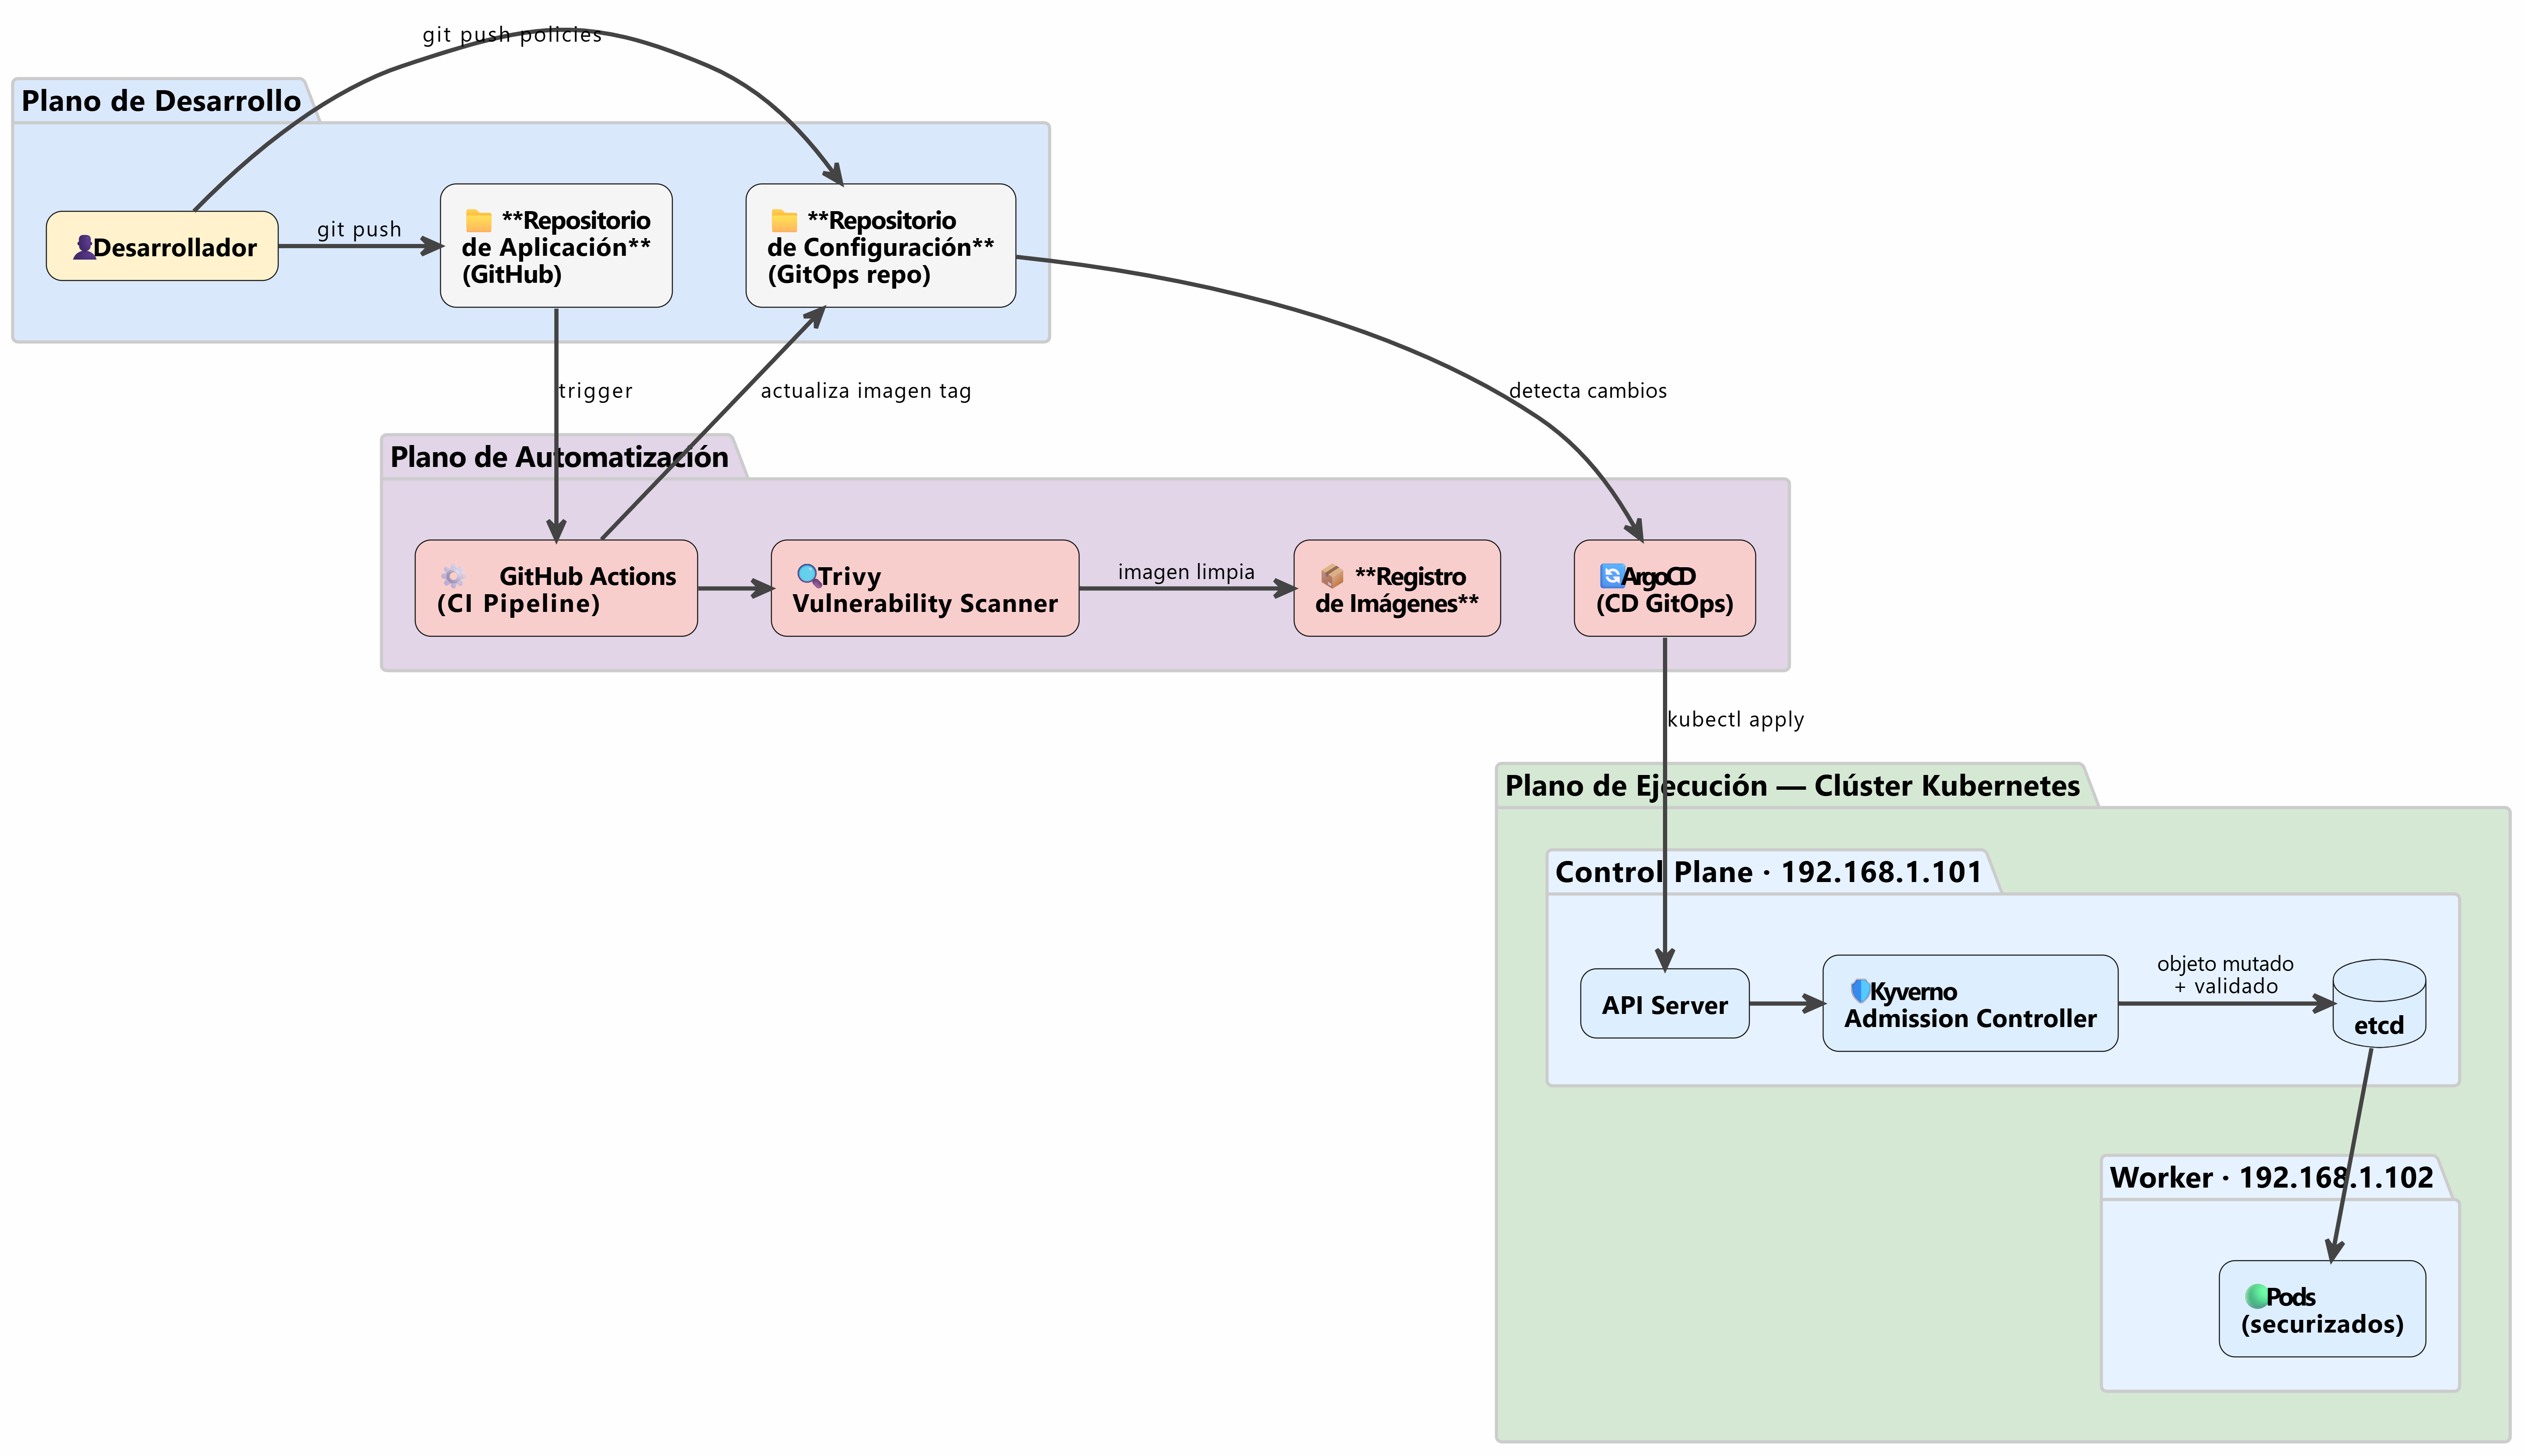
\includegraphics[width=0.95\linewidth]{arquitectura/fig5-1-arquitectura-general.png}
\caption{Arquitectura general del entorno DevSecOps}
\label{fig:arquitectura-general}
\end{figure}

Un aspecto arquitectónico central es la adopción del \textbf{patrón de dos repositorios} para la implementación del modelo GitOps. El repositorio de aplicación contiene el código fuente de las cargas de trabajo y la lógica de negocio, mientras que el repositorio de configuración —denominado habitualmente \textit{GitOps repo}— almacena los manifiestos de Kubernetes, las políticas de Kyverno y las configuraciones de infraestructura. Esta separación permite que el pipeline de CI modifique únicamente el repositorio de configuración (actualizando la etiqueta de imagen tras una build exitosa) sin que ArgoCD deba tener acceso al código fuente de la aplicación, reduciendo la superficie de ataque y clarificando las responsabilidades de cada componente.

% ─────────────────────────────────────────────
\section{Descripción de componentes}
% ─────────────────────────────────────────────

\subsection{Clúster Kubernetes}

El clúster Kubernetes constituye la plataforma de ejecución sobre la que se sustenta el conjunto del sistema. Siguiendo la arquitectura descrita en el Capítulo~4, se compone de dos nodos: un nodo de control (\texttt{192.168.1.101}) y un nodo worker (\texttt{192.168.1.102}), ambos ejecutando Ubuntu Server 24.04 LTS sobre máquinas virtuales VirtualBox.

El \textbf{API Server} es el componente central del plano de control y el único punto de entrada para todas las operaciones sobre el clúster. Todas las herramientas del sistema —ArgoCD, Kyverno, \texttt{kubectl}— interactúan exclusivamente a través del API Server, que expone una API RESTful y aplica los mecanismos de autenticación, autorización y control de admisión sobre cada solicitud recibida \cite{kubernetes_docs}. Es precisamente en este componente donde se registran los webhooks de Kyverno para interceptar el tráfico de admisión.

El almacén \textbf{etcd} persiste el estado completo del clúster en forma de pares clave-valor distribuidos. Ningún recurso llega a etcd sin haber pasado por el proceso completo de admisión, lo que garantiza que el estado persistido siempre cumple las políticas de seguridad definidas.

\subsection{Kyverno}

Kyverno se despliega en el namespace dedicado \texttt{kyverno} y opera mediante cuatro controladores independientes, cada uno con responsabilidades bien delimitadas \cite{kyverno_docs}:

El \textbf{Admission Controller} es el componente crítico para este trabajo. Se registra en el API Server mediante dos objetos de tipo \texttt{Mutating\-Webhook\-Configuration} y \texttt{Validating\-Webhook\-Configuration}, que instruyen al API Server para que derive las solicitudes de admisión hacia Kyverno antes de persistirlas. Este controlador evalúa las políticas de tipo \textit{mutate} y \textit{validate} en tiempo real, con una latencia que debe mantenerse por debajo del umbral de timeout configurado en el webhook (por defecto, 10 segundos).

El \textbf{Background Controller} evalúa políticas sobre recursos ya existentes en el clúster. Esto es especialmente relevante para las políticas de tipo \textit{generate}: cuando se aplica la política \texttt{generate-networkpolicy-metadata}, el Background Controller se encarga de generar retroactivamente las NetworkPolicies en los namespaces que ya existían antes de que la política fuera desplegada.

El \textbf{Reports Controller} genera y mantiene actualizados los recursos \texttt{PolicyReport} y \texttt{ClusterPolicyReport}, que consolidan los resultados de la evaluación de todas las políticas sobre todos los recursos del clúster. Estos informes son fundamentales para la auditoría de cumplimiento.

El \textbf{Cleanup Controller} gestiona la eliminación programada de recursos generados por políticas de tipo \textit{generate} cuando el recurso que los originó es eliminado, manteniendo la coherencia del clúster.

\subsection{ArgoCD}

ArgoCD implementa el paradigma GitOps actuando como operador de reconciliación continua entre el estado declarado en el repositorio de configuración y el estado real del clúster \cite{argocd_docs}. Su arquitectura interna se compone de varios subcomponentes: el \textit{Application Controller} es el núcleo que detecta las diferencias de estado (\textit{diff}) y aplica las reconciliaciones; el \textit{Repo Server} gestiona las conexiones con los repositorios Git y la renderización de los manifiestos; y el \textit{API Server} expone la interfaz de usuario y la API de gestión.

En el contexto de este trabajo, ArgoCD gestiona las políticas de Kyverno como cualquier otro recurso Kubernetes: los objetos \texttt{ClusterPolicy} almacenados en el repositorio de configuración se sincronizan automáticamente al clúster. Esto significa que cualquier modificación de una política —corrección, endurecimiento o nueva política— sigue el mismo flujo de aprobación versionada que cualquier cambio de infraestructura, garantizando trazabilidad completa.

La capacidad de \textit{self-healing} de ArgoCD complementa directamente el mecanismo de \textit{drift protection} de Kyverno: si alguien modifica manualmente una política en el clúster, ArgoCD detecta la desviación y la revierte al estado definido en Git; si alguien elimina una NetworkPolicy generada por Kyverno, el Background Controller de Kyverno la regenera. Ambas capas trabajan de forma coordinada para garantizar que el estado del sistema permanece siempre alineado con el definido en el repositorio.

\subsection{GitHub Actions y Trivy}

GitHub Actions actúa como motor de integración continua, ejecutándose automáticamente ante cada \textit{push} al repositorio de aplicación \cite{github_actions_docs}. El pipeline construye la imagen de contenedor, invoca Trivy para realizar un análisis de vulnerabilidades \cite{trivy_docs} y, únicamente si el análisis no detecta vulnerabilidades críticas, publica la imagen en el registro y actualiza la etiqueta de imagen en el repositorio de configuración.

La seguridad del propio pipeline merece atención específica. La alerta del tutor sobre el ataque del grupo TeamPCP, que comprometió pipelines CI/CD mediante la manipulación de GitHub Actions de terceros \cite{teampcp2026}, motiva dos decisiones de diseño concretas que se detallan en la Sección~\ref{sec:decisiones}: el anclaje de versiones de acciones mediante hash SHA y la limitación de permisos del token del runner al mínimo necesario.

\subsection{Sysdig Secure}

Sysdig Secure aporta la dimensión de seguridad en tiempo de ejecución (\textit{runtime security}) al entorno, complementando los controles preventivos de Kyverno con detección de comportamiento anómalo durante la ejecución de los pods \cite{sysdig_secure}. Como servicio SaaS, su integración con el entorno de laboratorio basado en máquinas virtuales puede presentar limitaciones técnicas, tal como se documenta en el Capítulo~4. No obstante, su rol arquitectónico es relevante: mientras Kyverno actúa en el momento del despliegue, Sysdig Secure actúa durante la ejecución, cubriendo la superficie de ataque que no puede ser controlada estáticamente.

% ─────────────────────────────────────────────
\section{Flujo de despliegue DevSecOps}
% ─────────────────────────────────────────────

El flujo completo del sistema puede describirse en dos fases diferenciadas: la fase de integración continua, responsabilidad de GitHub Actions, y la fase de despliegue continuo, responsabilidad de ArgoCD y Kyverno. La separación explícita entre CI y CD es una decisión arquitectónica intencionada que se justifica en la Sección~\ref{sec:decisiones}.

\subsection{Fase de integración continua}

El flujo de CI se inicia cuando un desarrollador realiza un \textit{push} sobre la rama principal del repositorio de aplicación. GitHub Actions detecta el evento y lanza el workflow definido, que ejecuta secuencialmente los siguientes pasos:

En primer lugar, se construye la imagen de contenedor a partir del Dockerfile del repositorio. A continuación, Trivy analiza la imagen resultante en busca de vulnerabilidades conocidas, consultando su base de datos de CVEs. Si el análisis detecta vulnerabilidades de severidad crítica o alta, el pipeline falla en este punto y la imagen no es publicada, impidiendo que código vulnerable llegue al entorno de ejecución. Si el análisis es satisfactorio, la imagen se publica en el registro de contenedores con una etiqueta que incluye el hash del commit, garantizando la trazabilidad entre el artefacto desplegado y el código fuente que lo generó.

El último paso del pipeline de CI actualiza el manifiesto de despliegue en el repositorio de configuración, sustituyendo la etiqueta de imagen anterior por la nueva. Este commit en el repositorio de configuración actúa como señal de disparo para la fase de CD.

La Figura~\ref{fig:flujo-cicd} ilustra este flujo completo de CI/CD.

\begin{figure}[htbp]
\centering
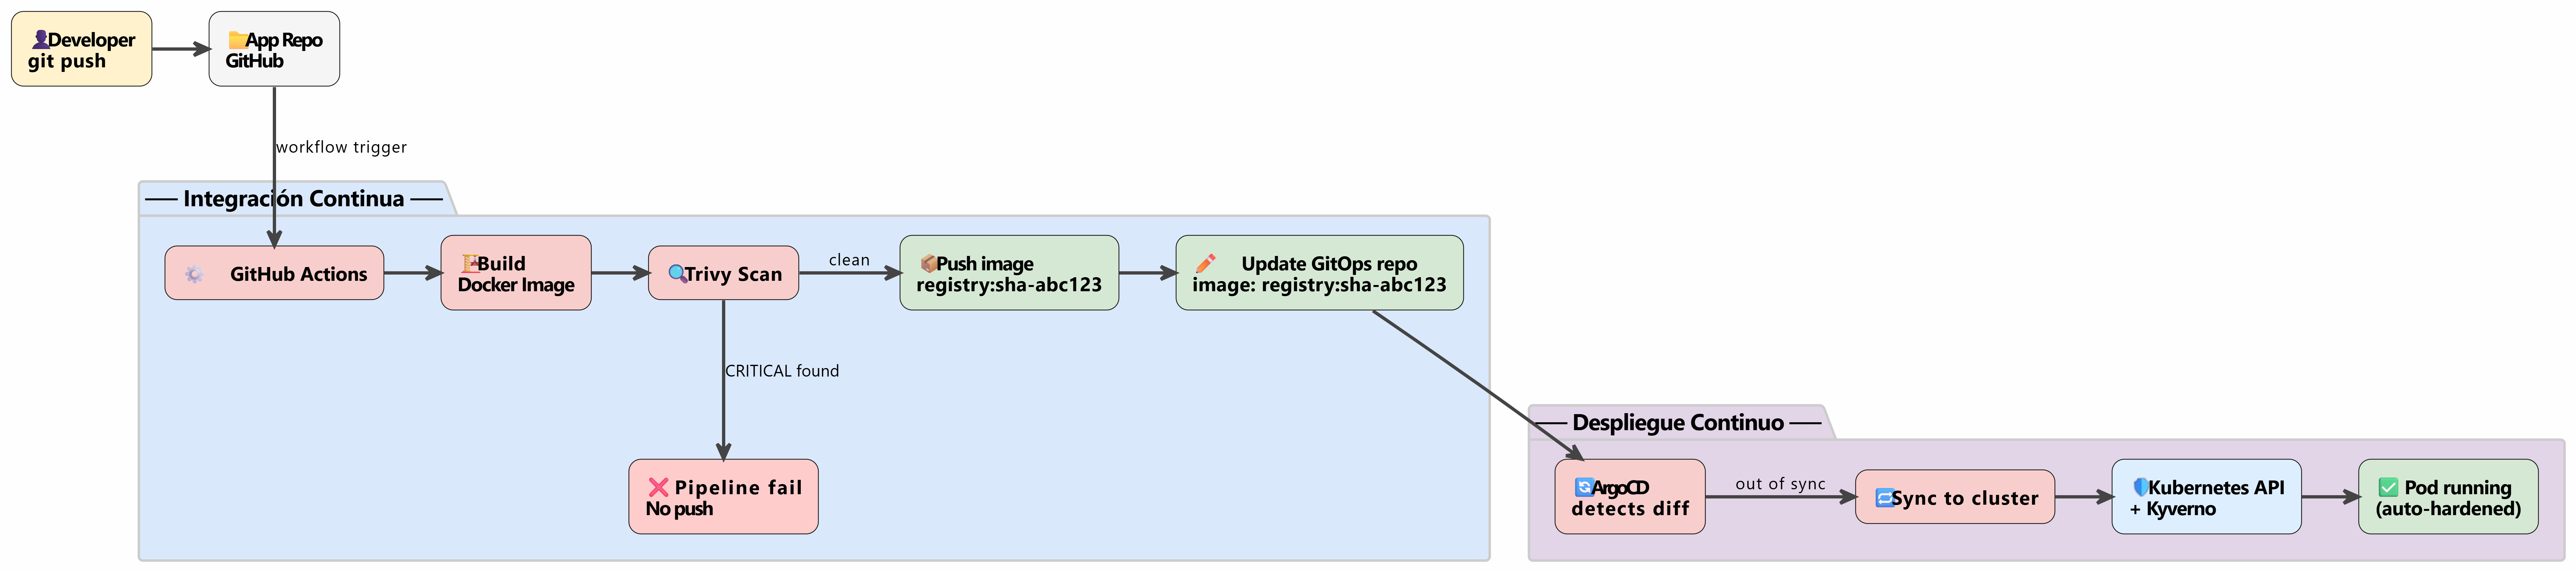
\includegraphics[width=0.95\linewidth]{arquitectura/fig5-2-flujo-cicd.png}
\caption{Flujo de integración y despliegue continuo con análisis de seguridad}
\label{fig:flujo-cicd}
\end{figure}

\subsection{Fase de despliegue continuo y admisión}

ArgoCD monitoriza el repositorio de configuración de forma periódica. Al detectar el nuevo commit introducido por el pipeline de CI, computa la diferencia entre el manifiesto actualizado y el estado actual del clúster e inicia la sincronización, enviando la solicitud de actualización del recurso al API Server de Kubernetes.

En este punto interviene Kyverno a través del mecanismo de Admission Controllers. El proceso de admisión de Kubernetes sigue una secuencia determinada \cite{kubernetes_docs} que se ilustra en la Figura~\ref{fig:flujo-admision}:

\begin{figure}[htbp]
\centering
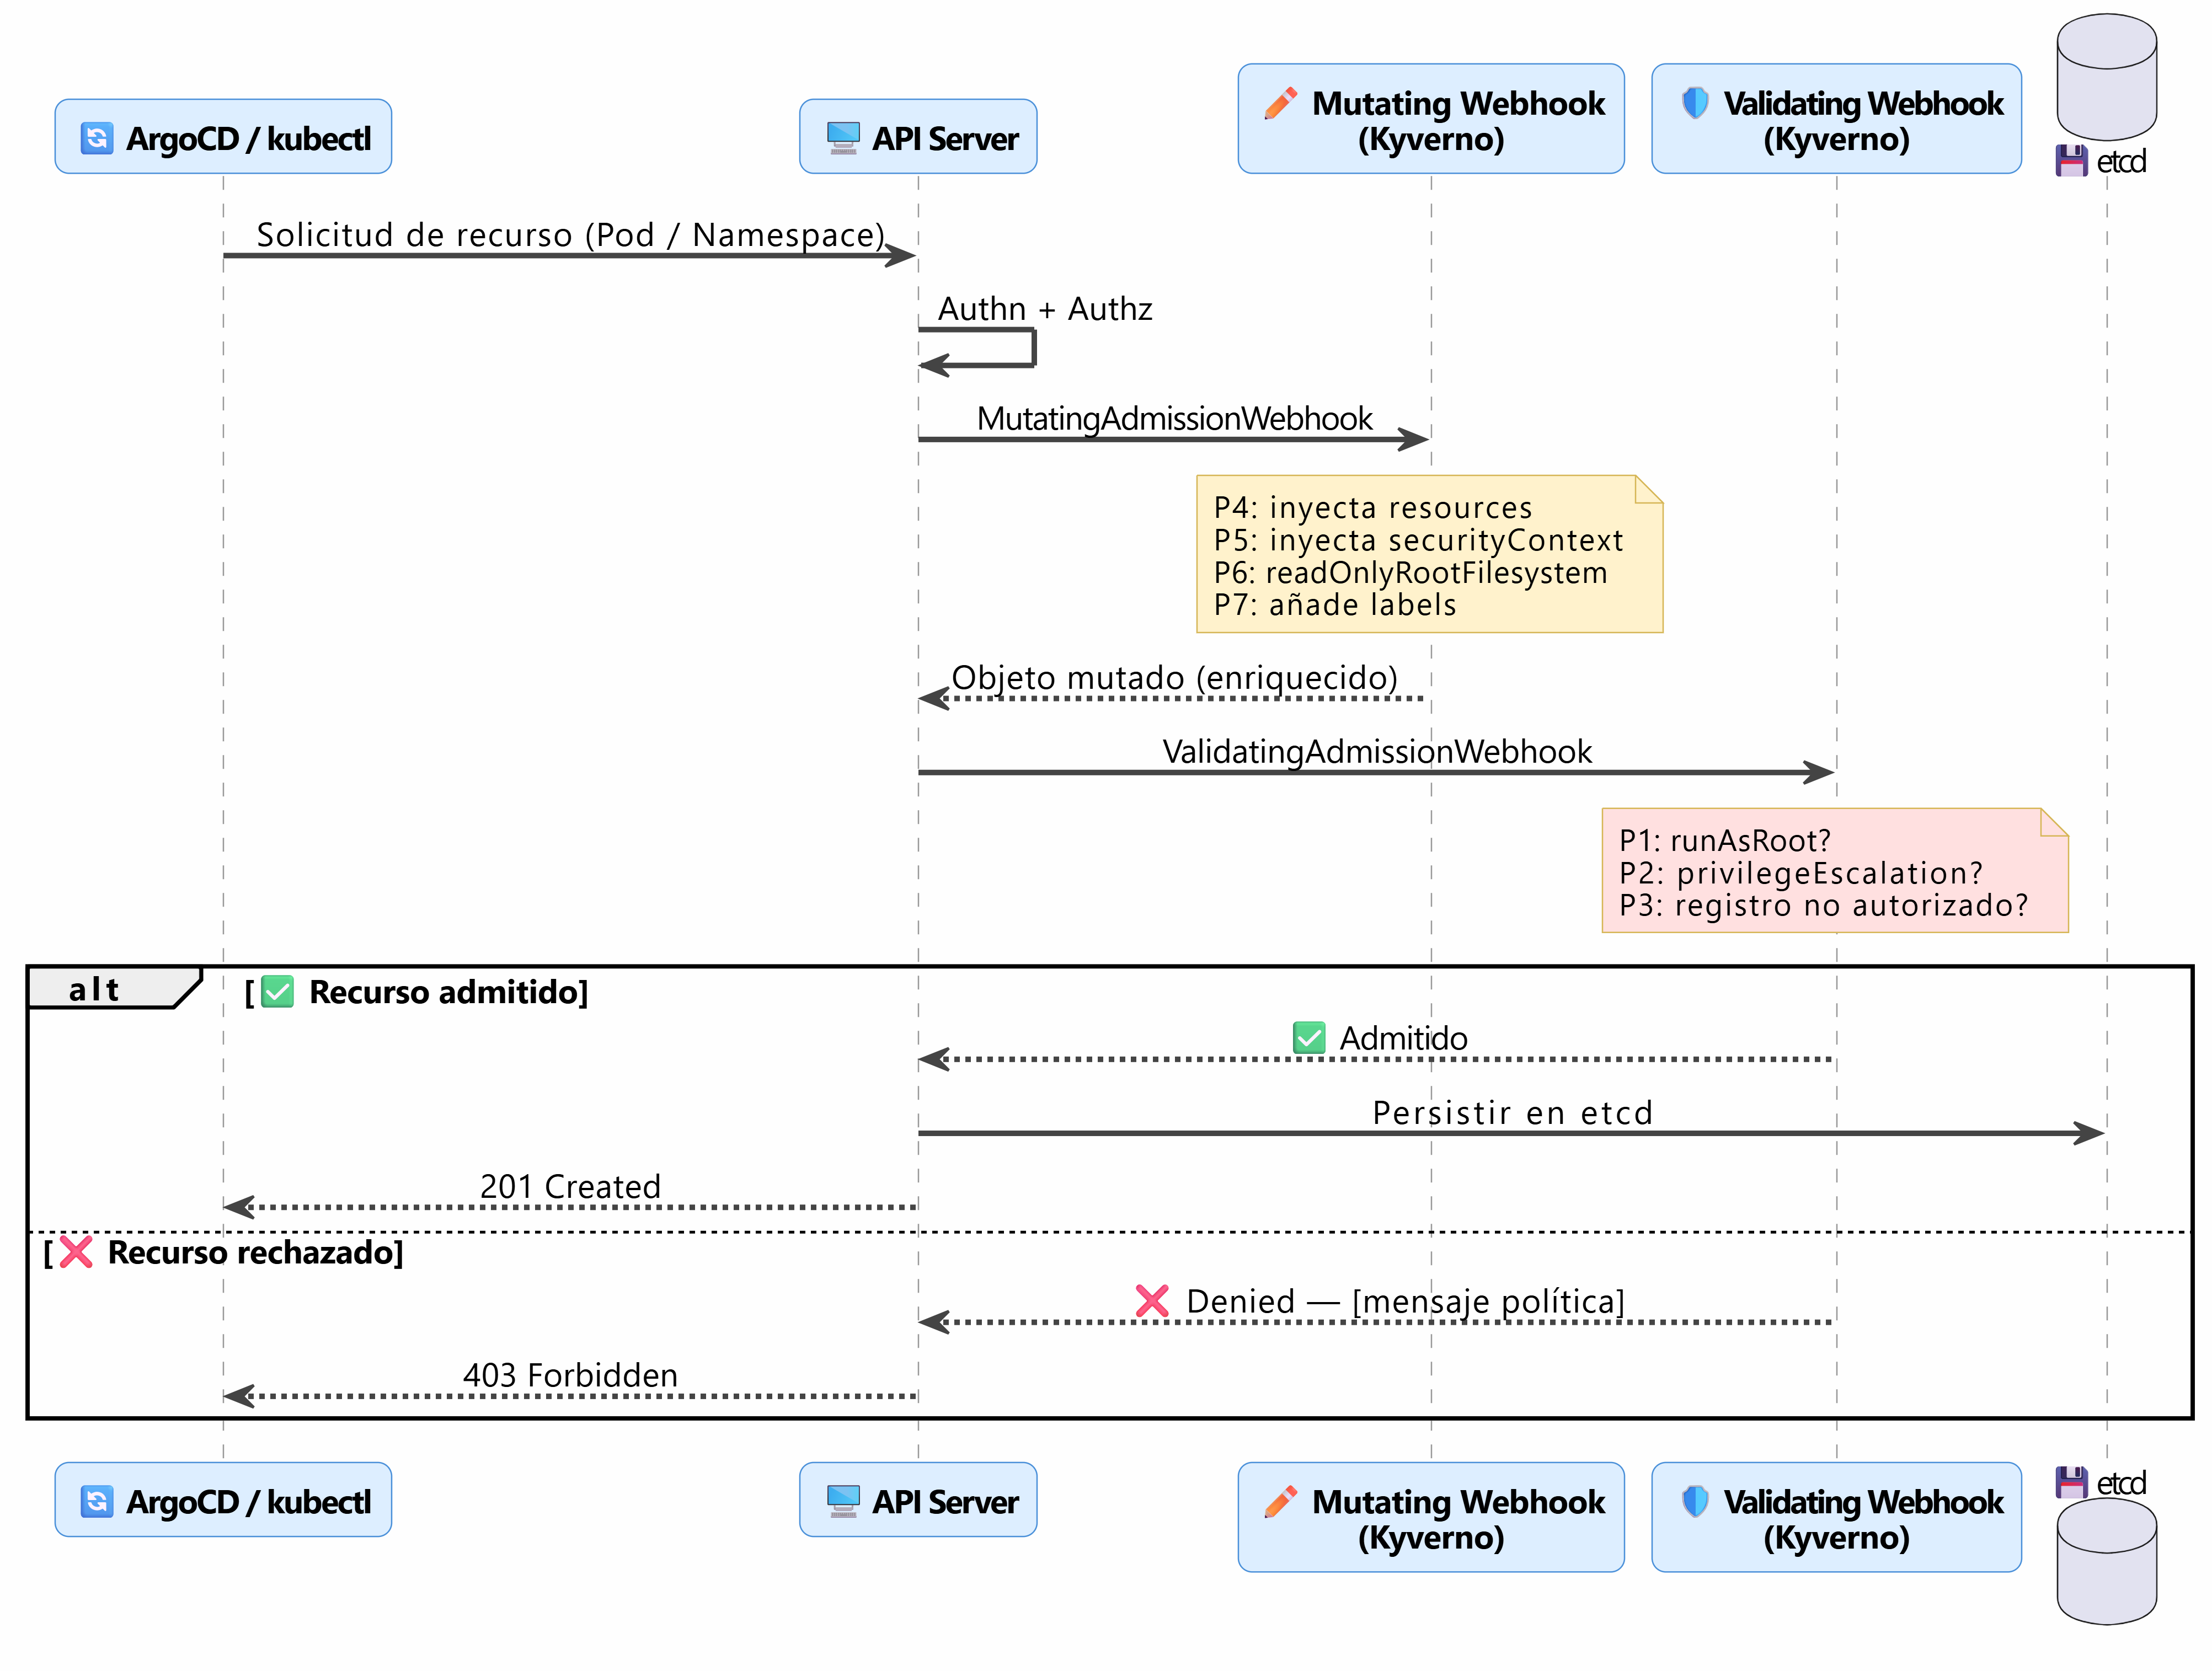
\includegraphics[width=0.90\linewidth]{arquitectura/fig5-3-flujo-admision.png}
\caption{Flujo de admisión de Kyverno: mutación antes de validación}
\label{fig:flujo-admision}
\end{figure}

Tras la autenticación y autorización de la solicitud, el API Server invoca los \textit{mutating admission webhooks} registrados. Kyverno recibe el objeto en su estado original y aplica secuencialmente todas las políticas de tipo \textit{mutate} activas: inyecta los límites y solicitudes de recursos (P4), completa el \texttt{securityContext} del contenedor con las configuraciones seguras faltantes (P5), fuerza el sistema de ficheros de solo lectura (P6) y añade las etiquetas de trazabilidad (P7). El objeto devuelto al API Server es ya la versión enriquecida con todas las configuraciones de seguridad.

A continuación, el API Server invoca los \textit{validating admission webhooks}. Kyverno evalúa las políticas de tipo \textit{validate} sobre el objeto ya mutado. Dado que la mutación ha aplicado previamente las configuraciones seguras, la gran mayoría de pods pasan esta validación sin rechazo. Las políticas de validación actúan como última barrera para casos que la mutación no puede resolver: el uso de imágenes de registros no autorizados (P3), la ejecución explícita como usuario root cuando el desarrollador lo ha especificado de forma deliberada (P1) o la solicitud explícita de escalada de privilegios (P2). Si alguna política de validación rechaza el objeto, el API Server devuelve un error con el mensaje definido en la política y el recurso no es persistido en etcd.

Si el objeto supera todos los webhooks de admisión, es persistido en etcd, el Scheduler determina en qué nodo debe ejecutarse y el kubelet del nodo worker procede con la creación del pod.

\section{Arquitectura de red del clúster}

La topología de red del entorno de laboratorio se articula en tres capas, tal como muestra la Figura~\ref{fig:red-cluster}.

\begin{figure}[htbp]
\centering
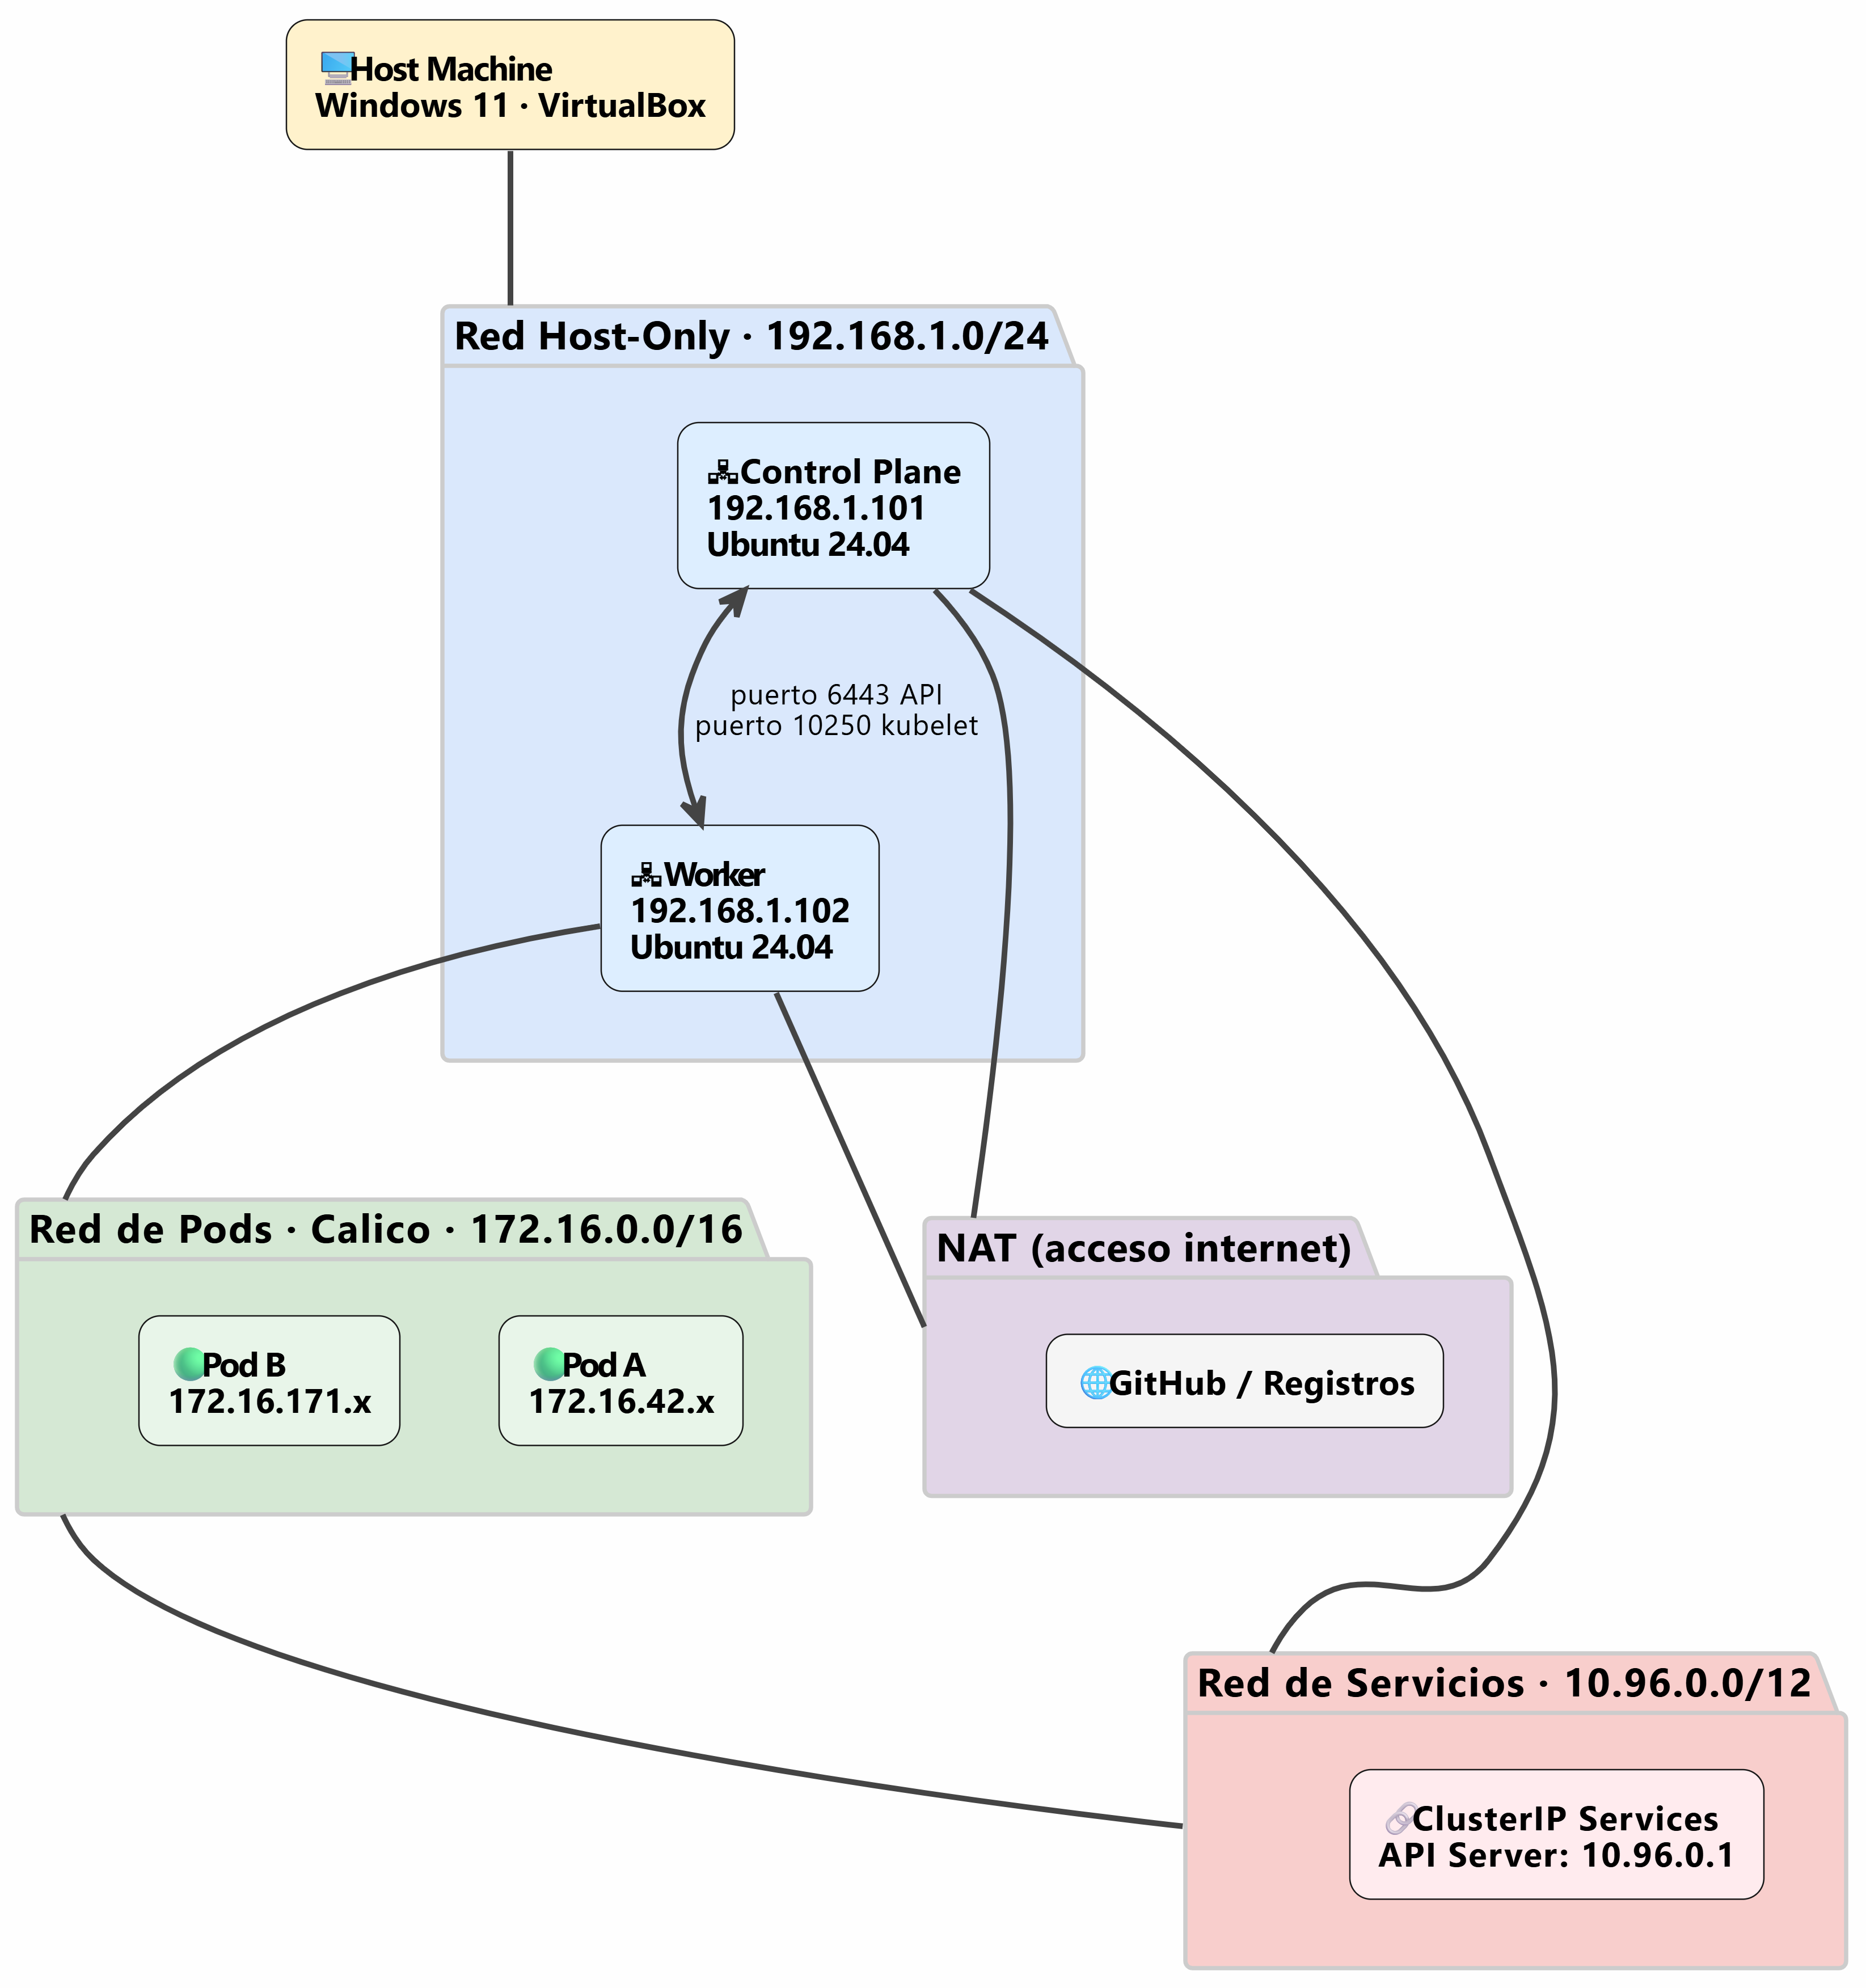
\includegraphics[width=0.85\linewidth]{arquitectura/fig5-4-red-cluster.png}
\caption{Arquitectura de red del clúster de laboratorio}
\label{fig:red-cluster}
\end{figure}

La \textbf{capa de gestión} corresponde a la red \textit{host-only} de VirtualBox (\texttt{192.168.1.0/24}), mediante la cual la máquina anfitriona y ambos nodos del clúster se comunican. Los nodos tienen direcciones IP estáticas asignadas: \texttt{192.168.1.101} para el nodo de control y \texttt{192.168.1.102} para el nodo worker. Toda comunicación interna del clúster —entre el API Server y los kubelets, entre el API Server y los controladores de Kyverno y ArgoCD— transita por esta red. Adicionalmente, cada nodo dispone de una interfaz NAT de VirtualBox que proporciona acceso a internet, utilizada para la descarga de imágenes de contenedor y la comunicación con servicios externos como GitHub o registros de imágenes.

La \textbf{capa de pods} está gestionada por Calico \cite{calico_docs}, que asigna un espacio de direccionamiento privado (\texttt{172.16.0.0/16}) a los pods del clúster. Calico implementa las Network Policies de Kubernetes mediante reglas de \texttt{iptables} o eBPF, en función de la configuración, garantizando que las restricciones de tráfico definidas en las políticas se aplican de forma efectiva. Esta implementación es un requisito para la política P8 del trabajo: la NetworkPolicy generada por Kyverno para bloquear el acceso al servicio de metadatos cloud (\texttt{169.254.169.254/32}) solo tiene efecto si el plugin CNI subyacente respeta y aplica las Network Policies de Kubernetes, condición que Calico cumple de forma nativa.

La \textbf{capa de servicios} utiliza el espacio de direccionamiento \texttt{10.96.0.0/12}, reservado por kubeadm para los objetos \texttt{Service} de tipo \texttt{ClusterIP}. Los servicios de los componentes del sistema —API Server (\texttt{10.96.0.1}), ArgoCD Server, Kyverno— son accesibles dentro del clúster a través de este espacio de direcciones, mientras que el acceso externo al API Server se realiza directamente a través de la IP del nodo de control mediante el puerto 6443.

% ─────────────────────────────────────────────
\section{Decisiones de diseño}
\label{sec:decisiones}
% ─────────────────────────────────────────────

Las decisiones arquitectónicas adoptadas en el diseño del sistema no son arbitrarias, sino que responden a requisitos técnicos y de seguridad concretos. Esta sección documenta las más relevantes y justifica cada una de ellas.

\subsection{Separación entre CI y CD}

La separación entre integración continua (GitHub Actions) y despliegue continuo (ArgoCD) es una decisión arquitectónica deliberada, en lugar de un único pipeline que construye y despliega en una sola secuencia. Esta separación ofrece varias ventajas. En primer lugar, desacopla las credenciales necesarias: el pipeline de CI necesita acceso al registro de imágenes y al repositorio de configuración, pero no al clúster Kubernetes; ArgoCD tiene acceso al clúster pero no al código fuente. Esta segregación reduce el radio de impacto de un posible compromiso de cualquiera de los dos componentes. En segundo lugar, permite aplicar controles de seguridad en el límite entre ambas fases: la imagen solo es publicada si pasa el análisis de Trivy, y ArgoCD solo despliega lo que está en el repositorio de configuración, que actúa como punto de control auditado.

\subsection{Alcance de ClusterPolicy frente a Policy}

Kyverno permite definir políticas con alcance de clúster (\texttt{ClusterPolicy}) o con alcance de namespace (\texttt{Policy}). En este trabajo se utilizan exclusivamente \texttt{ClusterPolicy}, lo que garantiza que las políticas de seguridad se aplican a todos los namespaces del clúster sin excepciones. Una política namespaced podría ser inadvertidamente omitida al crear un nuevo namespace, creando una brecha de cobertura. El uso de \texttt{ClusterPolicy} implementa el principio de \textit{secure by default}: la seguridad se aplica en todas partes a menos que sea explícitamente excluida mediante reglas de excepción documentadas.

\subsection{Modo Enforce frente a Audit}

Kyverno permite operar en dos modos: \texttt{Enforce}, que bloquea activamente los recursos que incumplen las políticas, y \texttt{Audit}, que permite el despliegue pero registra las infracciones en los PolicyReports. En este trabajo, las políticas de validación operan en modo \texttt{Enforce}, lo que garantiza que ningún recurso no conforme llega al clúster. Aunque en un entorno de producción real suele recomendarse comenzar en modo \texttt{Audit} para evitar interrupciones, en el contexto de este entorno de laboratorio el modo \texttt{Enforce} es el que permite demostrar de forma efectiva el mecanismo de bloqueo y su efecto real sobre los despliegues.

\subsection{Mutación antes de validación como estrategia de hardening}

El orden de ejecución de los webhooks de Kubernetes —mutación antes de validación— se aprovecha deliberadamente como estrategia de \textit{hardening} automático. Las políticas de mutación no son complementos opcionales, sino el mecanismo principal de seguridad del sistema: en lugar de rechazar pods con configuraciones incompletas (lo que generaría fricción para los desarrolladores), Kyverno los completa automáticamente con el perfil de seguridad correcto. Las políticas de validación actúan únicamente sobre las configuraciones que no pueden resolverse mediante mutación, como el uso de registros de imágenes no autorizados o la presencia de privilegios explícitamente declarados.

Esta estrategia alinea seguridad y usabilidad: el desarrollador puede trabajar con manifiestos mínimos y obtener un pod correctamente securizado sin necesidad de conocer en detalle todos los campos de seguridad de Kubernetes. La responsabilidad del cumplimiento recae en la plataforma, no en el desarrollador.

\subsection{synchronize: true en políticas de generación}

La política P8 utiliza el campo \texttt{synchronize: true} en su definición de tipo \textit{generate}. Esta configuración instruye al Background Controller de Kyverno para que monitorice los recursos generados y los recree automáticamente si son eliminados o modificados de forma no autorizada. Esta decisión implementa el principio de \textit{drift protection} a nivel de recursos de seguridad: la NetworkPolicy que bloquea el acceso al IMDS no puede ser eliminada de forma permanente por un operador (intencionada o accidentalmente), ya que Kyverno la regenerará en cuestión de segundos. Sin este campo, la generación sería un evento único y la protección podría ser eludida.

\subsection{Seguridad de la cadena de suministro del pipeline}

El compromiso del grupo TeamPCP sobre pipelines CI/CD \cite{teampcp2026} ilustra que el propio pipeline de automatización puede convertirse en vector de ataque. En respuesta a esta amenaza, el diseño del pipeline adopta dos medidas concretas. La primera es el anclaje de versiones de las GitHub Actions utilizadas mediante su hash SHA completo, en lugar de etiquetas flotantes como \texttt{@latest} o \texttt{@v3}, que pueden ser redirigidas a versiones maliciosas sin modificar el nombre de la referencia. La segunda es la configuración del token de GitHub con permisos mínimos (\textit{least privilege}): el runner solo dispone de los permisos estrictamente necesarios para su función, limitando el impacto de un posible compromiso del entorno de ejecución.

\subsection{Elección de Calico como plugin CNI}

La elección de Calico \cite{calico_docs} frente a alternativas como Flannel o Weave responde a un requisito funcional directo: la política P8 requiere que las Network Policies de Kubernetes sean aplicadas efectivamente por el plugin CNI. Flannel, por ejemplo, no implementa soporte para Network Policies de forma nativa. Calico, en cambio, es uno de los plugins CNI de referencia en entornos de producción y proporciona una implementación completa del modelo de Network Policy de Kubernetes, garantizando que las reglas de bloqueo de tráfico generadas por Kyverno tienen efecto real sobre la comunicación de red de los pods.

% ─────────────────────────────────────────────
% DIAGRAMAS MERMAID — EXPORTAR A PNG Y GUARDAR EN images/arquitectura/
% ─────────────────────────────────────────────
%
% FIGURA 5.1 — Arquitectura general (guardar como: images/arquitectura/fig5-1-arquitectura-general.png)
%
% flowchart TB
%     subgraph PLANO_DEV["Plano de Desarrollo"]
%         direction LR
%         DEV["👤 Desarrollador"]
%         APP_REPO["📁 Repositorio\nde Aplicación\n(GitHub)"]
%         CFG_REPO["📁 Repositorio\nde Configuración\n(GitOps repo)"]
%     end
%
%     subgraph PLANO_AUTO["Plano de Automatización"]
%         direction LR
%         GA["⚙️ GitHub Actions\n(CI Pipeline)"]
%         TRIVY["🔍 Trivy\nVulnerability Scanner"]
%         REGISTRY["📦 Registro\nde Imágenes"]
%         ARGO["🔄 ArgoCD\n(CD GitOps)"]
%     end
%
%     subgraph PLANO_EXEC["Plano de Ejecución — Clúster Kubernetes"]
%         subgraph CP["Control Plane · 192.168.1.101"]
%             API["API Server"]
%             ETCD[("etcd")]
%             KYVERNO["🛡️ Kyverno\nAdmission Controller"]
%         end
%         subgraph WK["Worker · 192.168.1.102"]
%             PODS["🟢 Pods\n(securizados)"]
%         end
%     end
%
%     DEV -->|"git push"| APP_REPO
%     DEV -->|"git push policies"| CFG_REPO
%     APP_REPO -->|"trigger"| GA
%     GA --> TRIVY
%     TRIVY -->|"imagen limpia"| REGISTRY
%     GA -->|"actualiza imagen tag"| CFG_REPO
%     CFG_REPO -->|"detecta cambios"| ARGO
%     ARGO -->|"kubectl apply"| API
%     API --> KYVERNO
%     KYVERNO -->|"objeto mutado\n+ validado"| ETCD
%     ETCD --> PODS
%
%
% FIGURA 5.2 — Flujo CI/CD (guardar como: images/arquitectura/fig5-2-flujo-cicd.png)
%
% flowchart LR
%     DEV["👤 Developer\ngit push"] --> APP_REPO["App Repo\nGitHub"]
%     APP_REPO -->|"workflow trigger"| GA["GitHub Actions"]
%
%     subgraph CI["── Integración Continua ──"]
%         GA --> BUILD["Build\nDocker Image"]
%         BUILD --> SCAN["Trivy Scan"]
%         SCAN -->|"CRITICAL found"| FAIL["❌ Pipeline fail\nNo push"]
%         SCAN -->|"clean"| PUSH["Push image\nregistry:sha-abc123"]
%         PUSH --> UPDATE["Update GitOps repo\nimage: registry:sha-abc123"]
%     end
%
%     subgraph CD["── Despliegue Continuo ──"]
%         UPDATE --> ARGO["ArgoCD\ndetects diff"]
%         ARGO -->|"out of sync"| SYNC["Sync to cluster"]
%         SYNC --> K8S["Kubernetes API\n+ Kyverno"]
%         K8S --> POD["✅ Pod running\n(auto-hardened)"]
%     end
%
%
% FIGURA 5.3 — Flujo de admisión Kyverno (guardar como: images/arquitectura/fig5-3-flujo-admision.png)
%
% sequenceDiagram
%     participant C as ArgoCD / kubectl
%     participant A as API Server
%     participant M as Mutating Webhook\n(Kyverno)
%     participant V as Validating Webhook\n(Kyverno)
%     participant E as etcd
%
%     C->>A: Solicitud de recurso (Pod / Namespace)
%     A->>A: Authn + Authz
%     A->>M: MutatingAdmissionWebhook
%     note over M: P4: inyecta resources\nP5: inyecta securityContext\nP6: readOnlyRootFilesystem\nP7: añade labels
%     M-->>A: Objeto mutado (enriquecido)
%     A->>V: ValidatingAdmissionWebhook
%     note over V: P1: runAsRoot?\nP2: privilegeEscalation?\nP3: registro no autorizado?
%     alt Recurso admitido
%         V-->>A: ✅ Admitido
%         A->>E: Persistir en etcd
%         A-->>C: 201 Created
%     else Recurso rechazado
%         V-->>A: ❌ Denied — [mensaje política]
%         A-->>C: 403 Forbidden
%     end
%
%
% FIGURA 5.4 — Arquitectura de red (guardar como: images/arquitectura/fig5-4-red-cluster.png)
%
% flowchart TB
%     HOST["🖥️ Host Machine\nWindows 11 · VirtualBox"]
%
%     subgraph HOSTONLYNET["Red Host-Only · 192.168.1.0/24"]
%         CP["Control Plane\n192.168.1.101\nUbuntu 24.04"]
%         WK["Worker\n192.168.1.102\nUbuntu 24.04"]
%     end
%
%     subgraph NATNET["NAT (acceso internet)"]
%         GH["GitHub / Registros"]
%     end
%
%     subgraph PODNET["Red de Pods · Calico\n172.16.0.0/16"]
%         P1["Pod A · 10.244.1.x"]
%         P2["Pod B · 10.244.2.x"]
%     end
%
%     subgraph SVCNET["Red de Servicios\n10.96.0.0/12"]
%         SVC["ClusterIP Services\nAPI Server: 10.96.0.1"]
%     end
%
%     HOST --- HOSTONLYNET
%     CP <-->|"puerto 6443 API\npuerto 10250 kubelet"| WK
%     CP --- NATNET
%     WK --- NATNET
%     WK --- PODNET
%     PODNET --- SVCNET
%     CP --- SVCNET

\chapter{Implementación}

El presente capítulo documenta la implementación práctica del entorno DevSecOps descrito en los capítulos anteriores. A diferencia del Capítulo~5, que establece el diseño y las decisiones arquitectónicas, este capítulo se centra en la ejecución concreta: los pasos realizados, las políticas desplegadas con sus manifiestos completos, las pruebas ejecutadas y los resultados observados. Cada sección incluye evidencia directa del sistema en funcionamiento mediante capturas del entorno real.

% ─────────────────────────────────────────────
\section{Aprovisionamiento del clúster Kubernetes}
% ─────────────────────────────────────────────

El punto de partida del proyecto es el aprovisionamiento de un clúster Kubernetes funcional sobre el entorno de laboratorio descrito en la Sección~4.2. Las máquinas virtuales, proporcionadas por el tutor, ejecutan Ubuntu Server 24.04 LTS y están preconfiguradas con los paquetes necesarios (\texttt{kubeadm}, \texttt{kubelet}, \texttt{kubectl}) y con la capa de red de VirtualBox en modo NAT más \textit{host-only adapter}.

La inicialización del plano de control se realiza desde el nodo \texttt{control} (\texttt{192.168.1.101}) mediante el comando:

\begin{center}
\begin{minipage}{0.88\linewidth}
\begin{verbatim}
sudo kubeadm init --apiserver-advertise-address=192.168.1.101
\end{verbatim}
\end{minipage}
\end{center}

El parámetro \texttt{--apiserver-advertise-address} es necesario en entornos con múltiples interfaces de red para indicar a kubeadm en qué dirección debe escuchar el API Server. Sin este parámetro, kubeadm seleccionaría la interfaz por defecto, que en VirtualBox corresponde al adaptador NAT (\texttt{10.0.2.x}), inaccesible desde el nodo worker. Especificando la dirección de la interfaz \textit{host-only}, se garantiza que los componentes del clúster —incluidos los webhooks de Kyverno— son alcanzables a través de la red interna del laboratorio.

Tras la inicialización, se configura el acceso a \texttt{kubectl} para el usuario \texttt{student} copiando el fichero de configuración generado por kubeadm:

\begin{center}
\begin{minipage}{0.88\linewidth}
\begin{verbatim}
mkdir -p $HOME/.kube
sudo cp -i /etc/kubernetes/admin.conf $HOME/.kube/config
sudo chown $(id -u):$(id -g) $HOME/.kube/config
\end{verbatim}
\end{minipage}
\end{center}

A continuación, el nodo worker (\texttt{192.168.1.102}) se incorpora al clúster mediante el comando \texttt{kubeadm join} generado durante la inicialización, que incluye el token de arranque y el hash del certificado del API Server para garantizar la autenticidad de la conexión.

Una vez que ambos nodos forman parte del clúster, se instala el plugin CNI Calico en su versión 3.28:

\begin{center}
\begin{minipage}{0.88\linewidth}
\begin{verbatim}
kubectl apply -f https://raw.githubusercontent.com/projectcalico/
calico/v3.28.0/manifests/calico.yaml
\end{verbatim}
\end{minipage}
\end{center}

Calico configura el espacio de direccionamiento de pods con el CIDR \texttt{172.16.0.0/16}, que es el valor por defecto asignado por esta distribución de Calico. Una vez completada la instalación y tras la convergencia de los componentes del sistema, el clúster alcanza el estado operativo con ambos nodos en estado \texttt{Ready}.

% ─────────────────────────────────────────────
\section{Despliegue e integración de Kyverno}
% ─────────────────────────────────────────────

Con el clúster operativo, el siguiente paso es la instalación de Kyverno como motor de políticas de seguridad. Kyverno se despliega mediante Helm en el namespace dedicado \texttt{kyverno}, con todos sus controladores en modo \textit{standalone}:

\begin{center}
\begin{minipage}{0.88\linewidth}
\begin{verbatim}
helm repo add kyverno https://kyverno.github.io/kyverno/
helm repo update
helm install kyverno kyverno/kyverno -n kyverno --create-namespace
\end{verbatim}
\end{minipage}
\end{center}

Tras la instalación, la verificación del estado de los pods en el namespace \texttt{kyverno} confirma que los cuatro controladores están activos y en estado \texttt{Running}, como muestra la Figura~\ref{fig:kyverno-pods}.

\begin{figure}[H]
\centering
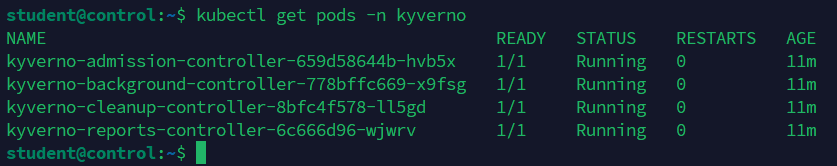
\includegraphics[width=0.85\linewidth]{kyverno/compKyverno.png}
\caption{Controladores de Kyverno desplegados en el clúster}
\label{fig:kyverno-pods}
\end{figure}

Los cuatro controladores —\texttt{admission-controller}, \texttt{background-controller}, \texttt{cleanup-controller} y \texttt{reports-controller}— operan de forma independiente y complementaria, tal como se describió en la Sección~5.2.2. El controlador más relevante para el comportamiento en tiempo real del sistema es el \textit{admission controller}, que se registra en el API Server inmediatamente tras su despliegue.

La verificación de los webhooks registrados confirma que Kyverno ha establecido correctamente su integración con el API Server. La consulta de los objetos \texttt{ValidatingWebhookConfiguration} muestra siete configuraciones registradas por Kyverno, como se aprecia en la Figura~\ref{fig:kyverno-webhooks}.

\begin{figure}[H]
\centering
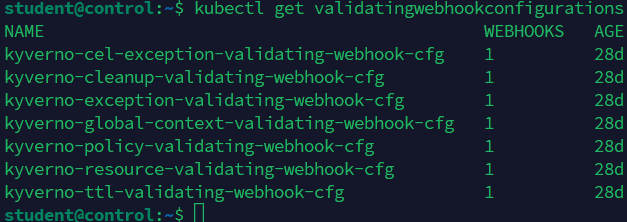
\includegraphics[width=0.85\linewidth]{kyverno/webhooksKyverno.png}
\caption{ValidatingWebhookConfiguration registradas por Kyverno en el API Server}
\label{fig:kyverno-webhooks}
\end{figure}

Entre las configuraciones registradas, la más relevante para este trabajo es \texttt{kyverno-resource-validating-webhook-cfg}, que intercepta las solicitudes de creación y modificación de recursos arbitrarios del clúster y las deriva al \textit{admission controller} de Kyverno para su evaluación. Las configuraciones adicionales cubren casos específicos como la validación de las propias políticas (\texttt{kyverno-policy-validating-webhook-cfg}), el contexto global (\texttt{kyverno-global-context-validating-webhook-cfg}) y la gestión de excepciones y TTL. Análogamente, Kyverno registra las correspondientes configuraciones \texttt{MutatingWebhookConfiguration} para el procesamiento de las políticas de tipo \textit{mutate}.

Con Kyverno instalado y sus webhooks activos, el clúster está listo para recibir políticas de seguridad. La Figura~\ref{fig:estado-inicial} muestra el estado del clúster en este punto, antes de aplicar ninguna política: la consulta de \texttt{ClusterPolicy} no devuelve ningún recurso.

\begin{figure}[H]
\centering
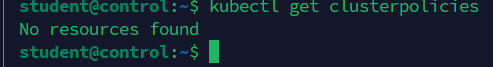
\includegraphics[width=0.55\linewidth]{kyverno/estadoInicial.png}
\caption{Estado inicial del clúster: sin políticas desplegadas}
\label{fig:estado-inicial}
\end{figure}

% ─────────────────────────────────────────────
\section{Políticas de validación}
% ─────────────────────────────────────────────

Las políticas de validación constituyen la capa reactiva del sistema de seguridad: actúan rechazando recursos que incumplen condiciones que no pueden resolverse mediante mutación automática. Como se justificó en la Sección~5.5.4, las políticas de mutación tienen precedencia y actúan antes, por lo que las de validación operan como barrera final para configuraciones explícitamente inseguras que no deben corregirse de forma silenciosa, sino rechazarse con un mensaje claro.

\subsection{Política P1: \texttt{disallow-root}}

La primera política de validación impide el despliegue de pods que no especifiquen explícitamente que sus contenedores deben ejecutarse como un usuario no root. El manifiesto completo es el siguiente:

\begin{center}
\begin{minipage}{0.88\linewidth}
\begin{verbatim}
apiVersion: kyverno.io/v1
kind: ClusterPolicy
metadata:
  name: disallow-root
spec:
  validationFailureAction: Enforce
  background: true
  rules:
  - name: require-run-as-non-root
    match:
      any:
      - resources:
          kinds:
          - Pod
    validate:
      message: "Containers must not run as root"
      pattern:
        spec:
          securityContext:
            runAsNonRoot: true
\end{verbatim}
\end{minipage}
\end{center}

La política opera mediante un mecanismo de \textit{pattern matching}: Kyverno verifica que el campo \texttt{spec.securityContext.runAsNonRoot} existe y tiene el valor \texttt{true}. Si el campo está ausente o es \texttt{false}, el webhook devuelve un error de validación con el mensaje definido y la solicitud es rechazada.

La justificación técnica de este control es doble. En primer lugar, un proceso que ejecuta como \texttt{UID 0} dentro del contenedor hereda el conjunto completo de capacidades del kernel de Linux asignado al contenedor, incluyendo \texttt{CAP\_SYS\_ADMIN}, \texttt{CAP\_NET_RAW} y otras que amplían significativamente la superficie de ataque. En segundo lugar, si se produce un escape del aislamiento del contenedor —ya sea mediante una vulnerabilidad del runtime o del kernel—, un proceso que ya ejecutaba como root en el contenedor obtendrá privilegios de root en el nodo anfitrión, comprometiendo la totalidad del nodo y potencialmente el clúster.

La prueba de validación se realiza aplicando el siguiente pod, que no especifica ningún \texttt{securityContext}:

\begin{center}
\begin{minipage}{0.88\linewidth}
\begin{verbatim}
apiVersion: v1
kind: Pod
metadata:
  name: nginx-inseguro
spec:
  containers:
  - name: nginx
    image: nginx
\end{verbatim}
\end{minipage}
\end{center}

El resultado, mostrado en la Figura~\ref{fig:test1}, confirma que el webhook de Kyverno rechaza la solicitud con el mensaje de error de la política, indicando el path exacto del campo que falla (\texttt{/spec/securityContext/runAsNonRoot/}).

\begin{figure}[H]
\centering
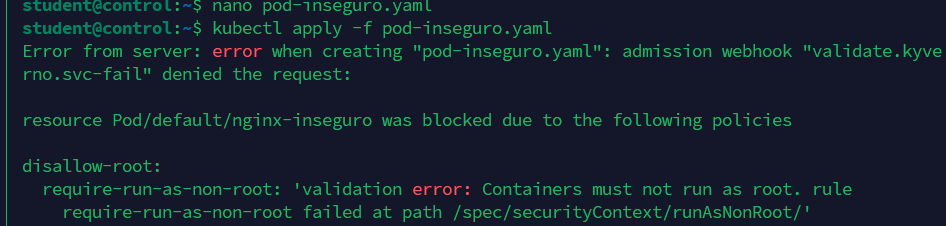
\includegraphics[width=0.95\linewidth]{kyverno/test1.png}
\caption{P1: bloqueo de pod sin \texttt{runAsNonRoot} por el webhook de Kyverno}
\label{fig:test1}
\end{figure}

\subsection{Política P2: \texttt{disallow-privilege-escalation}}

La segunda política de validación exige que todos los contenedores declaren explícitamente \texttt{allowPrivilegeEscalation: false} en su \texttt{securityContext} a nivel de contenedor:

\begin{center}
\begin{minipage}{0.88\linewidth}
\begin{verbatim}
apiVersion: kyverno.io/v1
kind: ClusterPolicy
metadata:
  name: disallow-privilege-escalation
spec:
  validationFailureAction: Enforce
  rules:
  - name: no-privilege-escalation
    match:
      any:
      - resources:
          kinds:
          - Pod
    validate:
      message: "Privilege escalation is not allowed"
      pattern:
        spec:
          containers:
          - securityContext:
              allowPrivilegeEscalation: false
\end{verbatim}
\end{minipage}
\end{center}

Este campo controla el flag \texttt{no\_new\_privs} del kernel Linux, introducido en la versión 3.5. Cuando está activo, impide que cualquier proceso hijo del contenedor adquiera más privilegios que su proceso padre, bloqueando de forma efectiva los ataques basados en la ejecución de binarios con el bit \texttt{SUID} o \texttt{SGID} activo. Sin este flag, un proceso que ejecuta con \texttt{UID} no privilegiado podría invocar un binario como \texttt{sudo} o \texttt{su} con bit SUID para elevar sus privilegios al de root, eludiendo los controles de \texttt{runAsNonRoot}.

La prueba aplica un pod que solicita escalada de privilegios de forma explícita. El resultado, capturado en la Figura~\ref{fig:test2}, muestra el rechazo por el webhook con el path del campo infractor (\texttt{/spec/containers/0/securityContext/allowPrivilegeEscalation/}).

\begin{figure}[H]
\centering
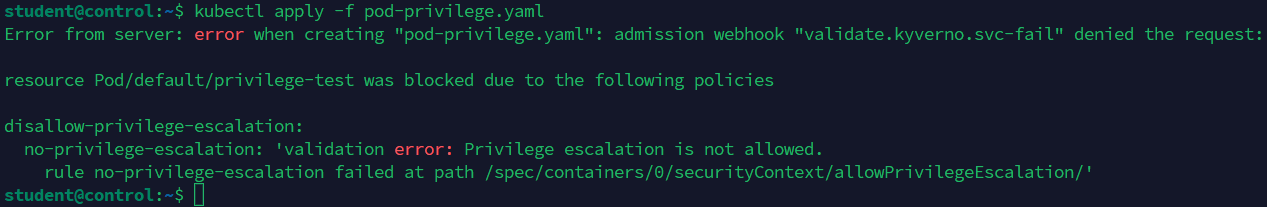
\includegraphics[width=0.95\linewidth]{kyverno/test2.png}
\caption{P2: bloqueo de pod con \texttt{allowPrivilegeEscalation: true}}
\label{fig:test2}
\end{figure}

Es importante destacar la interacción entre esta política y la política de mutación P5, descrita en la Sección~6.4.2. Dado que el flujo de admisión de Kubernetes invoca los \textit{mutating webhooks} antes que los \textit{validating webhooks}, la política P5 inyecta \texttt{allowPrivilegeEscalation: false} automáticamente en pods que no especifican este campo. En consecuencia, P2 actúa únicamente como barrera final para los casos en que el valor \texttt{true} ha sido declarado de forma explícita en el manifiesto —una declaración de intención insegura que no debe ser corregida silenciosamente, sino rechazada.

\subsection{Política P3: \texttt{restrict-image-registries}}

La tercera política de validación restringe los registros de imágenes de contenedor a un conjunto de fuentes verificadas. Se implementa mediante el mecanismo \texttt{foreach} de Kyverno, que permite evaluar condiciones sobre listas de elementos:

\begin{center}
\begin{minipage}{0.88\linewidth}
\begin{verbatim}
apiVersion: kyverno.io/v1
kind: ClusterPolicy
metadata:
  name: restrict-image-registries
spec:
  validationFailureAction: Enforce
  background: true
  rules:
  - name: validate-registries
    match:
      any:
      - resources:
          kinds:
          - Pod
    validate:
      message: >-
        Solo se permiten imágenes de registros autorizados:
        docker.io, ghcr.io, registry.k8s.io, quay.io.
        La imagen {{ element.image }} no está permitida.
      foreach:
      - list: "request.object.spec.containers"
        deny:
          conditions:
            all:
            - key: "{{ element.image }}"
              operator: AnyNotIn
              value:
              - "docker.io/*"
              - "ghcr.io/*"
              - "registry.k8s.io/*"
              - "quay.io/*"
              - "nginx*"
              - "alpine*"
              - "busybox*"
              - "nginxinc/*"
\end{verbatim}
\end{minipage}
\end{center}

La política itera sobre todos los contenedores del pod y deniega la solicitud si alguna imagen no pertenece a los patrones de registro autorizados. Los patrones sin prefijo de registro (\texttt{nginx*}, \texttt{alpine*}, \texttt{busybox*}) son necesarios porque Kubernetes resuelve implícitamente las referencias de imagen sin prefijo hacia Docker Hub, y las pruebas del proyecto utilizan estas imágenes en su forma abreviada. La inclusión de \texttt{ghcr.io/*} es también un requisito operativo, dado que las propias imágenes de Kyverno y otros componentes del clúster se distribuyen a través de este registro.

Esta política constituye una primera línea de defensa frente a ataques a la cadena de suministro del tipo documentado por el grupo TeamPCP \cite{teampcp2026}: un atacante que consiguiera alojar una imagen maliciosa en un registro arbitrario no podría ejecutarla en el clúster sin modificar esta política. En entornos de producción maduros, este control se complementaría con verificación de firmas digitales mediante Cosign o Notary —una línea de trabajo futuro mencionada en la Sección~4.7.

Durante la implementación de esta política se observó un comportamiento relevante del motor de Kyverno: la variable \texttt{\{\{ element.image \}\}} referenciada en el campo \texttt{message} de nivel superior de la regla no se expande durante la evaluación, dado que dicha variable solo tiene scope dentro del bloque \texttt{foreach}. Kyverno acepta la política como válida —el campo \texttt{READY} aparece como \texttt{True}—, pero en el momento del rechazo el mensaje de error muestra únicamente la parte estática de la cadena, omitiendo la referencia a la imagen específica que causó el bloqueo. Este comportamiento ilustra una característica del modelo de scoping de variables de Kyverno que debe tenerse en cuenta al diseñar mensajes de error informativos en políticas con \texttt{foreach}.

La prueba de validación aplica un pod que referencia una imagen de un registro no autorizado. El resultado, capturado en la Figura~\ref{fig:test3}, revela un comportamiento de defensa en profundidad: el pod es bloqueado simultáneamente por dos políticas independientes.

\begin{figure}[H]
\centering
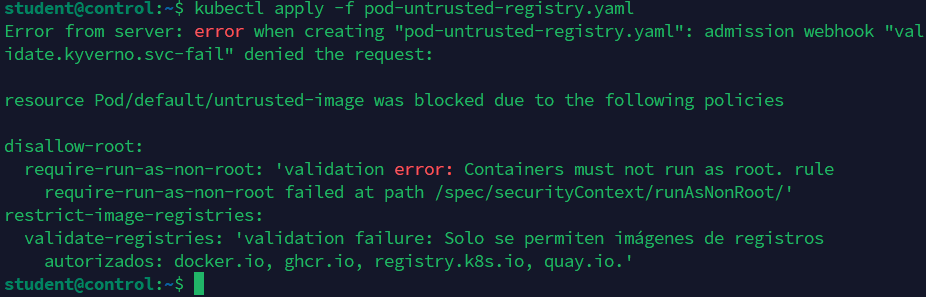
\includegraphics[width=0.95\linewidth]{kyverno/test3.png}
\caption{P3: bloqueo simultáneo por \texttt{disallow-root} y \texttt{restrict-image-registries}}
\label{fig:test3}
\end{figure}

Este resultado evidencia que el sistema de políticas actúa de forma acumulativa: el mismo recurso puede violar múltiples políticas simultáneamente, y el mensaje de error devuelto enumera todas las infracciones detectadas. La imagen \texttt{evilregistry.io/backdoor:latest} es bloqueada tanto por no especificar \texttt{runAsNonRoot} (P1) como por provenir de un registro no autorizado (P3), dos vectores de riesgo independientes que el sistema detecta y reporta en una única respuesta.

% ─────────────────────────────────────────────
\section{Políticas de mutación}
% ─────────────────────────────────────────────

Las políticas de mutación constituyen el mecanismo principal de seguridad del sistema, alineándose con la hipótesis central del trabajo: que la corrección automática de configuraciones inseguras en tiempo de admisión ofrece mayor resiliencia y mejor experiencia de desarrollo que el mero rechazo. En lugar de bloquear pods con configuraciones incompletas, Kyverno los enriquece automáticamente con el perfil de seguridad correcto, haciendo que el \textit{hardening} sea transparente para el desarrollador.

El mecanismo de \texttt{patchStrategicMerge}, utilizado por las cuatro políticas de este bloque, realiza un merge inteligente del objeto original con el parche definido en la política: añade los campos ausentes y respeta los valores ya declarados explícitamente por el desarrollador. Esto garantiza que las mutaciones son aditivas y no sobreescriben configuraciones legítimamente definidas.

\subsection{Política P4: \texttt{add-default-resources}}

La cuarta política inyecta automáticamente \textit{requests} y \textit{limits} de CPU y memoria en todos los contenedores que no los declaren:

\begin{center}
\begin{minipage}{0.88\linewidth}
\begin{verbatim}
apiVersion: kyverno.io/v1
kind: ClusterPolicy
metadata:
  name: add-default-resources
spec:
  rules:
  - name: add-resources
    match:
      any:
      - resources:
          kinds:
          - Pod
    mutate:
      patchStrategicMerge:
        spec:
          containers:
          - (name): "*"
            resources:
              requests:
                cpu: "100m"
                memory: "128Mi"
              limits:
                cpu: "500m"
                memory: "256Mi"
\end{verbatim}
\end{minipage}
\end{center}

La inyección simultánea de \texttt{requests} y \texttt{limits} con los mismos valores —en lugar de únicamente \texttt{limits}— responde a una decisión de diseño técnicamente justificada. Kubernetes clasifica los pods en tres clases de calidad de servicio (QoS): \texttt{Guaranteed} (cuando \texttt{requests == limits} para todos los contenedores), \texttt{Burstable} (cuando se definen solo \texttt{requests} o los valores difieren) y \texttt{BestEffort} (cuando no hay ninguno). Un pod con QoS \texttt{Guaranteed} es el último candidato a evicción cuando el nodo sufre presión de recursos, garantizando mayor estabilidad. Adicionalmente, sin \texttt{requests} definidos, el Scheduler de Kubernetes no dispone de información para la toma de decisiones de \textit{bin-packing} y puede programar pods en nodos sin capacidad suficiente, resultando en fallos de OOM (\textit{Out of Memory}) en tiempo de ejecución.

La prueba despliega un pod sin ningún campo \texttt{resources} definido. Como muestra la Figura~\ref{fig:test4}, Kyverno inyecta los valores de \texttt{requests} y \texttt{limits} automáticamente, visibles en la salida de \texttt{kubectl get pod -o yaml}.

\begin{figure}[H]
\centering
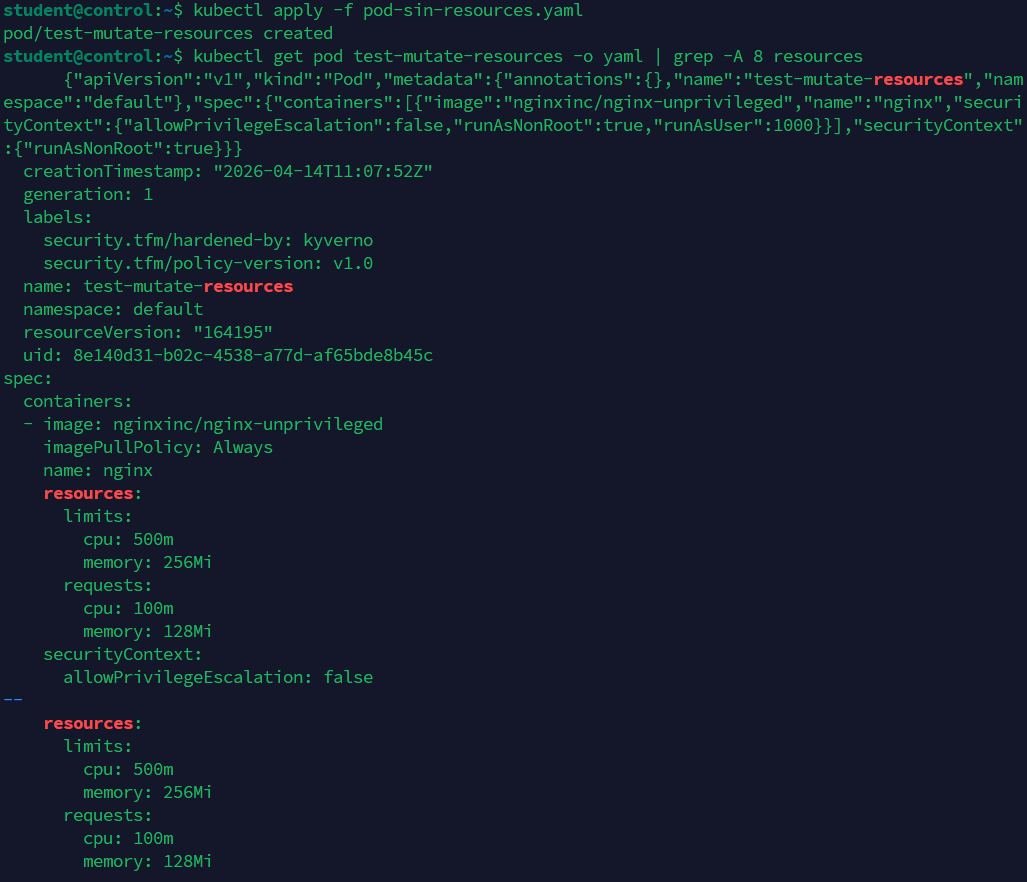
\includegraphics[width=0.95\linewidth]{kyverno/test4.png}
\caption{P4: inyección automática de \texttt{resources.requests} y \texttt{resources.limits}}
\label{fig:test4}
\end{figure}

Resulta especialmente significativo que la salida muestre también los labels \texttt{security.tfm/hardened-by: kyverno} y \texttt{security.tfm/policy-version: v1.0}, evidencia de que P7 (descrita en la Sección~6.4.4) también ha actuado sobre el mismo recurso en el mismo ciclo de admisión. Esto demuestra que las múltiples políticas de mutación se aplican de forma coordinada sobre cada objeto en un único paso de admisión.

\subsection{Política P5: \texttt{add-default-securitycontext}}

La quinta política inyecta un \texttt{securityContext} seguro en todos los contenedores que no lo especifiquen:

\begin{center}
\begin{minipage}{0.88\linewidth}
\begin{verbatim}
apiVersion: kyverno.io/v1
kind: ClusterPolicy
metadata:
  name: add-default-securitycontext
spec:
  rules:
  - name: add-container-security-context
    match:
      any:
      - resources:
          kinds:
          - Pod
    mutate:
      patchStrategicMerge:
        spec:
          containers:
          - (name): "*"
            securityContext:
              allowPrivilegeEscalation: false
              capabilities:
                drop:
                - ALL
\end{verbatim}
\end{minipage}
\end{center}

Esta política implementa dos controles de \textit{hardening} críticos de forma automática. El primero, \texttt{allowPrivilegeEscalation: false}, activa el flag \texttt{no\_new\_privs} del kernel, impidiendo la escalada de privilegios a través de binarios SUID, tal como se explicó en la Sección~6.3.2. Aquí la política actúa de forma \textit{proactiva} —inyectando la configuración segura antes de que llegue a la validación— en contraste con P2, que actúa de forma \textit{reactiva} rechazando la declaración explícita del valor inseguro.

El segundo control, \texttt{capabilities.drop: ALL}, elimina el conjunto completo de Linux capabilities heredadas por defecto por los contenedores en Kubernetes. Por defecto, y sin configuración adicional, un contenedor hereda un subconjunto de capabilities que incluye \texttt{NET\_RAW} (permite construir paquetes raw, facilitando ataques de red como spoofing), \texttt{MKNOD} (permite crear dispositivos de bloque), \texttt{CHOWN} (permite cambiar la propiedad de ficheros), entre otras. Estas capabilities son raramente necesarias para el funcionamiento de una aplicación típica y amplían innecesariamente la superficie de ataque. Al eliminarlas todas por defecto, se fuerza a los desarrolladores a declarar explícitamente las capabilities que sus aplicaciones realmente necesitan.

Esta política es el ejemplo más representativo del concepto de \textit{auto-hardening}: el desarrollador puede desplegar un pod con configuración mínima sin conocimiento profundo de los campos de seguridad de Kubernetes, y la plataforma garantiza que el pod resultante cumple con un perfil de seguridad sólido.

La prueba despliega un pod con un \texttt{securityContext} definido solo a nivel de pod (no a nivel de contenedor). La Figura~\ref{fig:test5} muestra el resultado de la inspección del pod creado: el \texttt{securityContext} a nivel de contenedor contiene \texttt{allowPrivilegeEscalation: false}, \texttt{capabilities.drop: [ALL]} y también \texttt{readOnlyRootFilesystem: true} —inyectado por P6 en el mismo ciclo de admisión.

\begin{figure}[H]
\centering
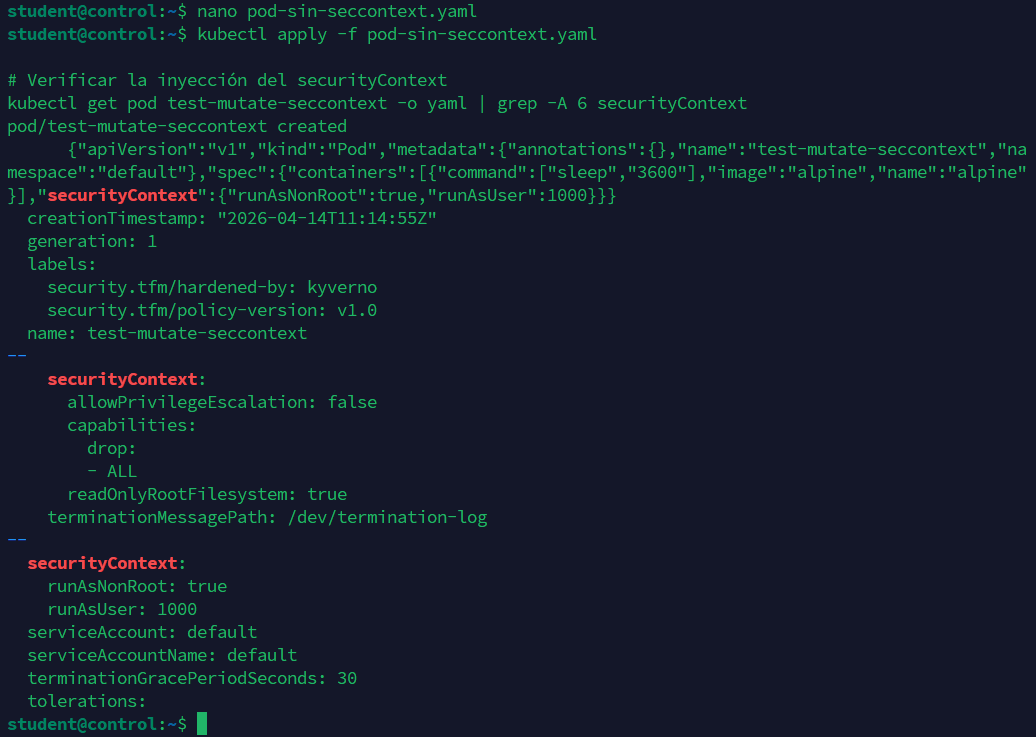
\includegraphics[width=0.95\linewidth]{kyverno/test5.png}
\caption{P5: inyección automática de \texttt{allowPrivilegeEscalation} y \texttt{capabilities.drop}}
\label{fig:test5}
\end{figure}

\subsection{Política P6: \texttt{add-readonly-rootfs}}

La sexta política fuerza el sistema de ficheros raíz de todos los contenedores a modo de solo lectura:

\begin{center}
\begin{minipage}{0.88\linewidth}
\begin{verbatim}
apiVersion: kyverno.io/v1
kind: ClusterPolicy
metadata:
  name: add-readonly-rootfs
spec:
  rules:
  - name: add-readonly-filesystem
    match:
      any:
      - resources:
          kinds:
          - Pod
    mutate:
      patchStrategicMerge:
        spec:
          containers:
          - (name): "*"
            securityContext:
              readOnlyRootFilesystem: true
\end{verbatim}
\end{minipage}
\end{center}

La justificación técnica de este control radica en el comportamiento habitual de los atacantes tras comprometer un contenedor: la mayoría de las técnicas de post-explotación —descarga de reverse shells, instalación de criptominers, ejecución de herramientas de reconocimiento— requieren escribir ficheros en el sistema de ficheros del contenedor. Un filesystem raíz de solo lectura hace que todos estos intentos fallen inmediatamente, conteniendo el radio de impacto de la intrusión.

La prueba verifica este efecto en dos pasos, ambos mostrados en la Figura~\ref{fig:test6}. Primero, se comprueba mediante la salida de \texttt{kubectl get pod -o yaml} que el campo \texttt{readOnlyRootFilesystem: true} ha sido inyectado. Segundo —y más significativo—, se ejecuta un comando dentro del contenedor que intenta crear un fichero en el directorio raíz:

\begin{center}
\begin{minipage}{0.88\linewidth}
\begin{verbatim}
kubectl exec test-mutate-seccontext -- touch /test-file
touch: /test-file: Read-only file system
command terminated with exit code 1
\end{verbatim}
\end{minipage}
\end{center}

\begin{figure}[H]
\centering
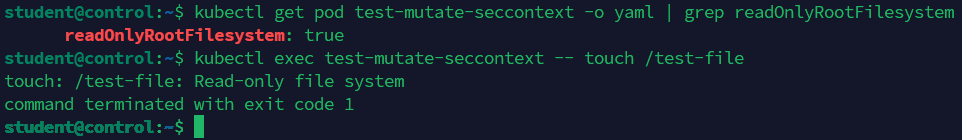
\includegraphics[width=0.90\linewidth]{kyverno/test6.png}
\caption{P6: verificación del filesystem de solo lectura en tiempo de ejecución}
\label{fig:test6}
\end{figure}

Este resultado es especialmente valioso: demuestra que la mutación aplicada por Kyverno en tiempo de admisión tiene un efecto real y verificable sobre el comportamiento del contenedor en tiempo de ejecución, no solo sobre el manifiesto almacenado en etcd.

Una limitación operativa conocida de esta política es que ciertas aplicaciones requieren escritura en directorios como \texttt{/tmp}, \texttt{/var/cache} o \texttt{/var/log}. La solución correcta —y la que se aplica en el propio pod integral de la Sección~6.6.2— consiste en montar un volumen de tipo \texttt{emptyDir} en los paths específicos que requieren escritura. Esta práctica no representa un debilitamiento de la política, sino una buena práctica de diseño que hace explícitas las necesidades de escritura de cada aplicación.

\subsection{Política P7: \texttt{add-default-labels}}

La séptima política inyecta etiquetas de trazabilidad en todos los pods procesados por el sistema:

\begin{center}
\begin{minipage}{0.88\linewidth}
\begin{verbatim}
apiVersion: kyverno.io/v1
kind: ClusterPolicy
metadata:
  name: add-default-labels
spec:
  rules:
  - name: add-security-labels
    match:
      any:
      - resources:
          kinds:
          - Pod
    mutate:
      patchStrategicMerge:
        metadata:
          labels:
            security.tfm/hardened-by: kyverno
            security.tfm/policy-version: "v1.0"
\end{verbatim}
\end{minipage}
\end{center}

Aunque menos obvia que las políticas de seguridad directa, esta política implementa una capacidad de observabilidad y trazabilidad relevante en entornos productivos. Los labels inyectados permiten identificar en todo momento qué pods han sido procesados por el sistema de políticas y con qué versión, facilitando la auditoría de cobertura y la detección de pods que pudieran haber evadido el proceso de admisión (por ejemplo, pods pre-existentes antes del despliegue de Kyverno). El campo \texttt{security.tfm/policy-version} actúa como un marcador de versión que permite correlacionar el perfil de seguridad aplicado con la versión de políticas vigente en el momento del despliegue.

La verificación mediante \texttt{kubectl get pods --show-labels}, mostrada en la Figura~\ref{fig:test7}, confirma que los labels están presentes en todos los pods activos en el namespace \texttt{default}.

\begin{figure}[H]
\centering
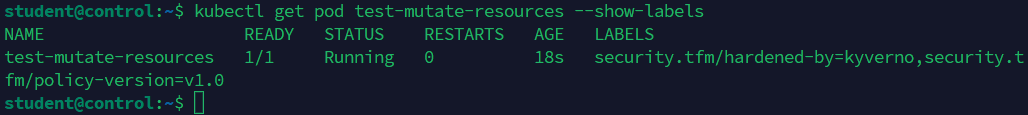
\includegraphics[width=0.90\linewidth]{kyverno/test7.png}
\caption{P7: labels de trazabilidad inyectados automáticamente en los pods}
\label{fig:test7}
\end{figure}

% ─────────────────────────────────────────────
\section{Política de generación}
% ─────────────────────────────────────────────

\subsection{Política P8: \texttt{generate-networkpolicy-metadata}}

La octava política demuestra el tercer tipo de acción disponible en Kyverno —\textit{generate}— y no tiene equivalente funcional en OPA Gatekeeper. A diferencia de las políticas anteriores, que actúan sobre recursos que ya están siendo creados, esta política reacciona ante la creación de un recurso de tipo \texttt{Namespace} y genera automáticamente un recurso derivado: una NetworkPolicy que bloquea el acceso al servicio de metadatos de instancia cloud (IMDS):

\begin{center}
\begin{minipage}{0.88\linewidth}
\begin{verbatim}
apiVersion: kyverno.io/v1
kind: ClusterPolicy
metadata:
  name: generate-networkpolicy-metadata
spec:
  rules:
  - name: block-metadata-service
    match:
      any:
      - resources:
          kinds:
          - Namespace
    generate:
      apiVersion: networking.k8s.io/v1
      kind: NetworkPolicy
      name: block-cloud-metadata
      namespace: "{{request.object.metadata.name}}"
      synchronize: true
      data:
        spec:
          podSelector: {}
          policyTypes:
          - Egress
          egress:
          - to:
            - ipBlock:
                cidr: 0.0.0.0/0
                except:
                - 169.254.169.254/32
\end{verbatim}
\end{minipage}
\end{center}

La NetworkPolicy generada permite todo el tráfico de salida (\texttt{cidr: 0.0.0.0/0}) excepto hacia la dirección \texttt{169.254.169.254/32}. Esta IP corresponde al IMDS presente en los principales proveedores cloud (AWS, GCP, Azure) y accesible desde cualquier instancia sin autenticación previa a través de HTTP. Un atacante que comprometa un pod en un entorno cloud puede realizar una solicitud a \texttt{http://169.254.169.254/latest/meta-data/} para obtener credenciales IAM temporales, tokens de servicio y configuración de red de la instancia subyacente, permitiendo la escalada desde el pod hasta la cuenta cloud. Este vector fue utilizado de forma documentada en el incidente de Capital One en 2019, donde un atacante aprovechó una vulnerabilidad SSRF para acceder al IMDS y obtener credenciales con las que exfiltrar datos de S3 \cite{capitalone2019}.

El campo \texttt{synchronize: true} activa el mecanismo de \textit{drift protection} del Background Controller de Kyverno: si la NetworkPolicy generada es modificada o eliminada, Kyverno la restaura automáticamente a su estado original.

La primera prueba, mostrada en la Figura~\ref{fig:test8}, demuestra la generación automática: se crea el namespace \texttt{test-networkpolicy} y, 9 segundos después, la NetworkPolicy \texttt{block-cloud-metadata} existe en dicho namespace sin que haya sido aplicada manualmente. La descripción detallada del recurso generado confirma que Kyverno ha añadido los labels de trazabilidad (\texttt{app.kubernetes.io/managed-by=kyverno}, \texttt{generate.kyverno.io/policy-name=generate-networkpolicy-metadata}) y que la regla de egress bloquea exclusivamente la IP \texttt{169.254.169.254/32}.

\begin{figure}[H]
\centering
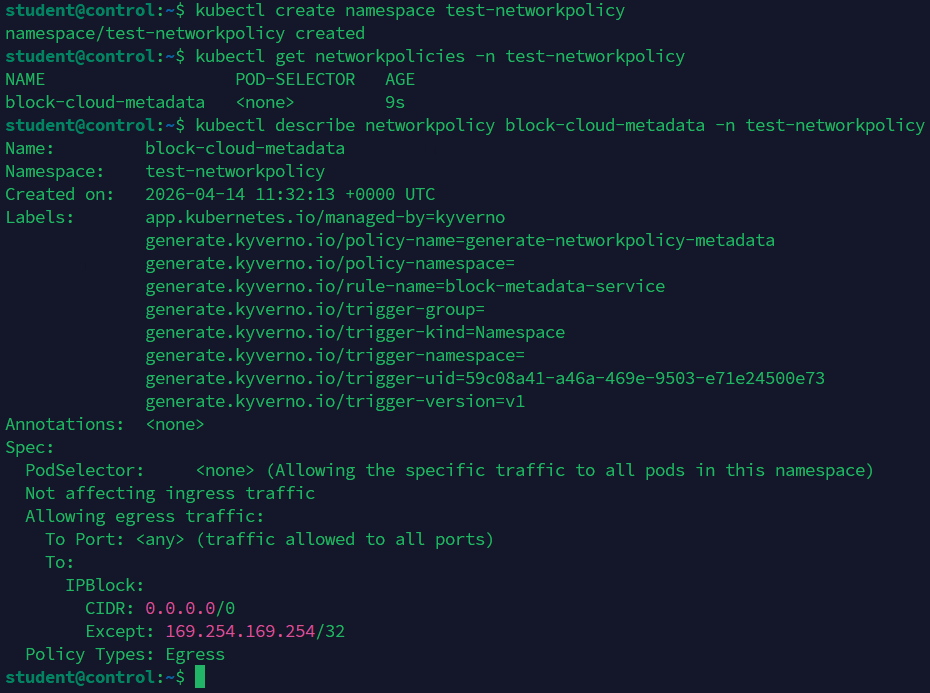
\includegraphics[width=0.95\linewidth]{kyverno/test8.png}
\caption{P8: NetworkPolicy generada automáticamente al crear el namespace}
\label{fig:test8}
\end{figure}

La segunda prueba, mostrada en la Figura~\ref{fig:test9}, demuestra el mecanismo de \textit{drift protection}: la NetworkPolicy es eliminada manualmente mediante \texttt{kubectl delete}, y 57 segundos después ha sido regenerada automáticamente por el Background Controller de Kyverno, sin intervención humana.

\begin{figure}[H]
\centering
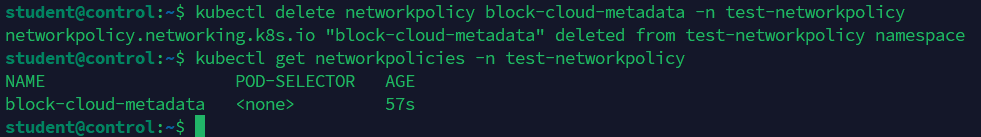
\includegraphics[width=0.90\linewidth]{kyverno/test9.png}
\caption{P8: drift protection — NetworkPolicy regenerada 57 segundos tras su eliminación manual}
\label{fig:test9}
\end{figure}

Este comportamiento ilustra una diferencia fundamental respecto a OPA Gatekeeper, que carece de soporte nativo para la generación de recursos y por tanto no puede implementar este patrón de protección continua.

% ─────────────────────────────────────────────
\section{Consideraciones operativas y lecciones aprendidas}
% ─────────────────────────────────────────────

\subsection{Exclusión de namespaces de infraestructura}

Durante las fases iniciales de la implementación, las políticas de validación generaban infracciones sobre los propios componentes del clúster. En particular, la política P1 (\texttt{disallow-root}) marcaba como no conformes ciertos pods del namespace \texttt{kube-system} que ejecutan como root por requisito de su función. Paralelamente, la primera versión de la política P3 (\texttt{restrict-image-registries}) no incluía el patrón \texttt{ghcr.io/*} en la lista de registros permitidos, lo que generaba PolicyViolations sobre los propios controladores de Kyverno, cuyas imágenes se distribuyen a través de \texttt{ghcr.io/kyverno/}.

La solución aplicada fue doble. Por un lado, se añadió \texttt{ghcr.io/*} a la lista de registros autorizados en P3, corrigiendo el problema de forma estructural. Por otro, el uso de \texttt{ClusterPolicy} con scope irrestricto se revisó para excluir los namespaces de infraestructura (\texttt{kyverno}, \texttt{kube-system}) en aquellas políticas donde su aplicación no es pertinente. Esta es una práctica estándar en despliegues productivos de Kyverno, donde las políticas de seguridad deben diseñarse con consciencia de los componentes del sistema que las ejecutan. La Figura~\ref{fig:rules-aplicadas} muestra el estado final del clúster con las ocho políticas en estado \texttt{Ready}.

\begin{figure}[H]
\centering
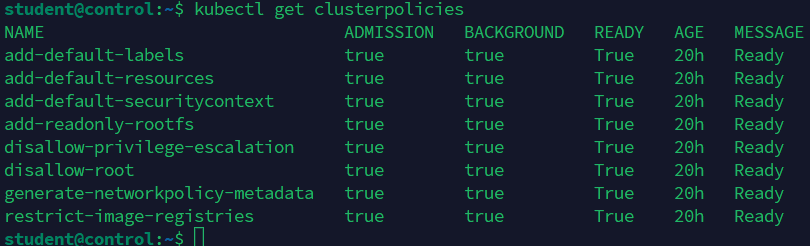
\includegraphics[width=0.95\linewidth]{kyverno/rulesAplicadas.png}
\caption{Las ocho ClusterPolicies en estado \texttt{Ready} tras el despliegue completo}
\label{fig:rules-aplicadas}
\end{figure}

\subsection{Prueba integral de auto-hardening}

La prueba más representativa del trabajo consiste en desplegar un pod con una configuración deliberadamente mínima y verificar que el conjunto completo de políticas de mutación lo transforma automáticamente en un pod con perfil de seguridad completo. El manifiesto inicial del pod, mostrado en la Figura~\ref{fig:pod-seguro-yaml}, contiene únicamente los campos estrictamente necesarios para que funcione: imagen, usuario de ejecución y un volumen \texttt{emptyDir} montado en \texttt{/tmp} para satisfacer la política P6 de filesystem de solo lectura.

\begin{figure}[H]
\centering
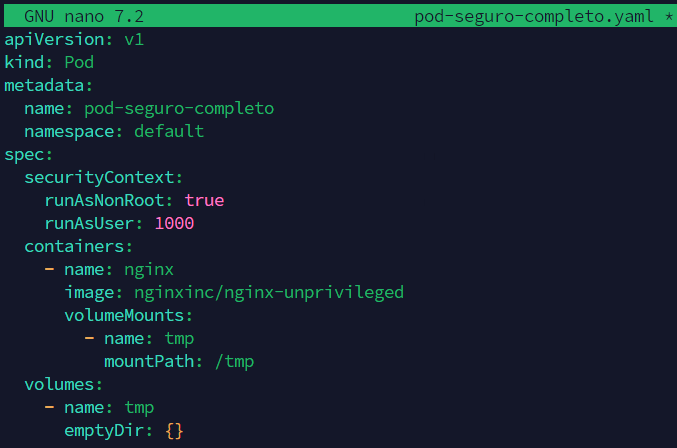
\includegraphics[width=0.65\linewidth]{kyverno/pod-seguro-completo.png}
\caption{Manifiesto mínimo del pod utilizado en la prueba integral}
\label{fig:pod-seguro-yaml}
\end{figure}

Tras el despliegue, la inspección del pod mediante \texttt{kubectl get pod pod-seguro-completo -o yaml} devuelve el objeto completo tal como ha sido persistido en etcd después del paso por los webhooks de Kyverno. Las Figuras~\ref{fig:test10-1} y~\ref{fig:test10-2} muestran el resultado en su totalidad.

\begin{figure}[H]
\centering
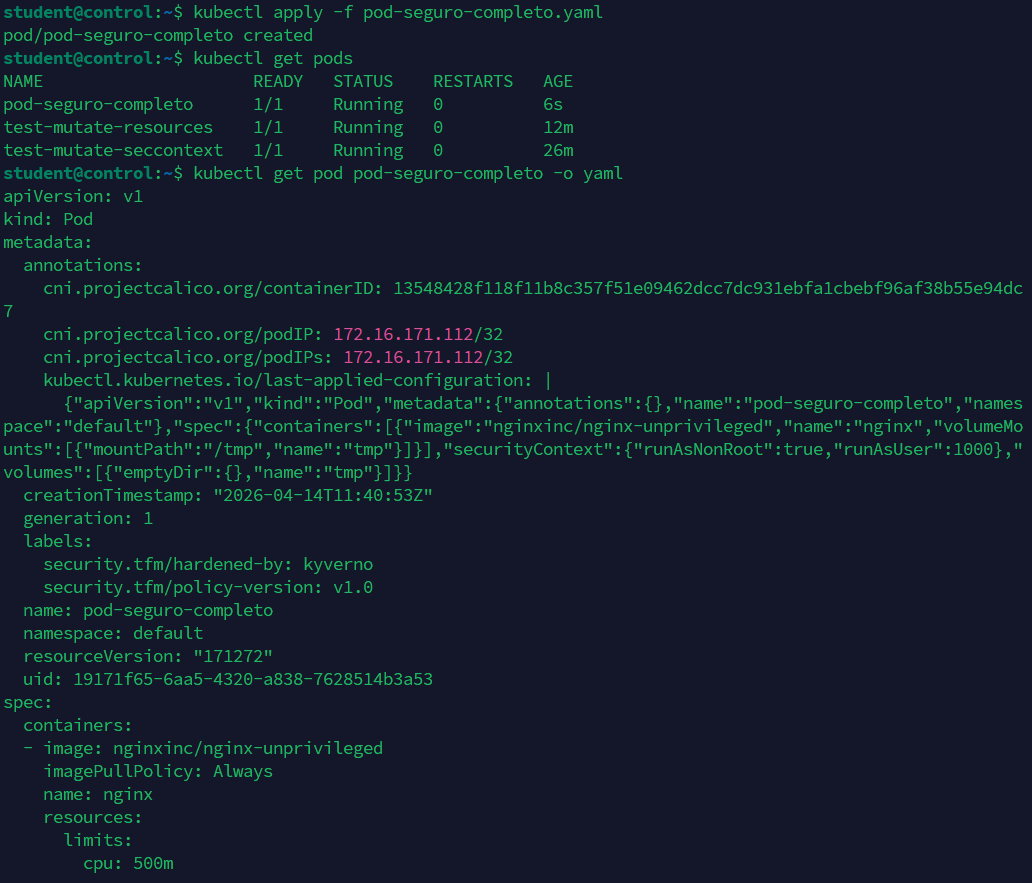
\includegraphics[width=0.95\linewidth]{kyverno/test10-1.png}
\caption{Prueba integral (parte 1): metadata y spec inicial del pod tras la admisión}
\label{fig:test10-1}
\end{figure}

\begin{figure}[H]
\centering
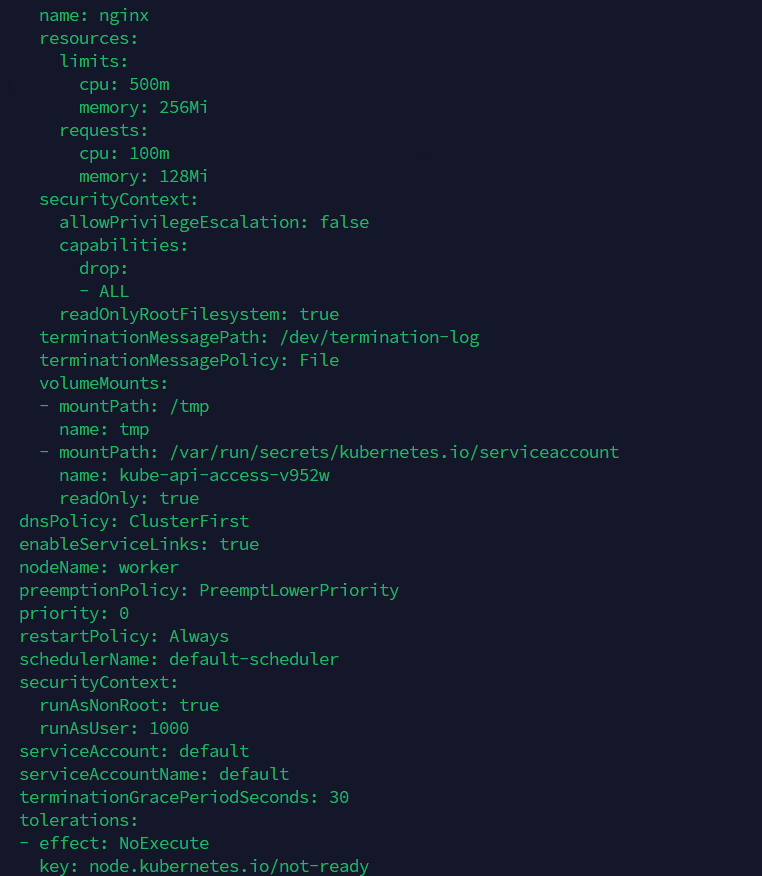
\includegraphics[width=0.85\linewidth]{kyverno/test10-2.png}
\caption{Prueba integral (parte 2): perfil de seguridad completo inyectado por Kyverno}
\label{fig:test10-2}
\end{figure}

El análisis del objeto persistido confirma la presencia de todos los campos inyectados por las cuatro políticas de mutación activas:

\begin{itemize}
    \item \textbf{P4 — resources:} \texttt{limits} (cpu: 500m, memory: 256Mi) y \texttt{requests} (cpu: 100m, memory: 128Mi) inyectados automáticamente.
    \item \textbf{P5 — securityContext:} \texttt{allowPrivilegeEscalation: false} y \texttt{capabilities.drop: [ALL]} inyectados en el contenedor.
    \item \textbf{P6 — readOnlyRootFilesystem:} \texttt{readOnlyRootFilesystem: true} inyectado. El volumen \texttt{emptyDir} montado en \texttt{/tmp} permite la escritura en ese path específico sin comprometer el aislamiento del filesystem.
    \item \textbf{P7 — labels:} \texttt{security.tfm/hardened-by: kyverno} y \texttt{security.tfm/policy-version: v1.0} presentes en los metadata del pod.
\end{itemize}

Adicionalmente, las anotaciones de Calico confirman que el pod ha sido asignado la IP \texttt{172.16.171.112} dentro del espacio de direccionamiento \texttt{172.16.0.0/16}, y que ha sido programado en el nodo \texttt{worker} (\texttt{nodeName: worker}), tal como corresponde a la arquitectura de dos nodos del laboratorio.

Esta prueba constituye la evidencia empírica directa de la tesis central del trabajo: un desarrollador puede definir un pod con los campos mínimos necesarios para su función y obtener, de forma completamente transparente y sin conocimiento de los detalles de seguridad de Kubernetes, un pod correctamente securizado que cumple con el perfil de seguridad definido por la organización.

\subsection{El orden mutación-validación verificado empíricamente}

Durante las pruebas se observó un comportamiento que ilustra empíricamente el orden de ejecución de los webhooks descrito teóricamente en la Sección~5.3.2. En una sesión de prueba, se intentó desplegar un pod con \texttt{allowPrivilegeEscalation: true} declarado de forma explícita mientras P5 y P2 estaban activas simultáneamente. El pod fue creado con éxito, pese a que P2 declara en modo \texttt{Enforce} que \texttt{allowPrivilegeEscalation: false} es obligatorio.

La causa es precisa: P5 (mutating webhook) se ejecutó antes que P2 (validating webhook) y sobreescribió el valor \texttt{true} declarado en el manifiesto por \texttt{false}, de modo que cuando P2 evaluó el recurso, ya contenía el valor conforme. El \texttt{patchStrategicMerge} de P5 sobreescribe el campo incluso cuando el desarrollador lo ha declarado explícitamente con un valor inseguro.

Este comportamiento fue verificado deshabilitando temporalmente P5 y aplicando el mismo pod: en ausencia de la mutación, P2 rechazó correctamente la solicitud con el mensaje \textit{"Privilege escalation is not allowed"}. Al restaurar P5, el pod volvió a ser admitido con el valor mutado. Este experimento confirma empíricamente que, en el diseño adoptado, la mutación tiene \textit{precedencia absoluta} sobre la validación, y que las políticas de validación complementan pero no sustituyen a las de mutación como mecanismo de seguridad principal.

% ─────────────────────────────────────────────
\section{Policy Reports: auditoría de cumplimiento}
% ─────────────────────────────────────────────

El Reports Controller de Kyverno genera automáticamente recursos \texttt{PolicyReport} (con alcance de namespace) y \texttt{ClusterPolicyReport} (con alcance de clúster) que consolidan los resultados de la evaluación de todas las políticas sobre todos los recursos del sistema. Estos informes constituyen el mecanismo de auditoría de cumplimiento nativo del sistema y permiten responder de forma centralizada a la pregunta: ¿qué recursos del clúster están en conformidad con las políticas de seguridad?

La Figura~\ref{fig:clusterpolicyreports} muestra el \texttt{ClusterPolicyReport} generado para el namespace \texttt{test-networkpolicy}: el recurso de tipo \texttt{Namespace} con ese nombre ha superado la evaluación de la política P8 (\texttt{generate-networkpolicy-metadata}), con un resultado de 1 PASS y 0 FAIL.

\begin{figure}[H]
\centering
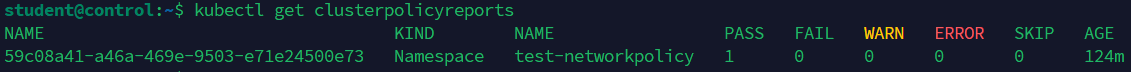
\includegraphics[width=0.95\linewidth]{kyverno/kubectl get clusterpolicyreports.png}
\caption{ClusterPolicyReport: evaluación de la política de generación sobre el namespace de prueba}
\label{fig:clusterpolicyreports}
\end{figure}

La Figura~\ref{fig:policyreports} muestra los \texttt{PolicyReport} del namespace \texttt{default}, uno por cada pod activo. Los tres pods — \texttt{pod-seguro-completo}, \texttt{test-mutate-resources} y \texttt{test-mutate-seccontext} — registran 7 PASS y 0 FAIL.

\begin{figure}[H]
\centering
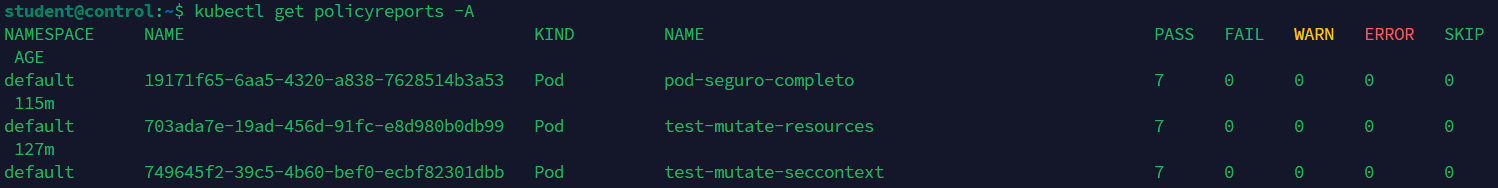
\includegraphics[width=0.95\linewidth]{kyverno/kubectl get policyreports -A.png}
\caption{PolicyReports del namespace \texttt{default}: 7 PASS por pod, 0 infracciones}
\label{fig:policyreports}
\end{figure}

El valor 7 corresponde exactamente al número de políticas que evalúan recursos de tipo \texttt{Pod} (P1 a P7), confirmando que todos los pods activos en el clúster cumplen la totalidad de las políticas desplegadas. La política P8 no aparece en estos informes porque su alcance es sobre recursos de tipo \texttt{Namespace}, no \texttt{Pod}, y sus resultados se reflejan en los \texttt{ClusterPolicyReport} de la Figura~\ref{fig:clusterpolicyreports}.

Estos informes demuestran que el sistema implementado no solo actúa en tiempo de admisión, sino que proporciona visibilidad continua sobre el estado de cumplimiento del clúster — un requisito fundamental en entornos DevSecOps orientados a la auditoría y el cumplimiento normativo.

\chapter{Integración GitOps con ArgoCD}

El presente capítulo documenta la implementación de la capa de Despliegue Continuo del entorno DevSecOps, materializada mediante ArgoCD como controlador GitOps. Hasta este punto, las políticas de Kyverno han sido gestionadas mediante \texttt{kubectl apply} directo, lo que implica que el estado del clúster y el estado declarado en los manifiestos no están vinculados de forma continua: cualquier modificación manual en el clúster puede divergir del estado deseado sin que ningún mecanismo lo detecte ni corrija. Este capítulo implementa el plano de sincronización continua anunciado en la Sección~5.1, cerrando la arquitectura DevSecOps con la capa que conecta el repositorio Git como fuente única de verdad con el estado real del clúster.

El capítulo se organiza en seis secciones. La primera describe el diseño del repositorio GitOps y la decisión sobre su estructura. La segunda documenta el despliegue de ArgoCD en el clúster, incluyendo una incidencia técnica relevante durante la instalación. La tercera cubre la creación de la \texttt{Application} que pone las políticas de Kyverno bajo gestión declarativa, y la cuarta documenta un hallazgo técnico sobre la fricción entre los defaults inyectados por Kyverno y el motor de comparación de ArgoCD. La quinta sección recoge las tres pruebas de \textit{drift protection} que demuestran empíricamente la tesis de complementariedad ArgoCD\,+\,Kyverno del Capítulo~5. La sexta sección extiende la arquitectura GitOps a una carga de trabajo real, y el capítulo concluye con un análisis técnico de la interacción entre los \textit{mutating webhooks} de Kyverno y el motor de comparación de ArgoCD, abordando directamente el riesgo de \textit{drift} permanente advertido por la documentación oficial. La integración con el plano de Integración Continua, que materializará el patrón de dos repositorios descrito teóricamente en la Sección~5.1, se aborda en el Capítulo~8 mediante la incorporación del pipeline de GitHub Actions.

% ─────────────────────────────────────────────
\section{Diseño del repositorio GitOps}
% ─────────────────────────────────────────────

El diseño del repositorio GitOps requiere una decisión arquitectónica previa: el número de repositorios que estructurarán el sistema. La Sección~5.1 describió teóricamente el \textit{patrón de dos repositorios} —uno para el código fuente de la aplicación y otro para la configuración de Kubernetes— como solución habitual en entornos productivos. En el alcance de este capítulo, donde aún no se ha incorporado el pipeline de Integración Continua, se trabaja con un único repositorio —denominado \texttt{tfm-gitops}— que contiene las políticas de Kyverno y los manifiestos de la aplicación demo, organizados mediante carpetas que preservan la separación conceptual entre planos. Esta estructura se ampliará en el Capítulo~8 con la introducción del segundo repositorio (\texttt{tfm-demo-app}), que albergará el código fuente y el Dockerfile de la aplicación. El pipeline de Integración Continua construirá la imagen desde ese segundo repositorio y actualizará el tag de imagen en \texttt{tfm-gitops}, materializando el patrón completo de dos repositorios anunciado en la arquitectura.

La estructura final del repositorio, visible en la Figura~\ref{fig:repo-estructura}, refleja tres planos funcionales independientes:

\begin{figure}[htbp]
\centering
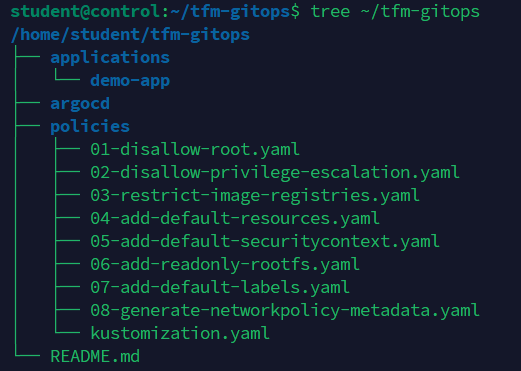
\includegraphics[width=0.70\linewidth]{actions/bloque1_estructuraInicial.png}
\caption{Estructura del repositorio \texttt{tfm-gitops} con separación por planos funcionales}
\label{fig:repo-estructura}
\end{figure}

\begin{itemize}
  \item \texttt{policies/}: contiene los ocho manifiestos de \texttt{ClusterPolicy} (P1--P8) y el fichero \texttt{kustomization.yaml} que los agrupa.
  \item \texttt{applications/demo-app/}: contiene los manifiestos de la carga de trabajo demostrativa (Namespace, Deployment, Service) y su propio \texttt{kustomization.yaml}.
  \item \texttt{argocd/}: contiene los manifiestos de tipo \texttt{Application} que definen cómo ArgoCD debe gestionar cada uno de los planos anteriores.
\end{itemize}

El fichero \texttt{kustomization.yaml} de la carpeta \texttt{policies/} juega un papel central en la integración con ArgoCD. Kustomize \cite{kustomize_docs} es un mecanismo de agrupación nativo de Kubernetes que ArgoCD reconoce automáticamente: al apuntar una \texttt{Application} a un directorio que contiene un \texttt{kustomization.yaml}, ArgoCD renderiza todos los recursos listados en él y los gestiona como una unidad lógica. Esto evita la necesidad de referenciar cada fichero de política individualmente en la configuración de ArgoCD. La Figura~\ref{fig:kustomization} muestra el contenido del fichero, que lista los ocho manifiestos en orden correlativo.

\begin{figure}[H]
\centering
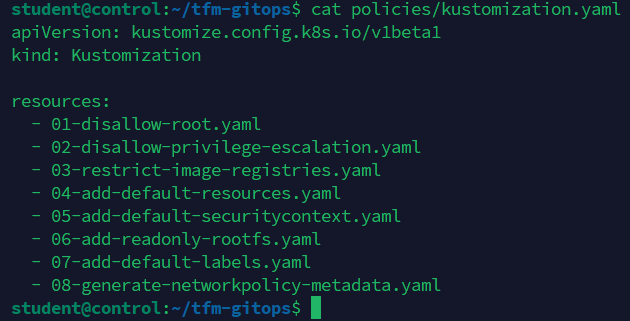
\includegraphics[width=0.75\linewidth]{actions/bloque1_kustomization.png}
\caption{Fichero \texttt{kustomization.yaml} de la carpeta \texttt{policies/} con las ocho políticas}
\label{fig:kustomization}
\end{figure}

% ─────────────────────────────────────────────
\section{Despliegue de ArgoCD}
% ─────────────────────────────────────────────

ArgoCD se instala en el clúster aplicando los manifiestos oficiales en el namespace dedicado \texttt{argocd}:

\begin{lstlisting}
kubectl create namespace argocd
kubectl apply -n argocd -f https://raw.githubusercontent.com/argoproj/argo-cd/stable/manifests/install.yaml
\end{lstlisting}

\subsection{Incidencia durante la instalación: límite de anotaciones en los CRDs}

Durante la primera ejecución del comando anterior se produjo un error que impidió el registro del CRD \texttt{ApplicationSet}:

\begin{lstlisting}
The ApplicationSet "applicationsets.argoproj.io" is invalid:
metadata.annotations: Too long: may not be more than 262144 bytes
\end{lstlisting}

La causa raíz de este error reside en el mecanismo de \textit{client-side apply} utilizado por defecto por \texttt{kubectl apply}: al aplicar un recurso, \texttt{kubectl} serializa el manifiesto completo y lo almacena en la anotación \texttt{kubectl.kubernetes.io/\allowbreak{}last-applied-configuration} del objeto. El esquema OpenAPI del CRD \texttt{ApplicationSet} supera el límite de 256~KB impuesto por Kubernetes para el valor de una anotación individual, lo que hace imposible completar la operación mediante el mecanismo estándar.

La solución consiste en reinstalar los manifiestos usando \textit{server-side apply} \cite{kubernetes_ssa}, que delega la lógica de \textit{merge} al API Server en lugar de almacenarla en la anotación del cliente:

\begin{lstlisting}
kubectl apply -n argocd \
  -f https://raw.githubusercontent.com/argoproj/argo-cd/stable/manifests/install.yaml \
  --server-side --force-conflicts
\end{lstlisting}

El flag \texttt{-{}-force-conflicts} es necesario porque algunos campos de los manifiestos pudieron quedar en estado de \textit{field manager} inconsistente tras el primer intento parcialmente completado. Con \textit{server-side apply}, el campo \texttt{last-applied-configuration} no se utiliza y el CRD se registra correctamente independientemente del tamaño de su esquema.

\subsection{Verificación del despliegue}

Tras la reinstalación, la verificación del estado de los pods en el namespace \texttt{argocd} confirma que los siete componentes de ArgoCD están activos, como muestra la Figura~\ref{fig:argo-pods}.

\begin{figure}[H]
\centering
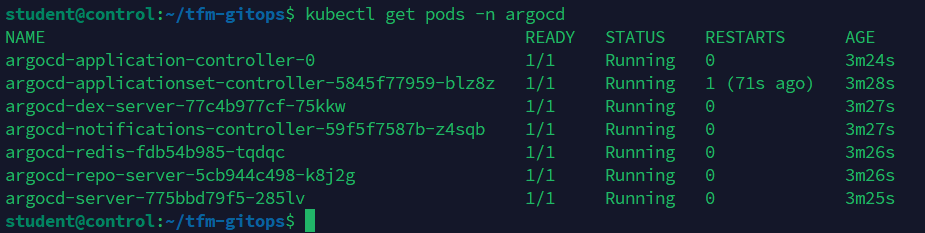
\includegraphics[width=0.95\linewidth]{actions/bloque2_verificaionPodsArgo.png}
\caption{Los siete componentes de ArgoCD en estado \texttt{Running} en el namespace \texttt{argocd}}
\label{fig:argo-pods}
\end{figure}

Los siete pods corresponden a los componentes descritos en la Sección~5.2.3: \texttt{application-cont\-roller} (reconciliación continua del estado del clúster), \texttt{applicationset-controller} (generación de \texttt{Application} a partir de plantillas), \texttt{dex-server} (autenticación federada), \texttt{notifications-controller} (alertas y notificaciones), \texttt{redis} (caché de estado interno), \texttt{repo-server} (clonado y renderizado de repositorios Git) y \texttt{server} (API y UI de ArgoCD).

La verificación de los CRDs registrados confirma que los tres tipos de recurso de ArgoCD están disponibles en el clúster, como se aprecia en la Figura~\ref{fig:argo-crds}.

\begin{figure}[H]
\centering
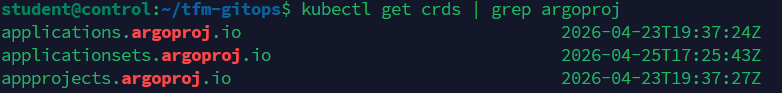
\includegraphics[width=0.85\linewidth]{actions/bloque2_CRDSregistrados.png}
\caption{CRDs de ArgoCD registrados en el clúster: \texttt{applications}, \texttt{applicationsets} y \texttt{appprojects}}
\label{fig:argo-crds}
\end{figure}

El \textit{dashboard} de ArgoCD (versión~3.3.8) es accesible a través del puerto \texttt{8080} del nodo de control mediante la exposición del servicio \texttt{argocd-server}. La Figura~\ref{fig:argo-dashboard} muestra el estado inicial de la interfaz antes de registrar ninguna \texttt{Application}.

\begin{figure}[htbp]
\centering
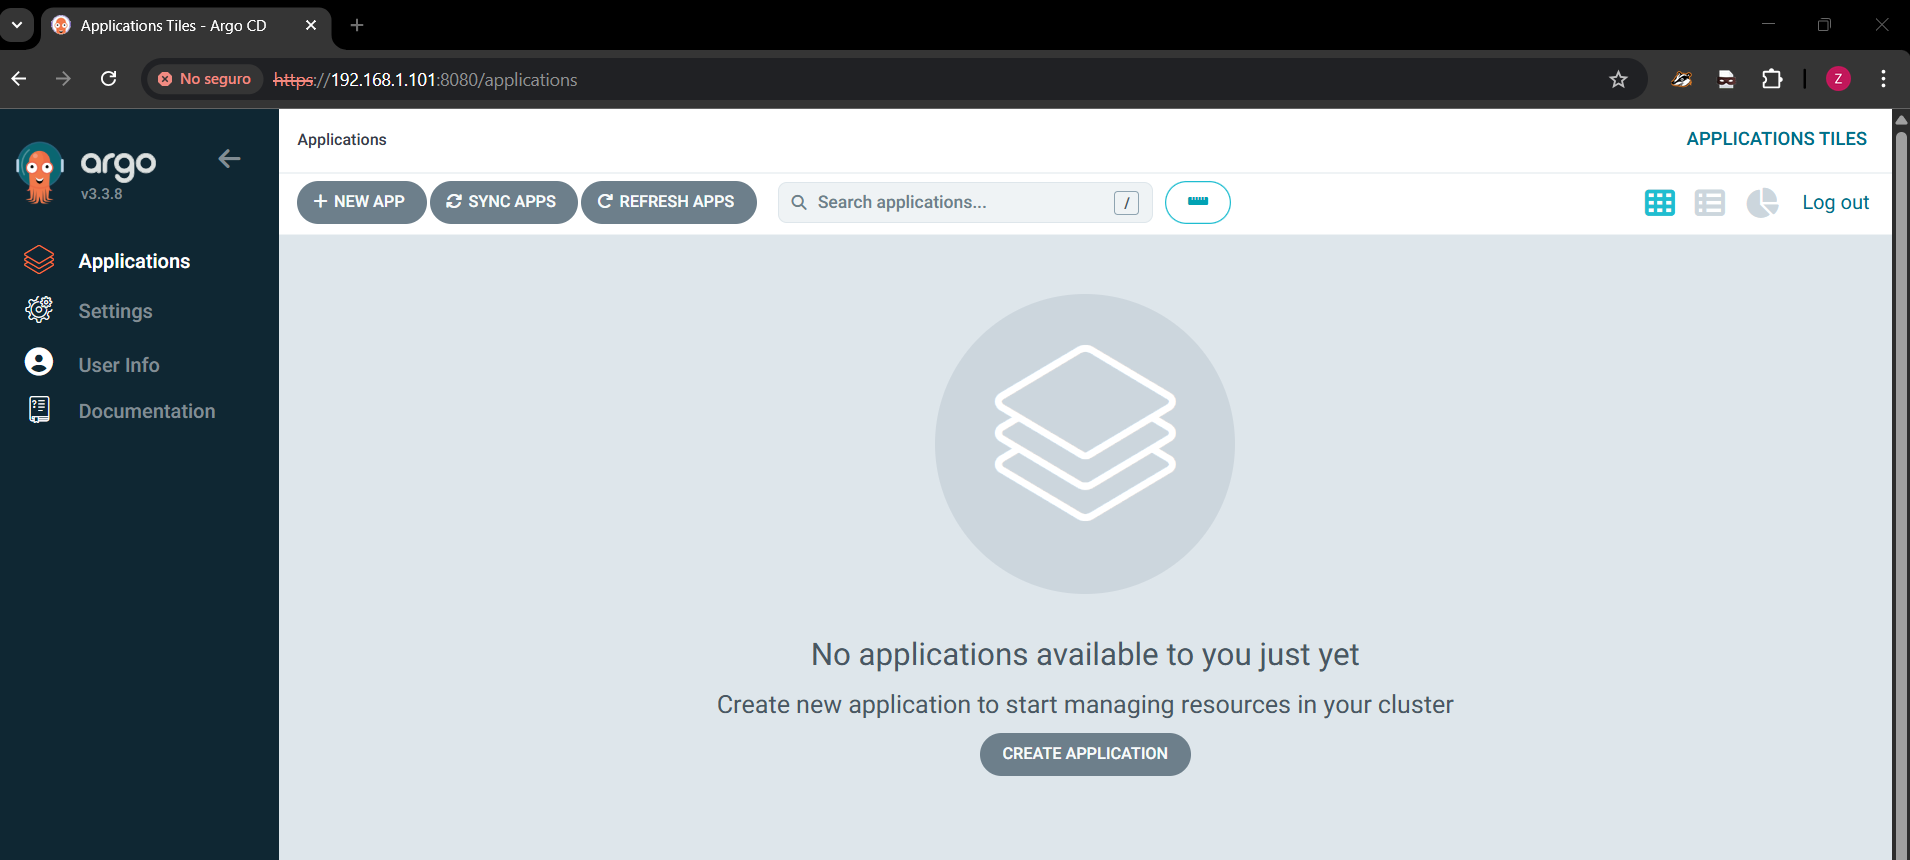
\includegraphics[width=0.95\linewidth]{actions/bloque2_dashboard.png}
\caption{Interfaz de ArgoCD v3.3.8 accesible en \texttt{https://192.168.1.101:8080}}
\label{fig:argo-dashboard}
\end{figure}

% ─────────────────────────────────────────────
\section{Application para las políticas de Kyverno}
\label{sec:app-policies}
% ─────────────────────────────────────────────

Una \texttt{Application} es el CRD central de ArgoCD \cite{argocd_docs}: representa la unidad mínima de gestión declarativa y encapsula tres elementos —la fuente Git de los manifiestos, el destino en el clúster donde deben desplegarse y la política de sincronización que define cómo y cuándo sincronizar. El manifiesto \texttt{app-policies.yaml}, mostrado en la Figura~\ref{fig:app-policies-yaml}, define la \texttt{Application} que pone las ocho políticas de Kyverno bajo gestión GitOps.

\begin{figure}[H]
\centering
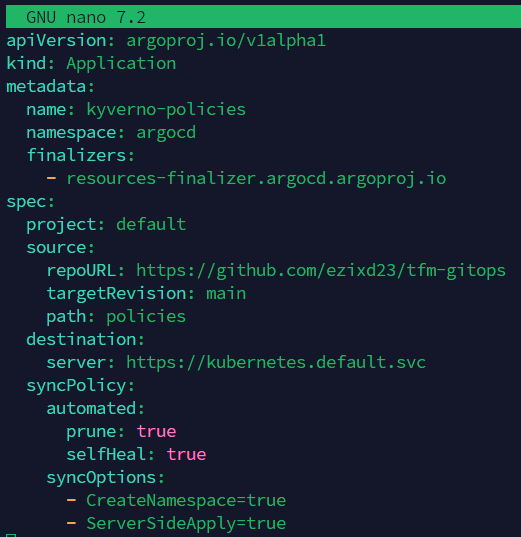
\includegraphics[width=0.70\linewidth]{actions/bloque3_app-policies.png}
\caption{Manifiesto \texttt{app-policies.yaml}: Application que gestiona las ClusterPolicies de Kyverno}
\label{fig:app-policies-yaml}
\end{figure}
\vspace{-\parskip}

Cada campo del manifiesto responde a una decisión técnica justificada:

\begin{itemize}
  \item \texttt{finalizers: resources-finalizer.\allowbreak{}argocd.argoproj.io}: activa el \textit{cascade delete}, de modo que al eliminar la \texttt{Application} de ArgoCD se eliminan también los recursos sincronizados en el clúster. Garantiza que no queden políticas huérfanas si la \texttt{Application} es suprimida.
  \item \texttt{automated.prune:\,true}: habilita la eliminación automática de recursos que existan en el clúster pero hayan sido eliminados de Git. Sin este campo, ArgoCD detectaría la divergencia pero no actuaría, requiriendo intervención manual.
  \item \texttt{automated.selfHeal:\,true}: activa la detección y reversión automática de modificaciones manuales realizadas directamente sobre los recursos del clúster. Este campo es el corazón de la tesis de complementariedad con Kyverno formulada en la Sección~5.2.3: mientras Kyverno protege los recursos generados (NetworkPolicies), ArgoCD protege las propias fuentes de esa generación (ClusterPolicies).
  \item \texttt{syncOptions.ServerSideApply:\,true}: delega el \textit{merge} de los recursos al API Server, evitando el problema de tamaño de anotaciones descrito en la sección anterior y siendo coherente con la instalación de los propios manifiestos de ArgoCD.
  \item \texttt{syncOptions.CreateNamespace:\,true}: permite a ArgoCD crear el namespace de destino si no existe, aunque en este caso el namespace \texttt{kyverno} ya está creado por la instalación previa de Kyverno.
\end{itemize}

\subsection{Proceso de despliegue y sincronización}

Antes de aplicar la \texttt{Application}, se eliminan del clúster las políticas previamente desplegadas mediante \texttt{kubectl apply} directo, de modo que el despliegue subsiguiente demuestre de forma inequívoca que ArgoCD es la única fuente de aprovisionamiento:

\begin{lstlisting}
kubectl delete clusterpolicies --all
kubectl apply -f ~/tfm-gitops/argocd/app-policies.yaml
\end{lstlisting}

La Figura~\ref{fig:app-policies-sync} muestra la secuencia de estados observada: inmediatamente tras la aplicación del manifiesto, la \texttt{Application} \texttt{kyverno-policies} aparece en estado \texttt{OutOfSync}~+~\texttt{Healthy}, lo que indica que ArgoCD ha detectado la divergencia entre el repositorio (que contiene las ocho políticas) y el clúster (que en ese momento no tiene ninguna). En el siguiente ciclo de reconciliación, ArgoCD sincroniza el estado y la \texttt{Application} transita a \texttt{Synced}~+~\texttt{Healthy}.

\begin{figure}[H]
\centering
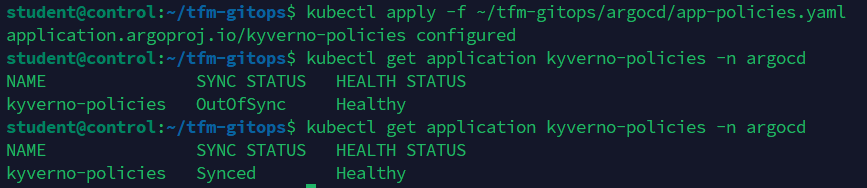
\includegraphics[width=0.95\linewidth]{actions/bloque3_aplicacionEstado.png}
\caption{Transición de estado \texttt{OutOfSync} → \texttt{Synced} tras el primer despliegue de \texttt{kyverno-policies}}
\label{fig:app-policies-sync}
\end{figure}

La verificación de que las ocho políticas han sido restauradas y están gestionadas por ArgoCD se realiza en dos pasos. El primero confirma el estado \texttt{Ready} de las ocho \texttt{ClusterPolicies}, como muestra la Figura~\ref{fig:policies-regeneradas}.

\begin{figure}[H]
\centering
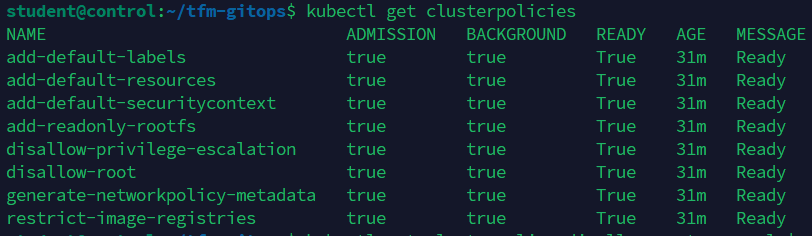
\includegraphics[width=0.95\linewidth]{actions/bloque3_policiesGeneradasDeNuevo.png}
\caption{Las ocho ClusterPolicies restauradas por ArgoCD en estado \texttt{Ready}}
\label{fig:policies-regeneradas}
\end{figure}
\vspace{-\parskip}

\begin{sloppypar}
El segundo paso verifica que el \textit{ownership} de cada política está establecido mediante la anotación de trazabilidad de ArgoCD. La Figura~\ref{fig:argo-anotacion} muestra que la política \texttt{disallow-root} contiene la anotación \path{argocd.argoproj.io/tracking-id:kyverno-policies:kyverno.io/ClusterPolicy:/disallow-root}, que establece inequívocamente que este recurso es gestionado por la \texttt{Application} \texttt{kyverno-policies}.
\end{sloppypar}

\begin{figure}[H]
\centering
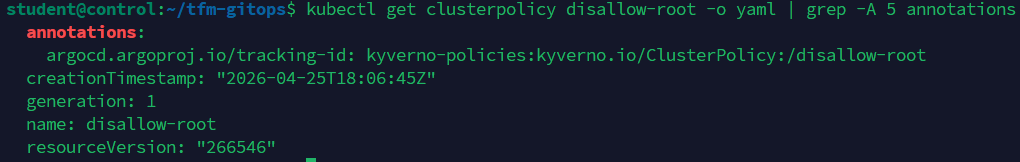
\includegraphics[width=0.95\linewidth]{actions/bloque3_anotacionesArgoCD.png}
\caption{Anotación de \textit{ownership} de ArgoCD en la ClusterPolicy \texttt{disallow-root}}
\label{fig:argo-anotacion}
\end{figure}
\vspace{-\parskip}

La interfaz gráfica de ArgoCD, mostrada en la Figura~\ref{fig:argo-arbol}, presenta el árbol de recursos sincronizados: la \texttt{Application} \texttt{kyverno-policies} con sus ocho \texttt{ClusterPolicy} dependientes, todas en estado \texttt{Synced}. El commit asociado a la última sincronización exitosa es visible en el panel de estado, confirmando que el origen de verdad es el repositorio Git.

\begin{figure}[H]
\centering
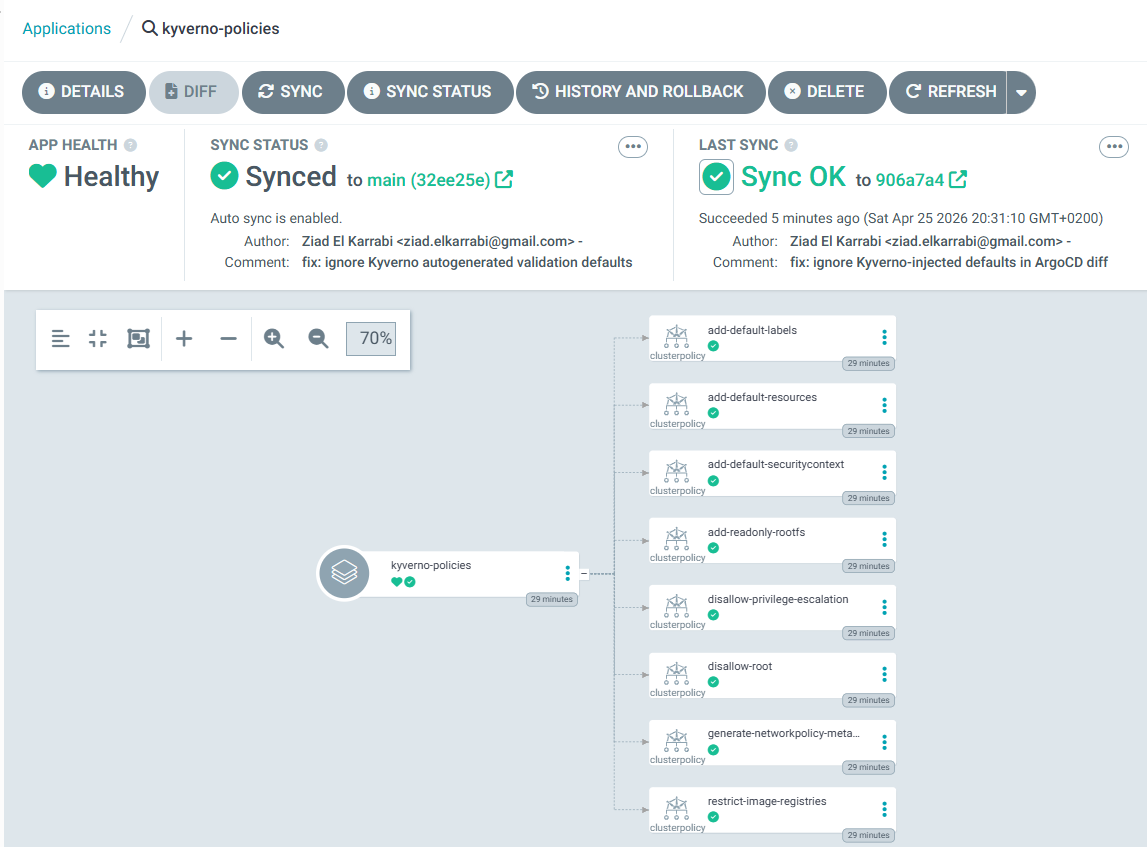
\includegraphics[width=0.95\linewidth]{actions/bloque3_arbolPolicies.png}
\caption{Vista de árbol en ArgoCD: ocho ClusterPolicies sincronizadas desde el repositorio Git}
\label{fig:argo-arbol}
\end{figure}
\vspace{-\parskip}

La prueba funcional end-to-end, mostrada en la Figura~\ref{fig:pod-bloqueado-argo}, confirma que las políticas gestionadas por ArgoCD son funcionalmente equivalentes a las desplegadas manualmente: el intento de crear un pod sin \texttt{runAsNonRoot} es rechazado por el webhook de Kyverno con el mismo mensaje que en las pruebas del Capítulo~6.

\begin{figure}[H]
\centering
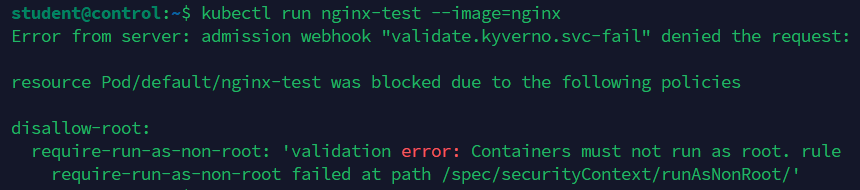
\includegraphics[width=0.90\linewidth]{actions/bloque3_podBloqueado.png}
\caption{Verificación end-to-end: pod inseguro bloqueado por las políticas gestionadas por ArgoCD}
\label{fig:pod-bloqueado-argo}
\end{figure}
\vspace{-\parskip}

% ─────────────────────────────────────────────
\section{Gestión del drift falso por defaults de Kyverno}
\label{sec:ignore-differences}
% ─────────────────────────────────────────────

Tras el primer despliegue exitoso de la \texttt{Application} \texttt{kyverno-policies}, se observó un comportamiento inesperado: la \texttt{Application} revertía periódicamente al estado \texttt{OutOfSync} pese a que ningún cambio había sido realizado ni en Git ni en el clúster. El análisis del diff de ArgoCD reveló la causa raíz: el propio Kyverno aplica un \textit{mutating webhook} sobre los recursos de tipo \texttt{ClusterPolicy} en el momento de su admisión, inyectando valores por defecto en campos que no están especificados en los manifiestos de Git. Los campos afectados incluyen \texttt{spec.\allowbreak{}validationFailureAction} (cuando no se declara explícitamente en alguna política), \texttt{spec.\allowbreak{}rules[*].skipBackgroundRequests} y \texttt{spec.\allowbreak{}rules[*].allowExistingViolations}.

Esta situación es un ejemplo de lo que la documentación de ArgoCD denomina \textit{drift falso} \cite{argocd_diffing}: el estado en el clúster difiere del estado en Git, pero la diferencia no es el resultado de una modificación no autorizada sino de un comportamiento interno del sistema. Desde la perspectiva de ArgoCD, el recurso en el clúster tiene campos adicionales o con valores distintos a los declarados en Git, lo que activa el mecanismo de \texttt{selfHeal} de forma innecesaria, creando un bucle de reconciliación inestable.

\subsection{Evaluación de las opciones de resolución}

Ante esta situación existen dos estrategias de resolución:

\begin{enumerate}
  \item \textbf{Añadir los valores por defecto a los manifiestos en Git}: declarar explícitamente en cada manifiesto los campos que Kyverno inyecta, de modo que el estado de Git y el estado en el clúster coincidan exactamente.
  \item \textbf{Configurar \texttt{ignoreDifferences} en la \texttt{Application}}: instruir a ArgoCD para que ignore ciertos campos al realizar la comparación, preservando los manifiestos de Git en su forma mínima.
\end{enumerate}

La primera opción tiene una desventaja operativa significativa: los valores por defecto inyectados por Kyverno son dependientes de la versión del motor. Una actualización de Kyverno que cambie los defaults existentes o añada nuevos campos requeriría actualizar todos los manifiestos de Git de forma sincronizada, creando un acoplamiento innecesario entre la versión del motor y los manifiestos de las políticas. Esta dependencia viola el principio de separación de responsabilidades que subyace al patrón GitOps: Git debe contener la \textit{intención} del operador, no un espejo exacto del estado interno del sistema.

La segunda opción, \texttt{ignoreDifferences} \cite{argocd_diffing}, permite expresar exactamente esta distinción: los campos ignorados son campos de gestión interna del motor, no atributos de la política declarada por el operador. Se adopta esta estrategia añadiendo el siguiente bloque al manifiesto \texttt{app-policies.yaml}:

\begin{lstlisting}
ignoreDifferences:
- group: kyverno.io
  kind: ClusterPolicy
  jqPathExpressions:
  - .spec.rules[] | .skipBackgroundRequests
  - .spec.rules[] | .allowExistingViolations
  - .spec.rules[] | .validate? | .allowExistingViolations?
  - .spec.validationFailureAction
\end{lstlisting}

Las expresiones \texttt{jqPathExpressions} utilizan la sintaxis de \texttt{jq} para referenciar los campos que deben excluirse de la comparación. El uso de \texttt{?.} en \texttt{.validate?} evita errores en reglas de tipo \textit{mutate} o \textit{generate} donde el campo \texttt{validate} no existe. Tras aplicar esta configuración y volver a sincronizar, la \texttt{Application} permanece de forma estable en estado \texttt{Synced}~+~\texttt{Healthy}, confirmado por el commit ``fix: ignore Kyverno-injected defaults in ArgoCD diff'' visible en el panel de última sincronización de la Figura~\ref{fig:argo-arbol}.

% ─────────────────────────────────────────────
\section{Pruebas de drift protection}
% ─────────────────────────────────────────────

Con la \texttt{Application} \texttt{kyverno-policies} estable, se ejecutan tres pruebas que demuestran empíricamente la complementariedad entre ArgoCD y Kyverno como mecanismos de \textit{drift protection} en distintos planos de la arquitectura. El mecanismo de Kyverno, documentado en la Sección~6.5 del capítulo anterior, protege los recursos \textit{generados} por las políticas (NetworkPolicies). El mecanismo de ArgoCD que se documenta a continuación protege las propias políticas fuente.

\subsection{Self-healing ante modificación manual}

La primera prueba simula un actor interno —un administrador del clúster con acceso directo a \texttt{kubectl}— que modifica una política para debilitar los controles de seguridad. El escenario es realista: en un entorno sin GitOps, esta modificación sería permanente y podría pasar desapercibida. Con ArgoCD y \texttt{selfHeal:\,true}, el clúster se reconcilia automáticamente con el estado declarativo de Git.

La prueba modifica el campo \texttt{message} de la política \texttt{disallow-root} mediante \texttt{kubectl edit}, sustituyendo el texto original por el marcador \texttt{DRIFT TEST - mensaje modificado manualmente}. Aunque modificar el mensaje de error no afecta a la lógica de validación, el cambio es suficiente para que ArgoCD detecte la divergencia. La Figura~\ref{fig:prueba1-modificacion} muestra dos consultas consecutivas: la primera confirma que la modificación ha sido aplicada correctamente (el mensaje mutado aparece en los tres contextos generados por autogen); la segunda, ejecutada momentos después, muestra que el mensaje ha vuelto al valor original \texttt{Containers must not run as root}, confirmando que ArgoCD ha revertido el cambio.

\begin{figure}[H]
\centering
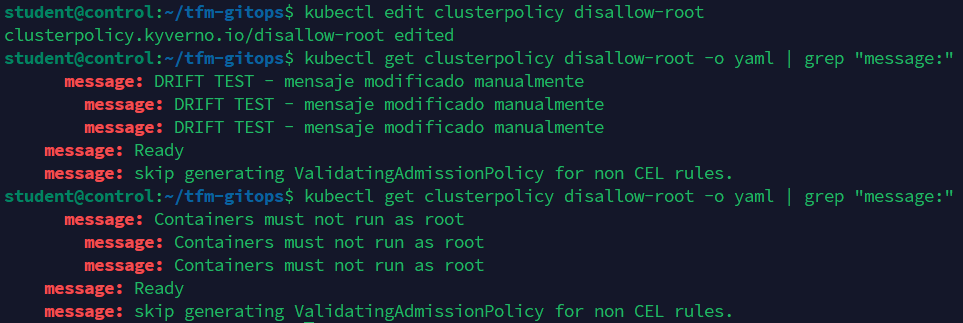
\includegraphics[width=0.95\linewidth]{actions/bloque4_prueba1ModificadoPolicy.png}
\caption{Prueba 1: modificación manual revertida por ArgoCD mediante \texttt{selfHeal}}
\label{fig:prueba1-modificacion}
\end{figure}

En este experimento, la reversión se produjo en cuestión de segundos. Aunque el intervalo de \textit{polling} del repositorio Git está configurado por defecto en 3~minutos, ArgoCD mantiene de forma paralela un \textit{watch} continuo sobre los recursos sincronizados mediante la API de Kubernetes, lo que le permite detectar cambios en el clúster casi en tiempo real e iniciar el ciclo de reconciliación de forma inmediata sin esperar al siguiente ciclo de \textit{polling} de Git.

\subsection{Despliegue de política vía commit a Git}

La segunda prueba demuestra el flujo GitOps en sentido descendente: Git como mecanismo de aprovisionamiento sin acceso directo al clúster. Se crea una nueva política, \texttt{disallow-latest-tag}, que rechaza pods cuyas imágenes estén etiquetadas con \texttt{:latest} —una práctica que impide la reproducibilidad de los despliegues al referirse a una imagen cuyo contenido puede cambiar sin aviso. La política se crea directamente en el directorio \texttt{policies/} del repositorio local, se referencia en el \texttt{kustomization.yaml} y se sube mediante commit y push al repositorio remoto.

La Figura~\ref{fig:prueba2-commit} muestra el proceso completo: creación del fichero, modificación del \texttt{kustomiza\-tion.yaml}, commit y push. El mensaje del commit, \texttt{feat: add disallow-latest-tag policy in kustomization.yaml}, documenta la intención del cambio.

\begin{figure}[H]
\centering
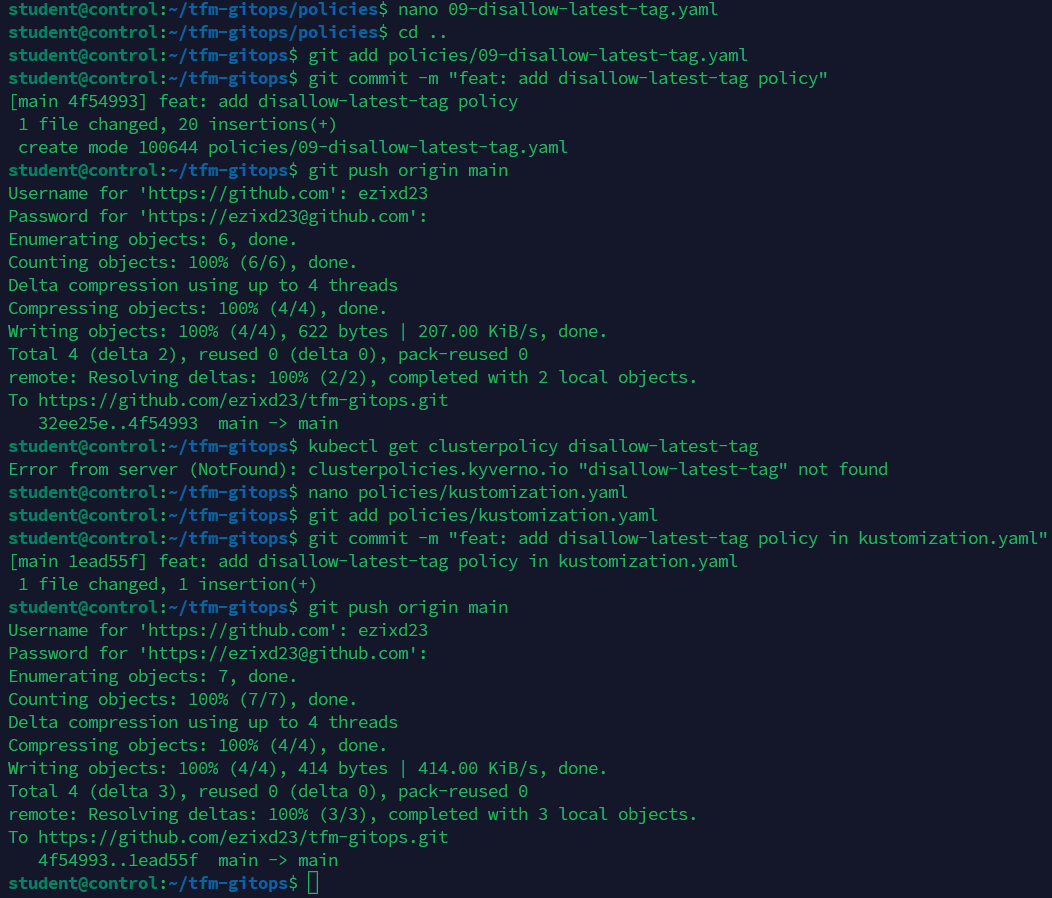
\includegraphics[width=0.95\linewidth]{actions/bloque4_prueba2CreacionyCommitNuevaPolicy.png}
\caption{Prueba 2: creación de nueva política mediante commit a Git}
\label{fig:prueba2-commit}
\end{figure}
\vspace{-\parskip}

La Figura~\ref{fig:prueba2-desplegada} confirma que la política \texttt{disallow-latest-tag} ha sido desplegada en el clúster por ArgoCD sin ninguna intervención directa, con una antigüedad de 2~minutos y 42~segundos frente a las demás políticas que llevan más de una hora activas. El campo \texttt{BACKGROUND:\,false} refleja que esta política, por su diseño basado en condiciones de exclusión, no genera evaluaciones retroactivas sobre pods existentes.

\begin{figure}[H]
\centering
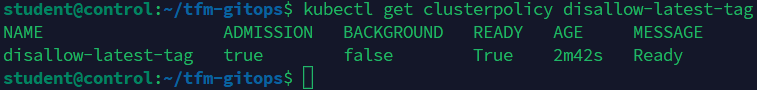
\includegraphics[width=0.90\linewidth]{actions/bloque4_prueb2PolicyDesplegada.png}
\caption{Prueba 2: \texttt{disallow-latest-tag} desplegada automáticamente por ArgoCD (2m42s de antigüedad)}
\label{fig:prueba2-desplegada}
\end{figure}
\vspace{-\parskip}

La interfaz de ArgoCD, mostrada en la Figura~\ref{fig:prueba2-ui}, refleja el árbol actualizado con nueve \texttt{ClusterPolicies} —la política nueva aparece como nodo adicional en el grafo con marca temporal de hace 2~minutos, mientras que el resto lleva sincronizado desde hace más de una hora.

\begin{figure}[H]
\centering
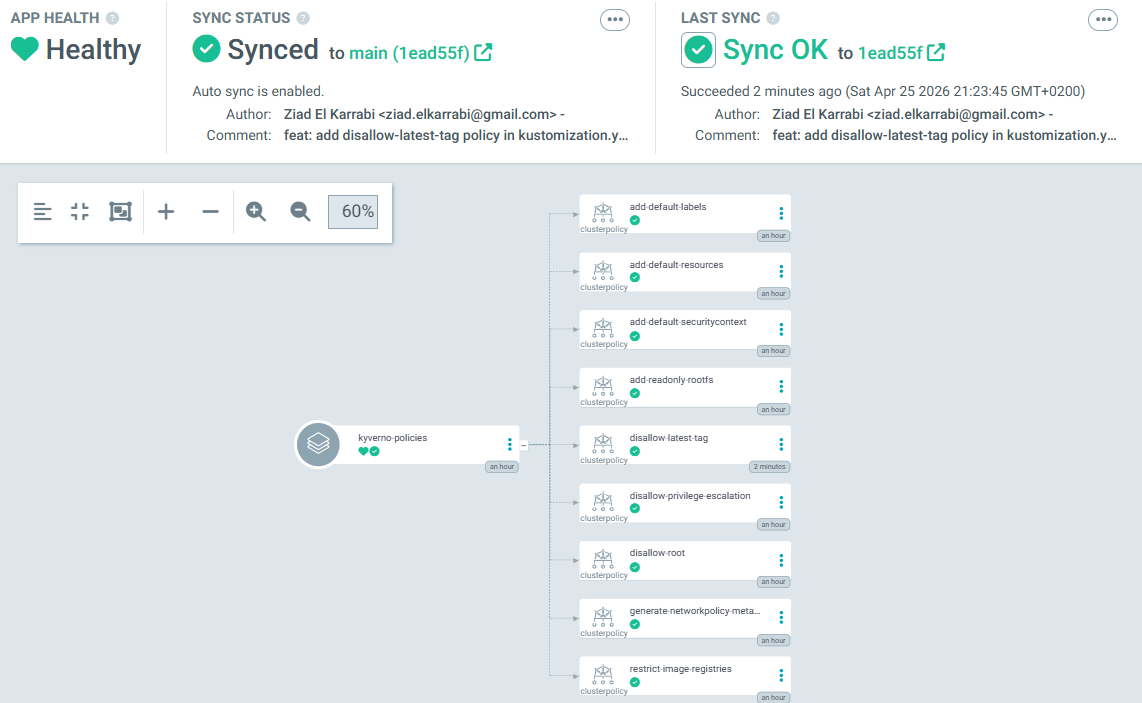
\includegraphics[width=0.95\linewidth]{actions/bloque4_prueba2AparicionUI.png}
\caption{Prueba 2: árbol de ArgoCD actualizado con la nueva política \texttt{disallow-latest-tag}}
\label{fig:prueba2-ui}
\end{figure}
\vspace{-\parskip}

\subsection{Protección ante eliminación}

La tercera prueba verifica que ArgoCD restaura automáticamente una política eliminada directamente del clúster. Este escenario complementa la prueba de \textit{drift protection} de Kyverno documentada en la Sección~6.5, donde se demostró que el Background Controller restaura la NetworkPolicy \texttt{block-cloud-metadata} generada por P8. En este caso, la eliminación afecta a la propia política fuente que la genera.

Se elimina la política \texttt{disallow-root} mediante \texttt{kubectl delete clusterpolicy\allowbreak disallow-root}. La Figura~\ref{fig:prueba3-eliminacion} muestra la secuencia: la eliminación se confirma con el mensaje \texttt{clusterpolicy.\allowbreak kyverno.\allowbreak io "disallow-root" deleted}; la consulta inmediatamente posterior devuelve un resultado vacío. Sin embargo, 48~segundos después, una nueva consulta muestra la política de nuevo en estado \texttt{Ready}, con una antigüedad de 48~segundos frente a los minutos de las demás, confirmando que ArgoCD la ha recreado.
\begin{figure}[H]
\centering
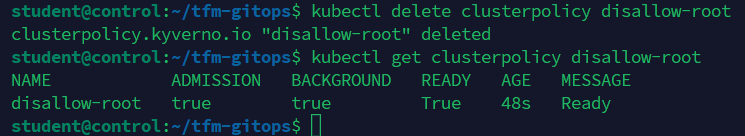
\includegraphics[width=0.90\linewidth]{actions/bloque4_prueba3ProteccionAnteEliminacion.png}
\caption{Prueba 3: política \texttt{disallow-root} restaurada por ArgoCD 48~s tras su eliminación manual}
\label{fig:prueba3-eliminacion}
\end{figure}

La combinación de las tres pruebas demuestra que el sistema opera con dos capas de protección ortogonales: ArgoCD garantiza que las políticas definidas en Git siempre existen y no son modificadas; Kyverno garantiza que los recursos generados por esas políticas (NetworkPolicies) tampoco pueden ser eliminados ni modificados. La eliminación de cualquier capa de protección no compromete la seguridad completa del sistema, pero sí reduce su superficie de resiliencia.

% ─────────────────────────────────────────────
\section{Application para la aplicación demo}
% ─────────────────────────────────────────────

La arquitectura GitOps implementada hasta este punto gestiona únicamente el plano de políticas de plataforma. Para completar la arquitectura de dos planos descrita en la Sección~5.1 y demostrar que el sistema funciona de forma integrada para cargas de trabajo reales, se implementa una segunda \texttt{Application} que despliega una aplicación demo gestionada declarativamente desde el mismo repositorio GitOps.

\subsection{Diseño de la aplicación demo}

La imagen base elegida es \texttt{nginxinc/nginx-unprivileged:1.27-alpine}, disponible en \texttt{docker.io} bajo el prefijo \texttt{nginxinc/} que satisface la política P3 (\texttt{restrict-image-regist\-ries}). La variante \textit{unprivileged} de la imagen nginx oficial está diseñada específicamente para ejecutarse sin privilegios de root: el proceso nginx escucha en el puerto~8080 en lugar del puerto~80 (que requeriría \texttt{CAP\_NET\_BIND\_SERVICE}) y ejecuta con el UID~101, siendo compatible con la política P1 (\texttt{disallow-root}) sin necesidad de configuración adicional.

Los manifiestos de la aplicación demo son tres:

\textbf{Namespace} (\texttt{namespace.yaml}): declara el namespace \texttt{demo-app} con labels de identificación. El label \texttt{purpose:\,tfm-demo} es relevante porque su existencia activa la política P8 (\texttt{generate-networkpolicy-metadata}), que generará automáticamente la NetworkPolicy de bloqueo del IMDS en cuanto el namespace sea creado.

\textbf{Deployment} (\texttt{deployment.yaml}), cuyo contenido se muestra en la Figura~\ref{fig:demo-deployment}: especifica 2~réplicas de la imagen \texttt{nginx-unprivileged}, el \texttt{securityContext} a nivel de pod con \texttt{runAsNonRoot:\,true} y \texttt{runAsUser:\,101}, y tres montajes de volumen de tipo \texttt{emptyDir} —\texttt{/tmp}, \texttt{/var/cache/nginx} y \texttt{/var/run}. La inclusión de estos tres volúmenes responde directamente a la política P6 (\texttt{add-readonly-rootfs}), que fuerza el sistema de ficheros raíz a modo de solo lectura: nginx requiere escribir ficheros PID en \texttt{/var/run}, archivos de caché en \texttt{/var/cache/nginx} y ficheros temporales en \texttt{/tmp}, y sin los volúmenes correspondientes el proceso fallaría al iniciarse. Esta configuración materializa la lección documentada en la Sección~6.4.3: la política no se debilita, sino que obliga al desarrollador a ser explícito sobre las necesidades de escritura de su aplicación.

\begin{figure}[H]
\centering
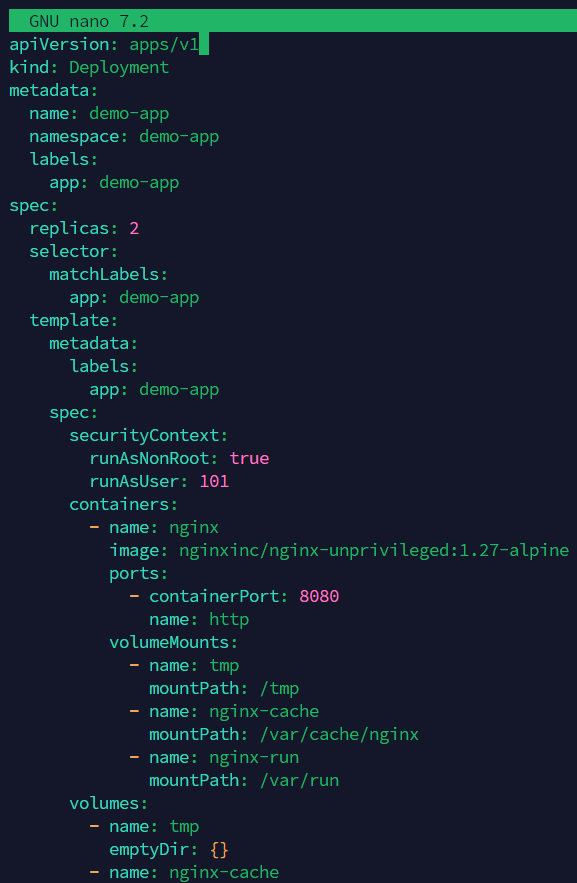
\includegraphics[width=0.70\linewidth]{actions/bloque5_deploymnet.png}
\caption{Manifiesto \texttt{deployment.yaml} de la aplicación demo con tres volúmenes \texttt{emptyDir}}
\label{fig:demo-deployment}
\end{figure}
\vspace{-\parskip}

\textbf{Service} (\texttt{service.yaml}): expone la aplicación mediante un \texttt{ClusterIP} que mapea el puerto~80 al puerto~8080 del contenedor, con un \texttt{NodePort} adicional configurado en \texttt{8888} para el acceso desde el laboratorio.

\subsection{Manifiesto de la Application y despliegue}

El manifiesto \texttt{app-demo.yaml}, mostrado en la Figura~\ref{fig:app-demo-yaml}, define la \texttt{Application} de ArgoCD para la carga de trabajo. Hay una diferencia de diseño deliberada respecto a \texttt{app-policies.yaml}: el campo \texttt{selfHeal} está configurado a \texttt{false}.

\begin{figure}[H]
\centering
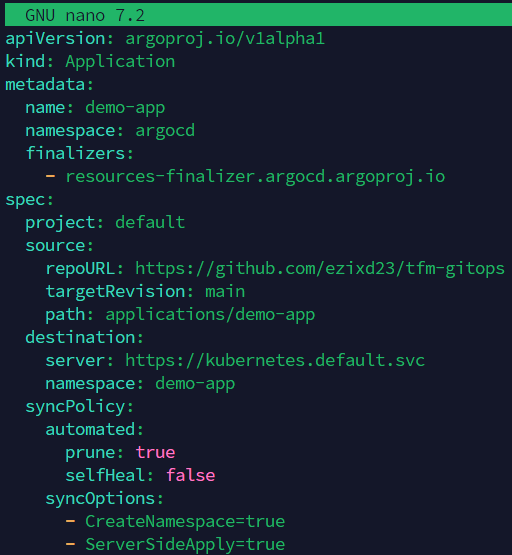
\includegraphics[width=0.70\linewidth]{actions/bloque5_app-demo.png}
\caption{Manifiesto \texttt{app-demo.yaml}: Application para la carga de trabajo con \texttt{selfHeal:\,false}}
\label{fig:app-demo-yaml}
\end{figure}

Esta decisión refleja una distinción operativa importante entre los dos planos gestionados. Las políticas de seguridad son activos de plataforma cuya integridad es crítica: cualquier desviación de su estado declarativo en Git constituye una potencial degradación de la postura de seguridad y debe ser revertida automáticamente. Los recursos de una carga de trabajo, en cambio, pueden ser modificados temporalmente por el equipo de operaciones para diagnóstico, por scripts de escalado automático o por otros controladores del clúster sin que esto represente un problema de seguridad. El \texttt{selfHeal:\,false} delega en el equipo la decisión de cuándo reconciliar, manteniendo el control declarativo (Git como fuente de verdad) pero sin la reversión automática que puede interferir con operaciones legítimas.

Tras aplicar el manifiesto, ArgoCD detecta la divergencia entre el repositorio y el clúster (que aún no contiene ningún recurso del namespace \texttt{demo-app}) y procede a la sincronización. La Figura~\ref{fig:demo-argocd} muestra el árbol de recursos resultante: la \texttt{Application} \texttt{demo-app} gestiona el Namespace, el Service y el Deployment, que a su vez genera un ReplicaSet con dos Pods activos.

\begin{figure}[H]
\centering
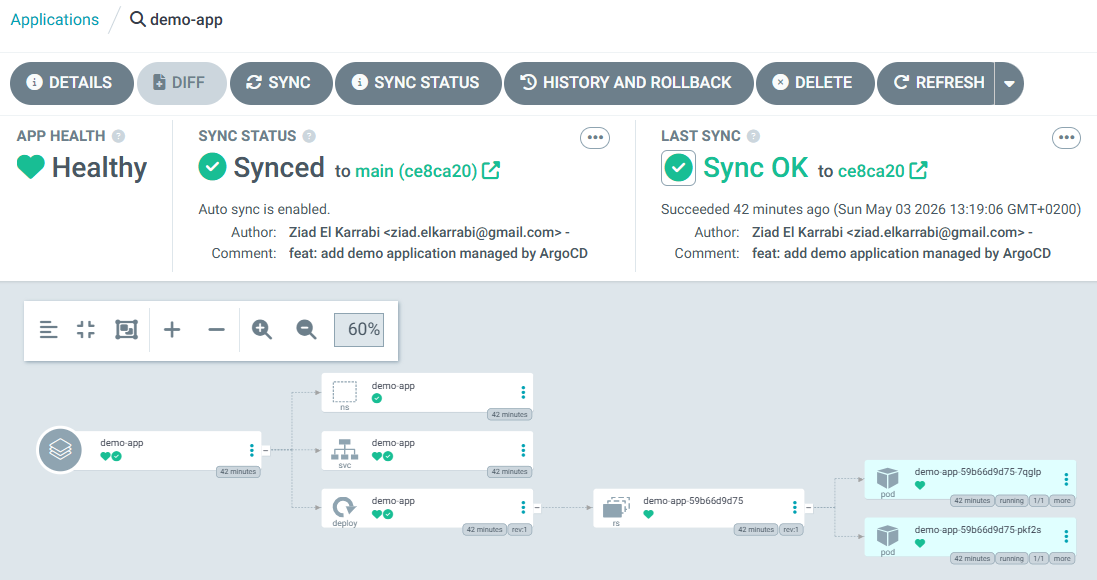
\includegraphics[width=0.95\linewidth]{actions/bloque5_argocd-demo-app.png}
\caption{Árbol de recursos de la Application \texttt{demo-app}: Namespace, Service, Deployment y dos Pods}
\label{fig:demo-argocd}
\end{figure}

\subsection{Verificación de las mutaciones de Kyverno}

La Figura~\ref{fig:demo-outputs} muestra la verificación integrada de los efectos de las políticas de mutación sobre los pods de la aplicación demo.

\begin{figure}[H]
\centering
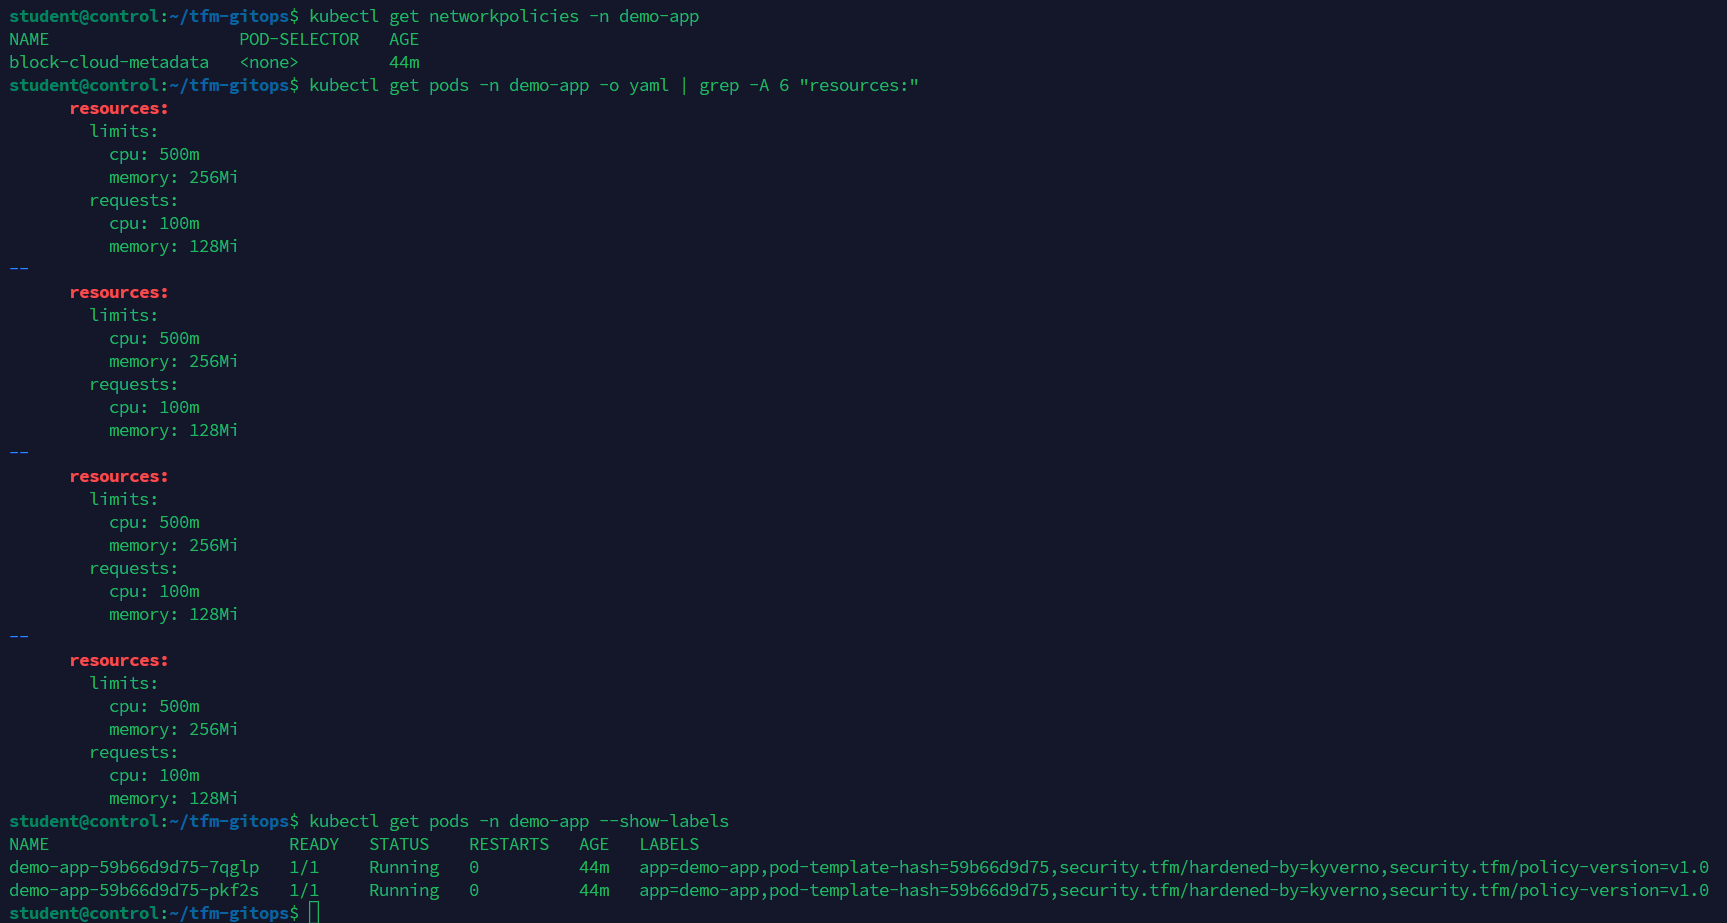
\includegraphics[width=0.95\linewidth]{actions/bloque5_ouputsP4P7P8.png}
\caption{Verificación de las mutaciones P4, P7 y P8 sobre los pods de la aplicación demo}
\label{fig:demo-outputs}
\end{figure}

La consulta \texttt{kubectl get networkpolicies -n demo-app} confirma que la NetworkPolicy \texttt{block-cloud-metadata} ha sido generada automáticamente por P8 en el namespace \texttt{demo-app} en el momento de su creación, sin ninguna intervención manual. La NetworkPolicy existe desde hace 44~minutos, periodo idéntico al del resto de recursos del namespace, lo que confirma que la generación se produjo de forma inmediata.

La consulta del siguiente comando:

\begin{lstlisting}
kubectl get pods -n demo-app -o yaml | grep -A 6 "resources:"
\end{lstlisting}

muestra que todos los contenedores de los pods del ReplicaSet tienen inyectados los campos \texttt{limits} (cpu:\,500m, memory:\,256Mi) y \texttt{requests} (cpu:\,100m, memory:\,128Mi) por la política P4, pese a que el Deployment declarado en Git no especifica ningún campo \texttt{resources}. El recuento de cuatro bloques de \texttt{resources} se debe a que el comando \texttt{grep} captura todas las ocurrencias del patrón \texttt{resources:} en el manifiesto YAML del pod ---tanto en \texttt{spec.containers} (la especificación deseada) como en \texttt{status.containerStatuses} (el estado real reportado por el kubelet)---, repetido para los dos pods activos del ReplicaSet.

La consulta \texttt{kubectl get pods -n demo-app -{}-show-labels} confirma la presencia de los labels \texttt{security.tfm/\allowbreak hardened-by:\,\allowbreak kyverno} y \texttt{security.tfm/\allowbreak policy-version:\,\allowbreak v1.0} inyectados por P7 en ambos pods, junto a los labels propios del Deployment (\texttt{app:\,\allowbreak demo-app}, \texttt{pod-template-hash}).
La verificación HTTP, mostrada en la Figura~\ref{fig:nginx-ok}, confirma que la aplicación es funcionalmente correcta pese al conjunto completo de restricciones de seguridad aplicadas: nginx responde correctamente en \texttt{192.168.1.101:8888}.

\begin{figure}[H]
\centering
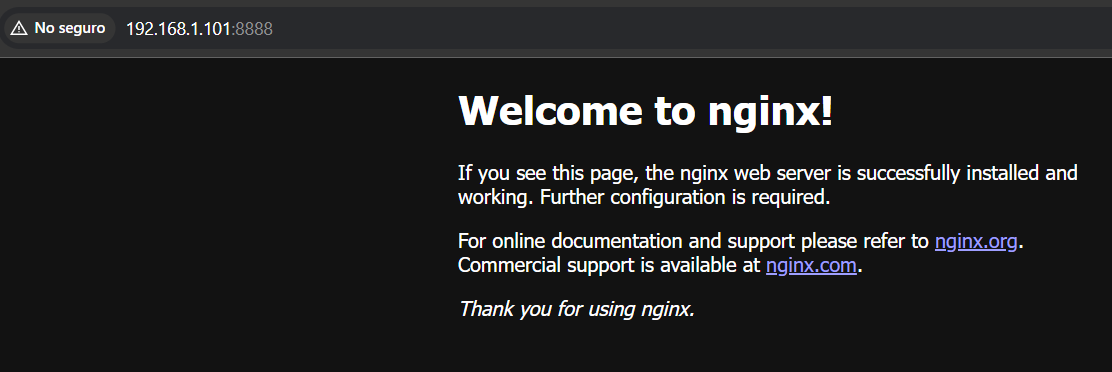
\includegraphics[width=0.85\linewidth]{actions/bloque5_outputNgnixFuncionando.png}
\caption{Aplicación demo accesible y funcional en \texttt{192.168.1.101:8888} con todas las políticas activas}
\label{fig:nginx-ok}
\end{figure}

La Figura~\ref{fig:dos-applications} muestra el estado final del panel de ArgoCD con las dos \texttt{Application} —\texttt{demo-app} y \texttt{kyverno-policies}— ambas en estado \texttt{Healthy}~+~\texttt{Synced}, materializando la arquitectura de doble plano GitOps descrita en el Capítulo~5.

\begin{figure}[H]
\centering
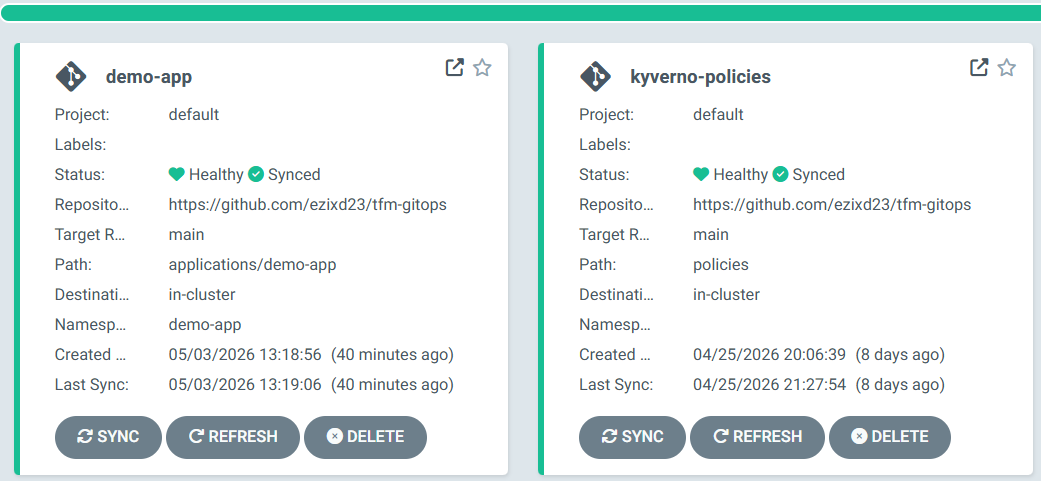
\includegraphics[width=0.85\linewidth]{actions/bloque5_dosAplications.png}
\caption{Estado final del panel de ArgoCD: dos Applications en estado Healthy y Synced}
\label{fig:dos-applications}
\end{figure}

% ─────────────────────────────────────────────
\section{Análisis: interacción entre mutating webhooks y ArgoCD}
\label{sec:argocd-mutating}
% ─────────────────────────────────────────────

La documentación oficial de ArgoCD advierte de forma explícita que la presencia de \textit{mutating admission controllers} en el clúster puede generar \textit{drift} permanente \cite{argocd_diffing}: si un webhook modifica un recurso después de que ArgoCD lo haya sincronizado, el estado en el clúster diferirá del estado en Git de forma indefinida, manteniendo la \texttt{Application} en estado \texttt{OutOfSync} de forma crónica. La solución prescrita son las opciones \texttt{ignoreDifferences} o \texttt{ServerSideApply}. La sección~\ref{sec:ignore-differences} ya documentó la aplicación de esta solución para el caso de los defaults inyectados por Kyverno sobre las propias \texttt{ClusterPolicies}. Este apartado analiza si el mismo problema se manifiesta para las mutaciones que Kyverno aplica sobre los pods de la aplicación demo.

\subsection{Comportamiento observado: ausencia de drift en la Application demo}

La \texttt{Application} \texttt{demo-app} se mantiene en estado \texttt{Synced}~+~\texttt{Healthy} de forma estable, como confirma la Figura~\ref{fig:escenario1-sync}, pese a que sus pods son mutados por las cuatro políticas P4--P7. Este resultado, que podría parecer contraintuitivo dada la advertencia de la documentación, tiene una explicación técnica precisa.

\begin{figure}[H]
\centering
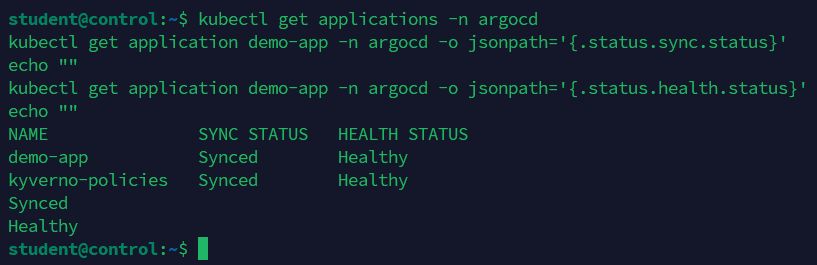
\includegraphics[width=0.85\linewidth]{actions/bloque5_escenario1Sync.png}
\caption{Ambas Applications en estado Synced y Healthy: la mutación de pods no genera drift en ArgoCD}
\label{fig:escenario1-sync}
\end{figure}

ArgoCD compara los recursos al mismo nivel jerárquico en el que están declarados en Git. El repositorio contiene un recurso de tipo \texttt{Deployment}, no recursos de tipo \texttt{Pod} directamente. Las mutaciones de Kyverno —P4 (resources), P5 (securityContext), P6 (readOnlyRootFilesystem) y P7 (labels)— se aplican sobre los \texttt{Pod} en el momento de su creación por el ReplicaSet, no sobre el campo \texttt{spec.template} del \texttt{Deployment}. ArgoCD compara el \texttt{Deployment} declarado en Git con el \texttt{Deployment} existente en el clúster, y estos coinciden. Los \texttt{Pod} generados como recursos hijos no son gestionados directamente por ArgoCD y no forman parte de la comparación.

La verificación empírica de este comportamiento, documentada en la Figura~\ref{fig:escenario1-mutacion}, compara el contenido del \texttt{Deployment} y de un \texttt{Pod} en el clúster mediante búsqueda de los campos relevantes:

\begin{figure}[H]
\centering
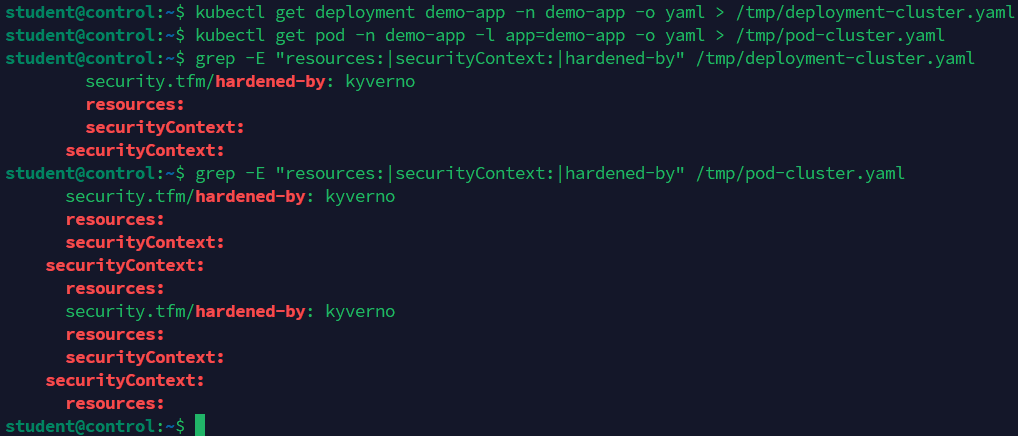
\includegraphics[width=0.95\linewidth]{actions/bloque5_escenario1Mutacion.png}
\caption{Comparativa Deployment vs. Pod: las mutaciones existen en el Pod pero no en el \texttt{spec.template} del Deployment}
\label{fig:escenario1-mutacion}
\end{figure}

La búsqueda sobre \texttt{/tmp/deployment-cluster.yaml} devuelve \texttt{resources:} con valor vacío (el campo existe en el objeto pero sin valores asignados en el template) y \texttt{securityContext:} únicamente con \texttt{runAsNonRoot:\,true} y \texttt{runAsUser:\,101}, que corresponden a los valores declarados explícitamente en el manifiesto Git. La búsqueda sobre \texttt{/tmp/pod-cluster.yaml} devuelve \texttt{resources:} con los valores inyectados por P4 (\texttt{limits} y \texttt{requests}), múltiples entradas de \texttt{securityContext:} con los valores inyectados por P5 y P6, y la presencia del label \texttt{security.tfm/hardened-by:\,kyverno} inyectado por P7. Los campos inyectados existen en el Pod pero no en el Deployment, y ArgoCD solo compara Deployments.

Esta observación está relacionada con el mecanismo de autogen descrito en la Sección~\ref{subsec:autogen}. Las reglas \texttt{autogen-add-resources}, \texttt{autogen-add-default-securitycontext} y similares, visibles en la Figura~\ref{fig:autogen-deployment}, generan reglas adicionales que se aplican sobre el \texttt{spec.template.spec} de los controllers superiores, no únicamente sobre los Pods resultantes.

\begin{figure}[H]
\centering
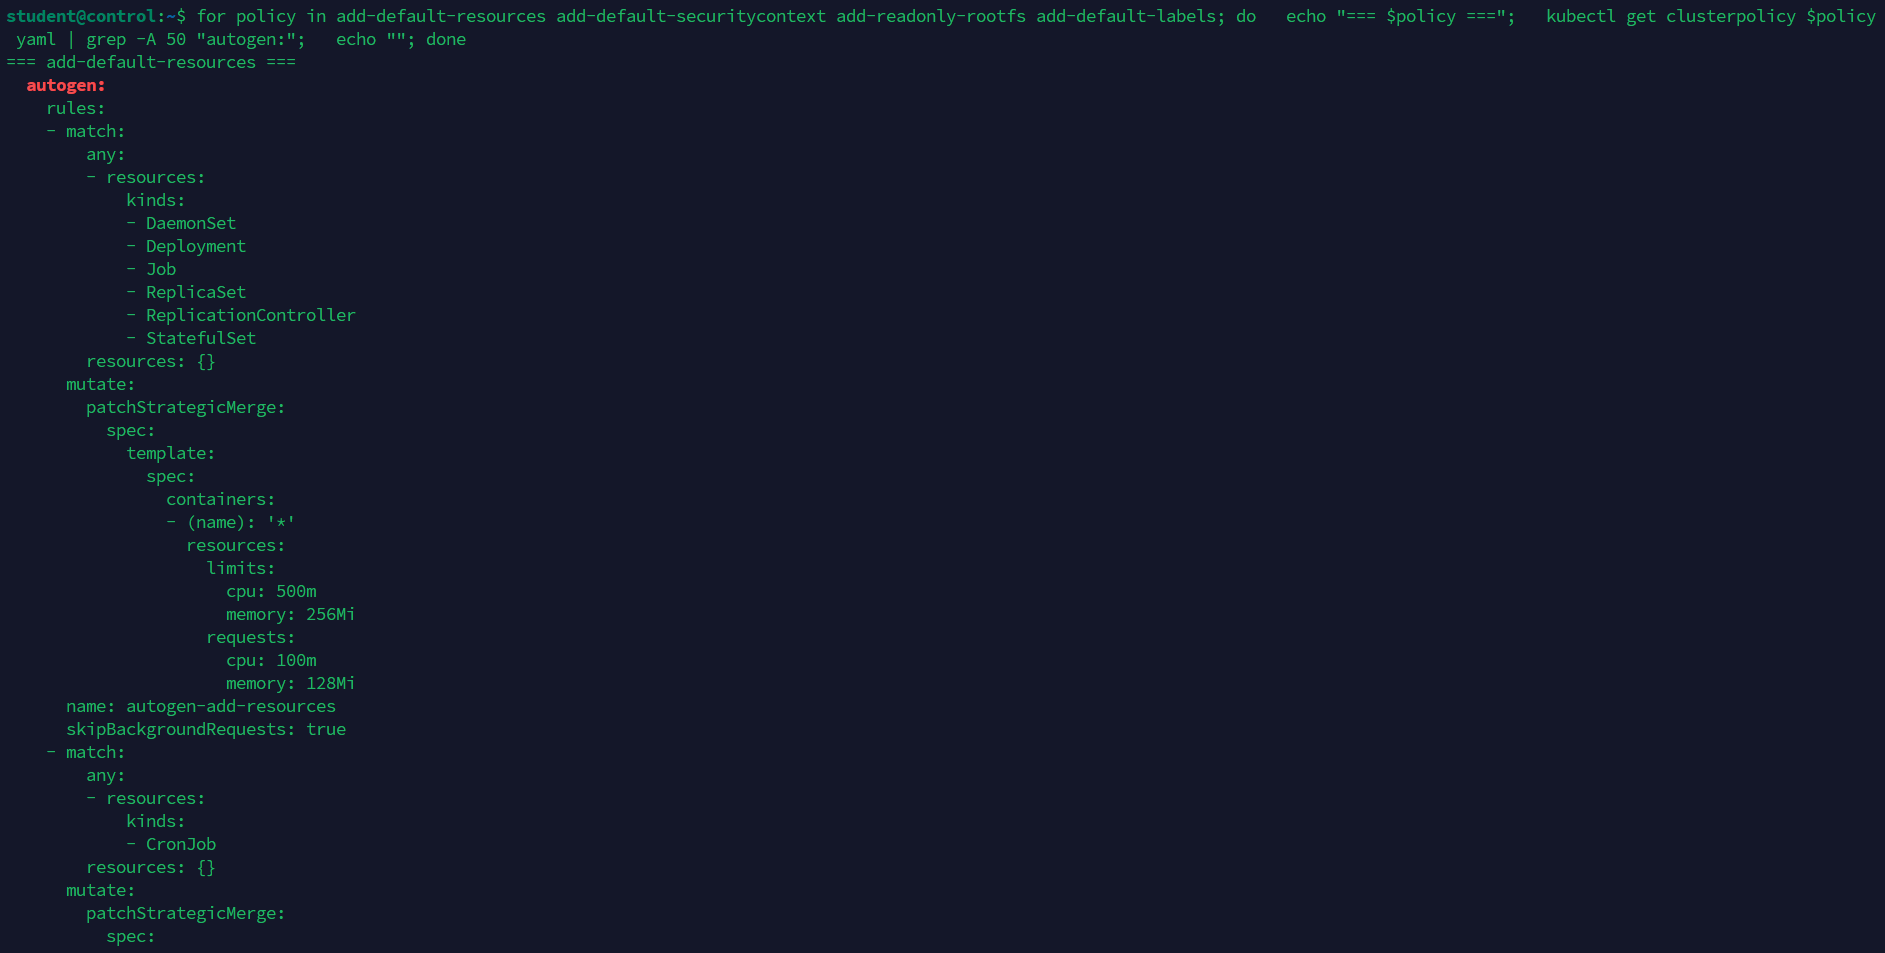
\includegraphics[width=0.95\linewidth]{actions/bloque5_escenario1Autogen.png}
\caption{Reglas autogen de la política P4: cubren Deployment, StatefulSet, Job, ReplicaSet vía \texttt{spec.template.spec}}
\label{fig:autogen-deployment}
\end{figure}

Sin embargo, la comparación empírica demuestra que el \texttt{spec.template} del Deployment en el clúster no contiene los campos inyectados. Esto indica que en la versión de Kyverno utilizada (v1.13) con \texttt{patchStrategicMerge}, la mutación efectiva se produce únicamente sobre el objeto \texttt{Pod} en el momento de su creación por el ReplicaSet, no sobre el \texttt{spec.template} del Deployment en el momento de su admisión. Este comportamiento es consistente con el principio de mínima interferencia con sistemas declarativos externos como ArgoCD.

\subsection{Verificación del caso en que sí se produce drift}

Para confirmar que el mecanismo descrito es correcto y no simplemente una ausencia de mutación, se diseña una política experimental —\texttt{experimental-\allowbreak deployment-\allowbreak labels}— que muta explícitamente recursos de tipo \texttt{Deployment} añadiendo un label \texttt{experimental.tfm/\allowbreak deployment-mutated:\,\allowbreak "true"} directamente sobre el objeto \texttt{Deployment}, como muestra la Figura~\ref{fig:policy-experimental}.
\begin{figure}[H]
\centering
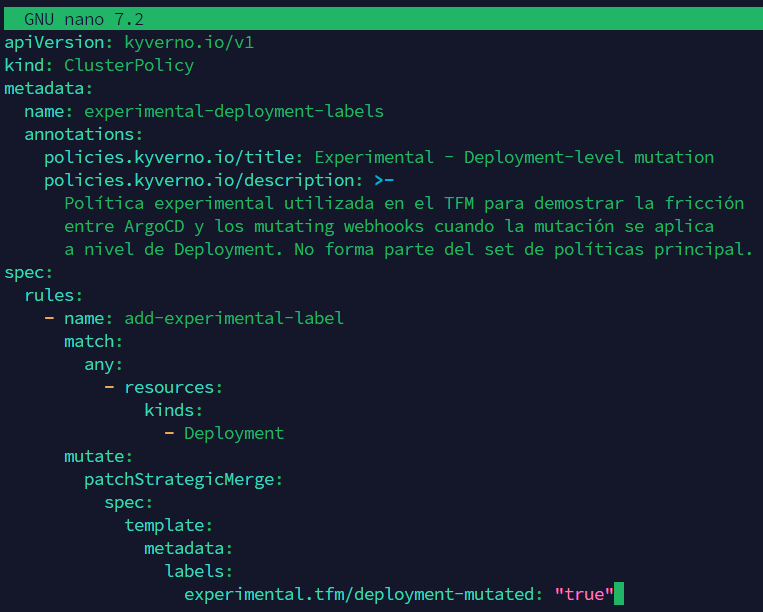
\includegraphics[width=0.72\linewidth]{actions/bloque5_escenario2policy-experimental-deployment-labels.png}
\caption{Política experimental que muta directamente recursos de tipo \texttt{Deployment}}
\label{fig:policy-experimental}
\end{figure}
\vspace{-\parskip}

La Figura~\ref{fig:escenario2-outsync} muestra el resultado: inmediatamente tras aplicar esta política en el clúster, la \texttt{Application} \texttt{demo-app} pasa a estado \texttt{OutOfSync} mientras que \texttt{kyverno-policies} permanece \texttt{Synced}. El \texttt{Deployment} en el clúster ahora tiene el label adicional que no está declarado en Git, y ArgoCD detecta la divergencia de forma correcta.

\begin{figure}[H]
\centering
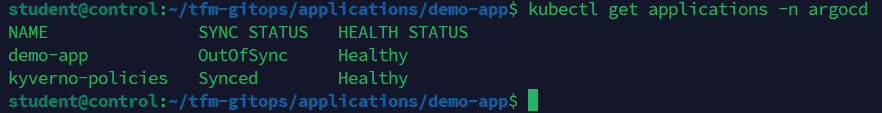
\includegraphics[width=0.85\linewidth]{actions/bloque5_escenario2OutputdelComandoKubectl.png}
\caption{Prueba del caso de drift real: \texttt{demo-app} pasa a OutOfSync al mutar directamente el Deployment}
\label{fig:escenario2-outsync}
\end{figure}

Este experimento confirma dos cosas simultáneamente: primero, que el mecanismo de detección de drift de ArgoCD funciona correctamente cuando la mutación afecta al nivel del recurso gestionado; segundo, que las políticas de mutación del conjunto principal (P4--P7) no generan este efecto porque operan a nivel Pod y no a nivel Deployment, lo que constituye el diseño correcto para su coexistencia con sistemas GitOps.

\subsection{Conclusión y patrón de resolución}

El análisis empírico permite formular una conclusión técnica precisa: en el setup implementado, la fricción entre los \textit{mutating webhooks} de Kyverno y ArgoCD no se manifiesta para las políticas de mutación del conjunto principal porque estas operan sobre un nivel jerárquico distinto al de los recursos gestionados por ArgoCD. La advertencia de la documentación oficial es correcta en general, pero no aplicable en este diseño específico.

En escenarios donde las políticas mutaran directamente recursos del mismo tipo que los gestionados en Git —por ejemplo, mutaciones de \texttt{spec.replicas} en Deployments o adición de labels a nivel de Deployment— sería necesario configurar \texttt{ignoreDifferences} en la \texttt{Application} correspondiente para los campos afectados. El patrón de resolución ya documentado en la Sección~\ref{sec:ignore-differences} —uso de \texttt{jqPathExpressions} para excluir los campos modificados por el sistema— es directamente aplicable a este caso, sin requerir cambios en los manifiestos de Git ni en las políticas de Kyverno.

\chapter{Integración Continua con GitHub Actions y análisis de vulnerabilidades}

El presente capítulo documenta la implementación del plano de Integración Continua del entorno DevSecOps, completando la arquitectura diseñada en el Capítulo~5 y cerrando el ciclo CI/CD iniciado con ArgoCD en el Capítulo~7. Hasta este punto, la arquitectura GitOps operaba con un único repositorio (\texttt{tfm-gitops}) que combinaba manifiestos de Kubernetes y políticas de seguridad, gestionado declarativamente por ArgoCD. El presente capítulo materializa el \textit{patrón de dos repositorios} anunciado en la Sección~7.1: se introduce un segundo repositorio (\texttt{tfm-demo-app}) que contiene el código fuente de la aplicación y su Dockerfile, y se implementa el pipeline de Integración Continua que construye la imagen, la somete a análisis de seguridad y propaga el cambio al repositorio GitOps para su despliegue automático.

Una característica técnica central del pipeline es la adopción de una estrategia de \textit{defensa en profundidad} en el análisis de vulnerabilidades: en lugar de un único motor de escaneo, se implementan dos motores complementarios. Trivy \cite{trivy_docs} analiza la imagen construida localmente, y Grype \cite{grype_docs} analiza un SBOM (\textit{Software Bill of Materials}) \cite{syft_docs} generado por Syft sobre esa misma imagen, consultando bases de datos de CVEs distintas. El hallazgo empírico que justifica esta estrategia ---Trivy dejó pasar la imagen \texttt{python:3.12-slim} sin alertas mientras Grype detectó una vulnerabilidad HIGH que bloqueó el pipeline--- constituye uno de los resultados más relevantes del trabajo.

El capítulo se organiza en siete secciones. La primera justifica la separación en dos repositorios y documenta su estructura. La segunda describe la configuración del registro de imágenes y las credenciales del pipeline. La tercera documenta la aplicación de demostración y sus Dockerfiles. La cuarta describe el diseño del workflow de GitHub Actions y sus decisiones de seguridad. La quinta analiza en profundidad la estrategia de doble motor de escaneo y el hallazgo empírico clave. La sexta recoge las incidencias técnicas y las lecciones aprendidas durante la implementación. La séptima documenta el cierre del ciclo CI/CD completo y la integración con el repositorio GitOps.

% ─────────────────────────────────────────────
\section{Diseño del repositorio de aplicación y estrategia de dos repositorios}
% ─────────────────────────────────────────────

La separación entre el repositorio de aplicación y el repositorio de configuración no responde a una preferencia organizativa, sino a un requisito de seguridad concreto justificado en la Sección~5.5.1. El principio central es la segregación de credenciales: el pipeline de CI necesita acceso al registro de imágenes (\texttt{quay.io}) y capacidad de escritura en el repositorio de configuración, pero en ningún caso debe tener acceso directo al clúster Kubernetes. ArgoCD, a su vez, necesita acceso al repositorio de configuración para sincronizar el estado del clúster, pero no tiene razón alguna para acceder al código fuente de la aplicación. Esta separación establece un perímetro de seguridad entre las dos fases del ciclo CI/CD, de modo que el compromiso de una de ellas no implica automáticamente el compromiso de la otra.

El repositorio \texttt{tfm-demo-app} contiene exclusivamente los artefactos del plano de aplicación:

\begin{itemize}
  \item \texttt{app/}: código fuente de la aplicación Python Flask, incluyendo el módulo principal (\texttt{app.py}) y el fichero de dependencias (\texttt{requirements.txt}).
  \item \texttt{docker/}: los dos Dockerfiles del proyecto (\texttt{Dockerfile} y \texttt{Dockerfilevulnerable}).
  \item \texttt{.github/workflows/}: el workflow de GitHub Actions (\texttt{build-and-push.yaml}) que implementa el pipeline completo de CI.
\end{itemize}

El repositorio \texttt{tfm-gitops}, gestionado por ArgoCD desde el Capítulo~7, no es modificado por el equipo de desarrollo: únicamente el pipeline de CI lo actualiza, y únicamente en el campo \texttt{image} del manifiesto de la aplicación demo. Esta delimitación garantiza que los manifiestos de las políticas de seguridad (directorio \texttt{policies/}) y la configuración de las \texttt{Application} de ArgoCD permanecen bajo control estricto y separado del ciclo de desarrollo de la aplicación.

Esta arquitectura materializa el flujo descrito en la Sección~5.3.1: el commit en el repositorio de aplicación dispara el pipeline de CI, que culmina con un commit en el repositorio de configuración, que a su vez actúa como señal de disparo para ArgoCD. El clúster nunca recibe instrucciones directas del pipeline: toda la interacción con Kubernetes está mediada por el repositorio GitOps y el controlador de reconciliación.

% ─────────────────────────────────────────────
\section{Configuración del registro de imágenes y credenciales}
% ─────────────────────────────────────────────

El registro de imágenes elegido es Quay.io \cite{quay_docs}, en coherencia con las herramientas presentadas en la asignatura y como alternativa de nivel empresarial a Docker Hub. La autenticación del pipeline contra el registro se realiza mediante un \textbf{Robot Account}, un concepto central en la gestión de credenciales para sistemas de CI/CD que merece una justificación técnica explícita.

Un Robot Account es una cuenta de servicio no personal cuyas credenciales están desvinculadas de cualquier usuario individual. En un pipeline CI/CD, el uso de credenciales personales presenta dos problemas de seguridad: el primero es el \textit{blast radius} en caso de compromiso ---las credenciales personales tienen acceso a todos los repositorios del usuario---; el segundo es la continuidad operativa ---si el usuario abandona la organización, el pipeline deja de funcionar---. Un Robot Account aborda ambos problemas: tiene acceso exclusivamente a los repositorios que se le asignan explícitamente, con el nivel de permiso mínimo necesario para su función.

El Robot Account creado se denomina \texttt{zelkarrabi+tfm\_ci\_robot}. La Figura~\ref{fig:ci-robotaccount} muestra su configuración de permisos en Quay.io: tiene permiso \textit{Write} (escritura) sobre el repositorio \texttt{tfm-demo-app} y permiso \textit{None} (sin acceso) sobre el repositorio \texttt{prova}, que es un repositorio de prueba no relacionado con el proyecto. Esta granularidad confirma la aplicación del principio de mínimo privilegio: el Robot Account solo puede publicar imágenes en el repositorio específico para el que ha sido creado, y no puede modificar su configuración ni acceder a otros repositorios.

\begin{figure}[H]
\centering
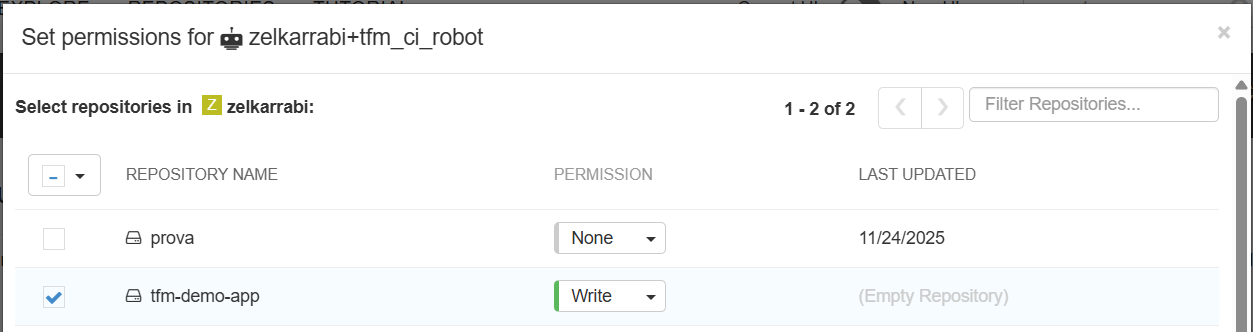
\includegraphics[width=0.90\linewidth]{ci_cd/bloque1_robotaccount.png}
\caption{Configuración del Robot Account \texttt{zelkarrabi+tfm\_ci\_robot} en Quay.io: permiso \textit{Write} sobre \texttt{tfm-demo-app} y sin acceso sobre otros repositorios}
\label{fig:ci-robotaccount}
\end{figure}

La validación de las credenciales del Robot Account se realiza previamente mediante \texttt{podman login quay.io} desde el nodo de control del clúster, lo que confirma que las credenciales son funcionales antes de configurarlas en el pipeline. La Figura~\ref{fig:ci-podmanlogin} muestra la autenticación exitosa con el usuario \texttt{zelkarrabi}.

\begin{figure}[H]
\centering
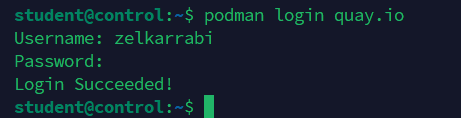
\includegraphics[width=0.60\linewidth]{ci_cd/bloque1_podmanLogin.png}
\caption{Verificación de credenciales del registro: autenticación exitosa en \texttt{quay.io} mediante \texttt{podman login}}
\label{fig:ci-podmanlogin}
\end{figure}
\vspace{-\parskip}

El pipeline requiere tres secretos de repositorio en GitHub, cuya configuración se muestra en la Figura~\ref{fig:ci-secrets}:

\begin{figure}[H]
\centering
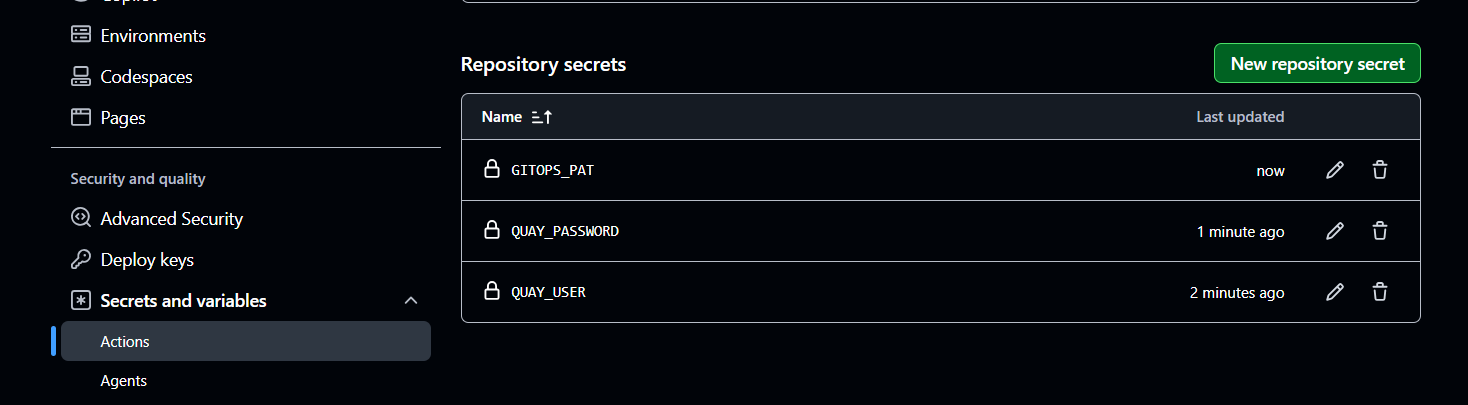
\includegraphics[width=0.90\linewidth]{ci_cd/bloque2_creaccionSecrets.png}
\caption{Los tres secretos de repositorio configurados en GitHub Actions: \texttt{GITOPS\_PAT}, \texttt{QUAY\_PASSWORD} y \texttt{QUAY\_USER}}
\label{fig:ci-secrets}
\end{figure}

\begin{itemize}
  \item \texttt{QUAY\_USER}: nombre del Robot Account (\texttt{zelkarrabi+tfm\_ci\_robot}) para la autenticación en Quay.io.
  \item \texttt{QUAY\_PASSWORD}: token de acceso generado por Quay.io para el Robot Account.
  \item \texttt{GITOPS\_PAT}: Personal Access Token de GitHub para la escritura cruzada en el repositorio \texttt{tfm-gitops}. A diferencia del Robot Account de Quay.io, un PAT clásico con scope \texttt{repo} no aplica el principio de mínimo privilegio: otorga acceso de lectura y escritura a \textit{todos} los repositorios del usuario, no solo a \texttt{tfm-gitops}. La alternativa correcta es un \textit{fine-grained PAT} limitado explícitamente a \texttt{tfm-gitops} con permiso \texttt{Contents: read/write}, que reproduce para GitHub la misma granularidad que el Robot Account ofrece en Quay.io; una \textit{deploy key} de repositorio es otra opción equivalente. En este entorno de laboratorio se utiliza un PAT clásico por simplicidad, siendo consciente de que en producción debería sustituirse por una de esas alternativas.
\end{itemize}

El uso explícito del \texttt{GITOPS\_PAT} en lugar del \texttt{GITHUB\_TOKEN} por defecto responde a una restricción técnica de GitHub Actions: el \texttt{GITHUB\_TOKEN} tiene permisos únicamente sobre el repositorio en el que se ejecuta el workflow (\texttt{tfm-demo-app}), y no puede escribir en un repositorio diferente. El \texttt{GITOPS\_PAT}, al ser un token personal con scope explícito sobre \texttt{tfm-gitops}, es el mecanismo correcto para la escritura cruzada entre repositorios.

% ─────────────────────────────────────────────
\section{La aplicación de demostración y los Dockerfiles}
% ─────────────────────────────────────────────

La aplicación de demostración es una aplicación Python Flask \cite{github_actions_docs} mínima cuya función es validar el ciclo CI/CD completo, no representar una carga de trabajo de producción real. Expone dos endpoints en el puerto~8080:

\begin{lstlisting}
from flask import Flask, jsonify
import os, socket

app = Flask(__name__)

@app.route('/')
def index():
    return jsonify({
        "service": "tfm-demo-app",
        "version": "1.0.0",
        "status": "ok",
        "hostname": socket.gethostname(),
        "ci_pipeline": os.getenv("CI_PIPELINE", "manual")
    })

@app.route('/health')
def health():
    return jsonify({"status": "healthy"})

if __name__ == '__main__':
    app.run(host='0.0.0.0', port=8080)
\end{lstlisting}

El endpoint raíz (\texttt{/}) devuelve un objeto JSON que incluye el nombre del servicio, la versión, el hostname del pod y el valor de la variable de entorno \texttt{CI\_PIPELINE}. Este último campo es el que permite verificar empíricamente, al final del capítulo, que el código desplegado en el clúster corresponde exactamente al código del commit que disparó el pipeline. El endpoint \texttt{/health} sirve de sonda de disponibilidad para los componentes de Kubernetes.

\subsection{El Dockerfile seguro: decisiones técnicas}

El Dockerfile principal incorpora varias decisiones de diseño orientadas a la seguridad que merecen justificación explícita:

\begin{lstlisting}
# Stage 1: builder
FROM python:3.13-slim AS builder
WORKDIR /build
COPY app/requirements.txt .
RUN pip install --no-cache-dir --user --upgrade pip && \
    pip install --no-cache-dir --user -r requirements.txt

# Stage 2: runtime
FROM python:3.13-slim
RUN groupadd -r -g 10001 appuser && \
    useradd -r -u 10001 -g appuser appuser

WORKDIR /app
COPY --from=builder --chown=appuser:appuser /root/.local /home/appuser/.local
COPY --chown=appuser:appuser app/app.py /app/

ENV PATH="/home/appuser/.local/bin:${PATH}" \
    PYTHONUNBUFFERED=1 \
    PYTHONDONTWRITEBYTECODE=1

USER appuser
EXPOSE 8080
CMD ["python", "/app/app.py"]
\end{lstlisting}

\textbf{Multi-stage build.} La separación entre la fase \texttt{builder} y la fase de ejecución es la decisión de mayor impacto sobre la superficie de ataque de la imagen. La fase \texttt{builder} instala las dependencias con \texttt{pip install --user}, que las deposita en \texttt{/root/.local}. La imagen de ejecución copia únicamente ese directorio ---con \texttt{--chown=appuser:appuser}--- al directorio \texttt{/home/appuser/.local} del usuario de aplicación. De este modo, el binario \texttt{pip} y sus propias dependencias transitivas no están presentes en el artefacto final, reduciendo el número de componentes escaneables y la superficie de explotación en tiempo de ejecución.

\textbf{Imagen base mínima (\texttt{python:3.13-slim}).} La variante \texttt{slim} de la imagen oficial de Python elimina los paquetes del sistema operativo no esenciales que incluye la imagen estándar. Esta elección representa un punto de equilibrio entre compatibilidad y seguridad: la imagen incluye las bibliotecas de sistema necesarias para la mayoría de aplicaciones Python, pero elimina herramientas de desarrollo, intérpretes de scripting y utilidades que podrían ser aprovechadas tras una intrusión. El extremo de esta estrategia son las imágenes \textit{distroless} \cite{distroless_docs} de Google, que eliminan incluso el shell y el gestor de paquetes, reduciendo la superficie de ataque al mínimo absoluto a costa de cierta complejidad en el diagnóstico de fallos en tiempo de ejecución.

\textbf{Usuario no root con UID~10001.} El Dockerfile crea \texttt{appuser} como cuenta de sistema (\texttt{groupadd -r}, \texttt{useradd -r}): sin shell de login, sin entrada en \texttt{/etc/passwd} con home explícito, con UID~10001 que evita colisiones con UIDs de sistema (0--999) y de usuario típicos (1000+). La instrucción \texttt{USER appuser} hace efectiva esa identidad para todos los procesos del contenedor. Esto constituye una capa de defensa en profundidad coherente con la política P1 (\texttt{disallow-root}) del capítulo~6: aunque Kyverno rechazaría cualquier pod sin \texttt{runAsNonRoot:\,true}, la defensa empieza antes, en el propio Dockerfile, de modo que la imagen opere con mínimo privilegio independientemente del clúster en que se despliegue.

\textbf{Variables de entorno de Python.} \texttt{PYTHONUNBUFFERED=1} garantiza que la salida estándar del proceso no es almacenada en buffer, lo que permite que los logs sean capturados en tiempo real por el sistema de logging de Kubernetes. \texttt{PYTHONDONTWRITEBYTECODE=1} evita la escritura de ficheros \texttt{.pyc} en el sistema de ficheros del contenedor, lo que es coherente con la política P6 (\texttt{add-readonly-rootfs}) que fuerza el sistema de ficheros raíz a modo de solo lectura: sin esta variable, Python intentaría escribir bytecode compilado y generaría errores de permisos en tiempo de ejecución.

\textbf{Flag \texttt{-{}-no-cache-dir}.} La instalación de dependencias con esta opción evita que pip almacene el caché de paquetes descargados dentro de la imagen, reduciendo su tamaño final y eliminando contenido innecesario que podría contener versiones desactualizadas de paquetes.

\subsection{El Dockerfile vulnerable como artefacto de referencia}

El repositorio incluye un segundo Dockerfile, \texttt{Dockerfilevulnerable}, basado en \texttt{python:3.4-alpine}. Python~3.4 alcanzó su fin de vida en marzo de 2019 y acumula cientos de CVEs documentadas sin corrección disponible en esa rama. Este artefacto fue diseñado originalmente como mecanismo de prueba controlada para demostrar el escenario de bloqueo del pipeline ante imágenes con vulnerabilidades críticas. Sin embargo, como se documenta en la Sección~8.6, este escenario artificial resultó innecesario: el propio ciclo de desarrollo produjo de forma orgánica un bloqueo genuino que constituye evidencia empírica de mayor valor académico que cualquier prueba artificial.

% ─────────────────────────────────────────────
\section{Diseño del pipeline de Integración Continua}
\label{sec:pipeline-design}
% ─────────────────────────────────────────────

El pipeline se define en el fichero \texttt{.github/workflows/build-and-push.yaml}. El nombre del workflow es \textit{Build, Scan and Push to Quay} y su job único se denomina \textit{Build, Trivy scan and push}. El disparador es \texttt{push} sobre la rama \texttt{main} con filtros de path que limitan la ejecución a commits que afectan al directorio \texttt{app/}, al directorio \texttt{docker/} o al propio fichero de workflow:

\begin{lstlisting}
on:
  push:
    branches: [main]
    paths:
      - 'app/**'
      - 'docker/**'
      - '.github/workflows/**'
\end{lstlisting}

Esta configuración evita que commits que afecten únicamente a documentación o ficheros auxiliares disparen innecesariamente el pipeline, reduciendo el consumo de minutos de GitHub Actions y el ruido en el historial de ejecuciones.

\subsection{Decisiones de seguridad del pipeline}

Las cuatro decisiones de diseño de seguridad del pipeline merecen justificación técnica explícita, dado que materializan directamente los principios enunciados en el Capítulo~5.

\textbf{Anclaje de versiones mediante hash SHA.} Todas las GitHub Actions de terceros utilizadas en el pipeline se referencian mediante el hash SHA completo de su commit, en lugar de mediante etiquetas de versión semántica o etiquetas flotantes como \texttt{@v4} o \texttt{@latest}. Por ejemplo:

\begin{lstlisting}
- uses: actions/checkout@b4ffde65f46336ab88eb53be808477a3936bae11  # v4.1.1
\end{lstlisting}

Esta práctica materializa la defensa frente al vector de ataque documentado en la Sección~5.5.6: una etiqueta como \texttt{@v4} puede ser redirigida por el mantenedor de la action (o por un atacante que haya comprometido su cuenta) a un commit diferente sin que el nombre de la referencia cambie. Un hash SHA, en cambio, es inmutable: si el manifiesto del workflow referencia el SHA \texttt{b4ffde65f46\ldots}, el runner ejecutará exactamente ese commit, independientemente de lo que ocurra con las etiquetas del repositorio. La limitación de este mecanismo, que se documenta como incidencia en la Sección~8.6, es que no protege frente a dependencias transitivas del propio código de la action.

\textbf{Permisos mínimos del runner.} El bloque de permisos del job declara explícitamente solo los permisos necesarios:

\begin{lstlisting}
permissions:
  contents: read
\end{lstlisting}

El \texttt{GITHUB\_TOKEN} por defecto en GitHub Actions tiene permisos de escritura sobre el repositorio. Esta declaración explícita de \texttt{contents: read} revoca esos permisos por defecto, de modo que incluso si el entorno del runner fuera comprometido durante la ejecución, el token exfiltrado no podría modificar el repositorio de la aplicación.

\textbf{Etiqueta de imagen basada en el SHA corto del commit.} La etiqueta de la imagen publicada en Quay.io se computa a partir del SHA corto del commit que disparó el pipeline:

\begin{lstlisting}
- name: Compute image tag
  id: vars
  run: |
    SHORT_SHA=$(echo "${GITHUB_SHA}" | cut -c1-7)
    echo "SHORT_SHA=${SHORT_SHA}" >> $GITHUB_OUTPUT
    echo "FULL_IMAGE=${REGISTRY}/${IMAGE_NAME}:${SHORT_SHA}" >> $GITHUB_OUTPUT
\end{lstlisting}

Esta decisión implementa el principio de trazabilidad e inmutabilidad de la cadena de suministro: cada imagen publicada en el registro corresponde biunívocamente a un commit concreto del repositorio de aplicación, permitiendo auditar en cualquier momento qué código exacto está en ejecución en el clúster. Este diseño es además coherente con la política P9 (\texttt{disallow-latest-tag}) introducida en la Sección~7.5.2, que rechaza pods cuyas imágenes estén etiquetadas con \texttt{:latest}: el pipeline nunca produce etiquetas flotantes, solo etiquetas basadas en commit SHA.

\textbf{Separación de build y push.} La imagen se construye localmente en el runner sin ser publicada (\texttt{push: false}). El escaneo de vulnerabilidades se ejecuta sobre la imagen construida localmente. Solo si todos los controles de seguridad superan sus umbrales se ejecuta el paso de publicación. Esta secuencia es la implementación del principio de \textit{fail fast}: una imagen vulnerable nunca llega al registro, eliminando el riesgo de que ArgoCD la detecte y la despliegue antes de que el incidente sea identificado y gestionado.

\subsection{Secuencia completa de pasos del pipeline}

La Figura~\ref{fig:ci-workflow-steps-final} muestra la vista de pasos del workflow completo en su versión final, con los 15 pasos que forman el pipeline en estado de éxito:

\begin{figure}[H]
\centering
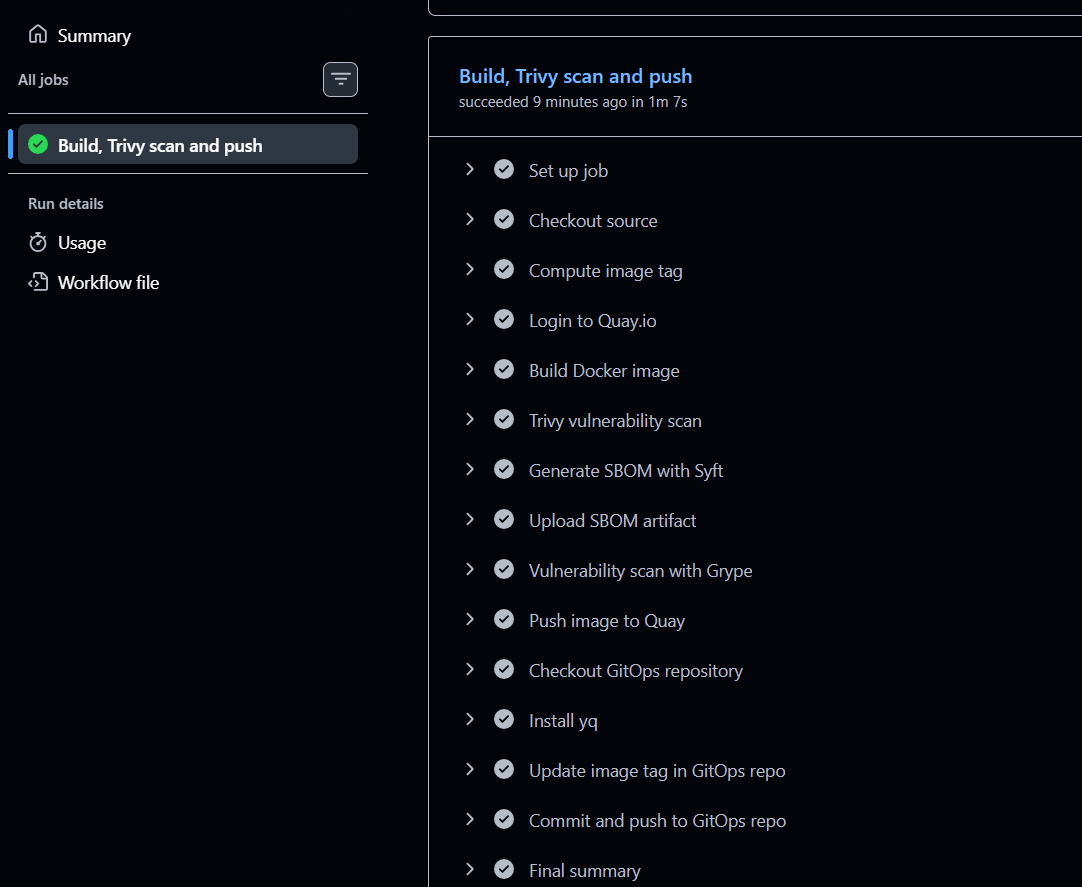
\includegraphics[width=0.70\linewidth]{ci_cd/bloque5_WorkflowCompleto.png}
\caption{Pipeline \textit{Build, Trivy scan and push} completo: los 15 pasos del ciclo CI/CD, ejecutado en 1~min~7~s}
\label{fig:ci-workflow-steps-final}
\end{figure}

La secuencia de pasos es la siguiente:

\begin{enumerate}
  \item \textbf{Set up job}: inicialización del runner \texttt{ubuntu-latest} y descarga de las actions referenciadas por SHA.
  \item \textbf{Checkout source}: clonado del repositorio \texttt{tfm-demo-app} mediante \texttt{actions/checkout} anclado por SHA.
  \item \textbf{Compute image tag}: cómputo de la etiqueta de imagen a partir de los primeros 7 caracteres del SHA del commit (\texttt{GITHUB\_SHA | cut -c1-7}), exportado como outputs \texttt{SHORT\_SHA} y \texttt{FULL\_IMAGE}.
  \item \textbf{Login to Quay.io}: autenticación en \texttt{quay.io} con las credenciales del Robot Account almacenadas en los secretos \texttt{QUAY\_USER} y \texttt{QUAY\_PASSWORD}.
  \item \textbf{Build Docker image}: construcción de la imagen mediante \texttt{docker/build-push-action} con \texttt{push:\,false}, produciendo la imagen en el daemon local del runner sin publicarla.
  \item \textbf{Trivy vulnerability scan}: escaneo de la imagen local con Trivy, configurado para fallar el pipeline ante vulnerabilidades de severidad \texttt{HIGH} o \texttt{CRITICAL} (\texttt{ignore-unfixed: true}).
  \item \textbf{Generate SBOM with Syft}: generación del Software Bill of Materials en formato CycloneDX mediante Syft \cite{syft_docs}, produciendo el fichero \texttt{sbom.cyclonedx.json}.
  \item \textbf{Upload SBOM artifact}: subida del SBOM como artefacto del workflow, accesible desde la interfaz de GitHub Actions y descargable para auditoría posterior.
  \item \textbf{Vulnerability scan with Grype}: análisis del SBOM CycloneDX con Grype \cite{grype_docs}, configurado para fallar ante vulnerabilidades de severidad \texttt{HIGH} o superior con corrección disponible (\texttt{--only-fixed}).
  \item \textbf{Push image to Quay}: publicación condicional de la imagen en el registro. Solo se ejecuta si todos los pasos de escaneo anteriores han tenido éxito.
  \item \textbf{Checkout GitOps repository}: clonado del repositorio \texttt{tfm-gitops} usando el \texttt{GITOPS\_PAT}.
  \item \textbf{Install yq}: instalación de \texttt{yq}, procesador YAML de línea de comandos.
  \item \textbf{Update image tag in GitOps repo}: actualización del campo \texttt{image} en el manifiesto \texttt{deployment.yaml} de la aplicación demo.
  \item \textbf{Commit and push to GitOps repo}: commit y push del manifiesto actualizado al repositorio GitOps.
  \item \textbf{Final summary}: resumen de la ejecución.
\end{enumerate}

La primera versión operativa del pipeline contenía únicamente los pasos 1--6 y 10 (Trivy como único motor de escaneo, sin SBOM ni Grype y sin el cierre del ciclo GitOps). La Figura~\ref{fig:ci-workflow-steps-inicial} documenta esta versión inicial, con 50~s de ejecución, que sirvió como base para validar la integración con Quay.io antes de añadir la capa de análisis SBOM.

\begin{figure}[H]
\centering
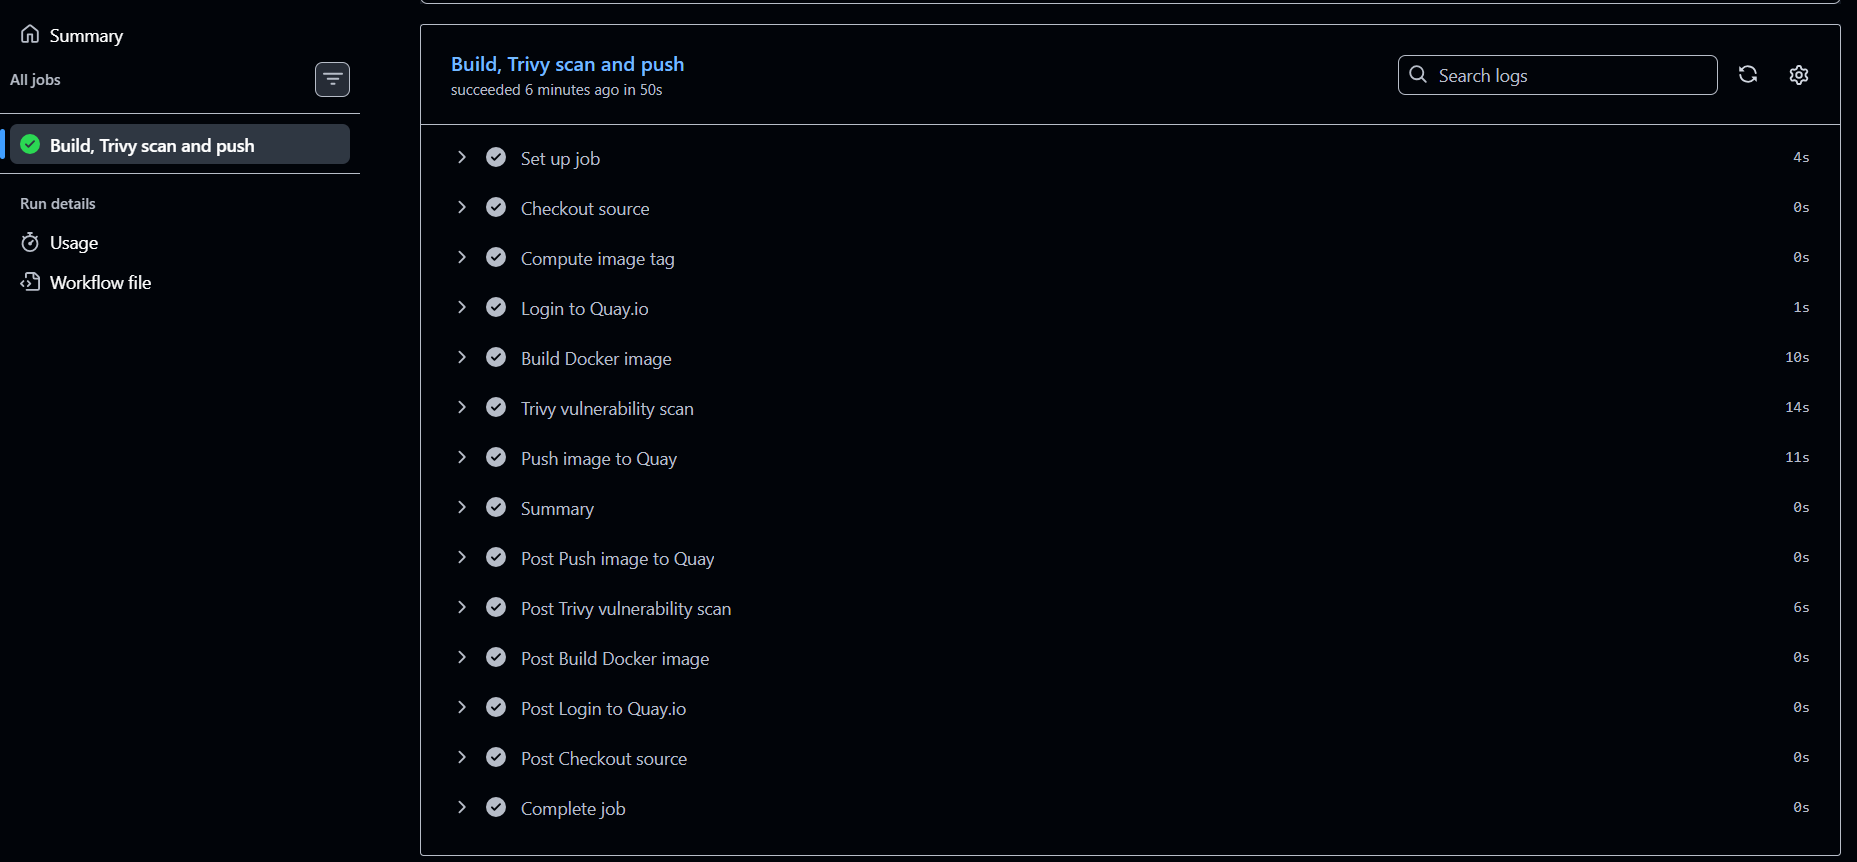
\includegraphics[width=0.90\linewidth]{ci_cd/bloque3_workflowSteps.png}
\caption{Versión inicial del pipeline \textit{Build, Trivy scan and push} (sin SBOM ni Grype): pasos de construcción, escaneo Trivy y publicación, completado en 50~s}
\label{fig:ci-workflow-steps-inicial}
\end{figure}

La primera ejecución exitosa de este pipeline publicó en Quay.io la imagen con la etiqueta \texttt{4888886} (SHA corto del commit), visible en la Figura~\ref{fig:ci-primer-tag}. Quay.io muestra para esta imagen un resultado de 8 vulnerabilidades de severidad media y 10 corregibles, con un tamaño de 47.2~MiB y el SHA256 del manifiesto \texttt{3564a6559cbc}.

\begin{figure}[H]
\centering
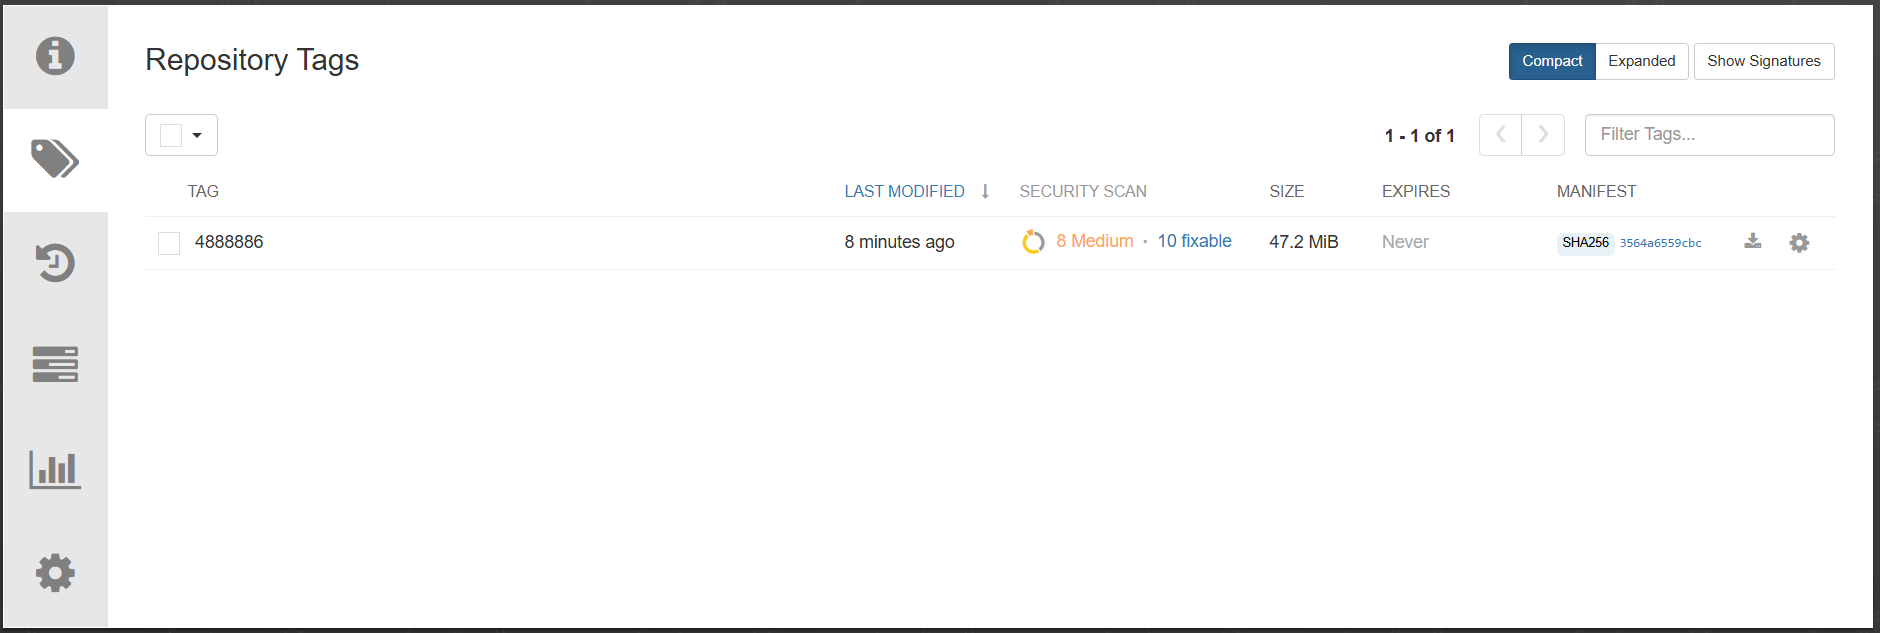
\includegraphics[width=0.90\linewidth]{ci_cd/bloque3_creaccionTag.png}
\caption{Primera imagen publicada en el repositorio \texttt{zelkarrabi/tfm-demo-app} de Quay.io: etiqueta \texttt{4888886} basada en el SHA corto del commit (47.2~MiB)}
\label{fig:ci-primer-tag}
\end{figure}

% ─────────────────────────────────────────────
\section{Análisis de vulnerabilidades: defensa en profundidad con Trivy y Grype}
\label{sec:vuln-analysis}
% ─────────────────────────────────────────────

La incorporación de un segundo motor de análisis de vulnerabilidades no es una decisión de redundancia, sino de complementariedad técnica. Para comprender por qué dos motores son más seguros que uno, es necesario entender las diferencias estructurales entre sus metodologías de análisis y sus fuentes de datos.

\subsection{Arquitecturas de escaneo complementarias}

\textbf{Trivy} \cite{trivy_docs} analiza la imagen directamente, inspeccionando sus capas y extrayendo los paquetes instalados para contrastarlos con su base de datos curada, compuesta por fuentes de Aqua Security y los repositorios de datos de seguridad de las distribuciones Linux (Red Hat Security Advisories, Debian Security Tracker, Alpine SecDB, entre otros). Su fortaleza reside en la cobertura de paquetes del sistema operativo y en la rapidez de su base de datos, que se actualiza con alta frecuencia.

\textbf{Syft + Grype} opera en dos fases. Syft \cite{syft_docs} genera un SBOM de la imagen, que es un inventario estructurado y estandarizado de todos los componentes del artefacto (paquetes del sistema operativo, bibliotecas de lenguaje, binarios). Grype \cite{grype_docs} analiza ese SBOM contra su propia base de datos, que agrega fuentes distintas a las de Trivy: Anchore Enterprise Data, GitHub Security Advisories, National Vulnerability Database (NVD) y fuentes específicas de Python como PyPI Advisory Database. Esta diferencia en las fuentes de datos hace que Grype pueda detectar vulnerabilidades que Trivy no ha incorporado aún en su base de datos, y viceversa.

\subsection{El SBOM como entregable de compliance}

La generación del SBOM mediante Syft no es únicamente un paso intermedio para el análisis con Grype: el fichero producido es un artefacto de \textit{compliance} y trazabilidad con valor propio. Un SBOM documenta, en un formato estructurado y estandarizado, qué componentes forman parte de cada artefacto, con sus versiones exactas y sus licencias. Este inventario permite responder a preguntas de auditoría como: ¿qué versión de \texttt{urllib3} está en producción?, ¿qué artefactos contienen una biblioteca afectada por una CVE recién publicada?

Existen dos estándares principales para la especificación de SBOMs:

\begin{itemize}
  \item \textbf{SPDX} \cite{spdx_spec}: estándar de la Linux Foundation, orientado principalmente a la gestión de licencias de software y al cumplimiento de los requisitos de la cadena de suministro de software del NIST SSDF \cite{nist_ssdf}.
  \item \textbf{CycloneDX} \cite{cyclonedx_spec}: estándar de la OWASP Foundation, orientado específicamente a la seguridad y al ciclo de vida DevSecOps, con soporte nativo para análisis de vulnerabilidades y metadatos de riesgo.
\end{itemize}

El pipeline emite el SBOM en formato \textbf{CycloneDX} (\texttt{-o cyclonedx-json}), el estándar de OWASP orientado a DevSecOps, que Grype consume directamente. El artefacto generado (\texttt{sbom.cyclonedx.json}) se sube al workflow bajo el nombre \texttt{sbom-\$\{SHORT\_SHA\}}, asociándolo al run concreto y a la imagen correspondiente. La Figura~\ref{fig:ci-sbom-upload} muestra la ejecución exitosa del paso \textit{Upload SBOM artifact}: el fichero \texttt{sbom-defe4ef.zip} fue subido con un tamaño final de 490.279~bytes (ID de artefacto \texttt{7196257107}), accesible en la URL de artefactos del workflow \cite{syft_docs}.

\begin{figure}[H]
\centering
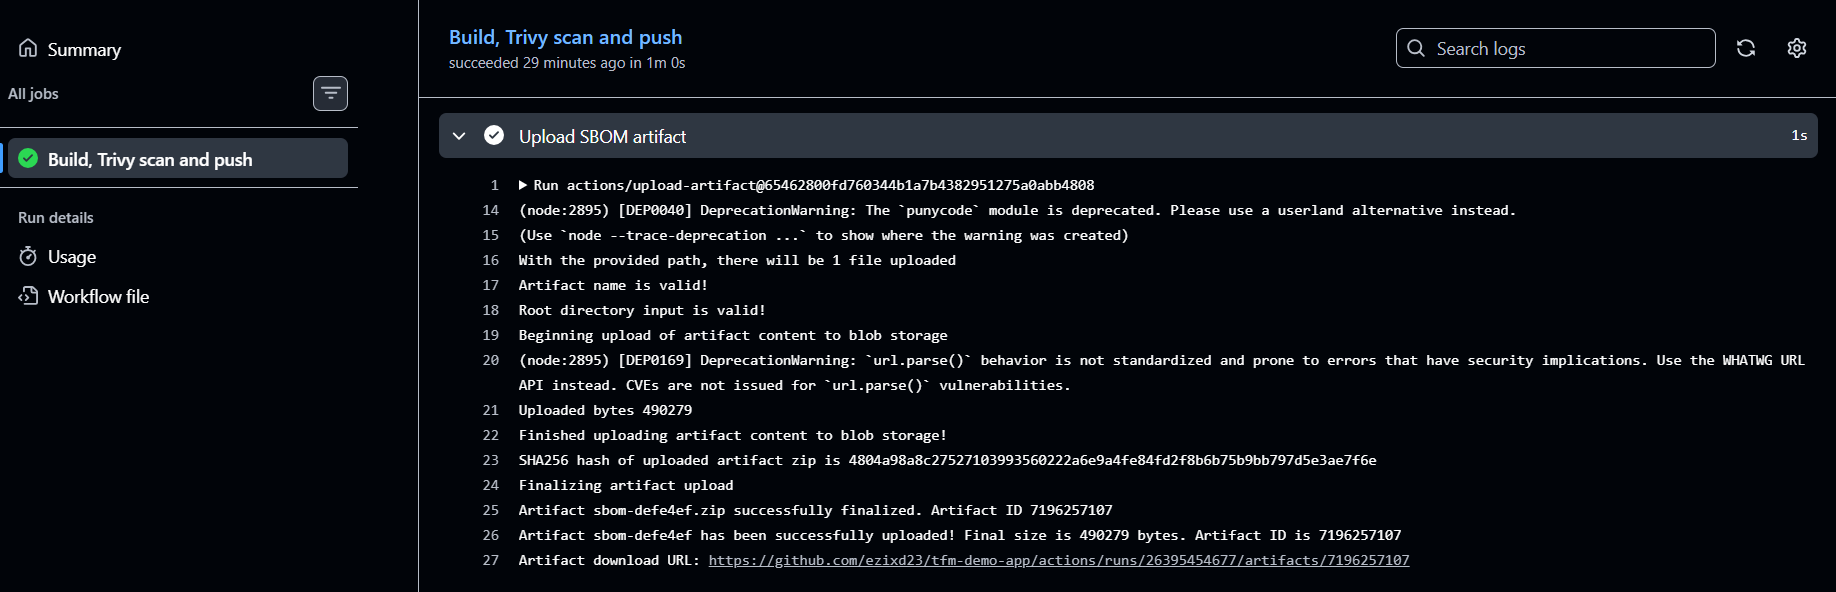
\includegraphics[width=0.95\linewidth]{ci_cd/bloque4_ArtefactoSBOM.png}
\caption{Paso \textit{Upload SBOM artifact}: subida del SBOM \texttt{sbom-defe4ef.zip} como artefacto de auditoría (490.279~bytes, ID~\texttt{7196257107})}
\label{fig:ci-sbom-upload}
\end{figure}

\subsection{Hallazgo empírico: CVE no detectada por Trivy, bloqueante para Grype}

El hallazgo empírico más relevante del capítulo se produjo durante la primera ejecución del pipeline con el doble motor de escaneo activo, utilizando la imagen base \texttt{python:3.12-slim}. Trivy completó su escaneo sin reportar vulnerabilidades por encima del umbral de severidad configurado, y el paso avanzó correctamente. Grype, sin embargo, analizó el SBOM generado por Syft y detectó la vulnerabilidad \textbf{CVE-2025-13836} con severidad \textbf{HIGH} en el binario de Python~3.12.13, con versiones de corrección disponibles a partir de \texttt{3.13.11}, \texttt{3.14.1} y \texttt{3.15.0}. El pipeline falló con código de salida~1 en el paso \textit{Vulnerability scan with Grype}, impidiendo la publicación de la imagen.

La Figura~\ref{fig:ci-grype-output} muestra la salida completa del paso fallido: además de CVE-2025-13836 (HIGH), Grype reportó múltiples vulnerabilidades de severidad MEDIUM en el binario de Python~3.12.13 (CVE-2026-2297, CVE-2026-1299, CVE-2026-0865, CVE-2025-6075, entre otras) y en las dependencias de Python instaladas (\texttt{flask~3.0.3}, \texttt{pip~25.0.1}, \texttt{werkzeug~3.0.4}). La línea de cierre del log, \texttt{Error: Process completed with exit code 1}, confirma que el pipeline se detuvo en este punto, sin ejecutar los pasos de publicación ni de actualización del repositorio GitOps.

\begin{figure}[H]
\centering
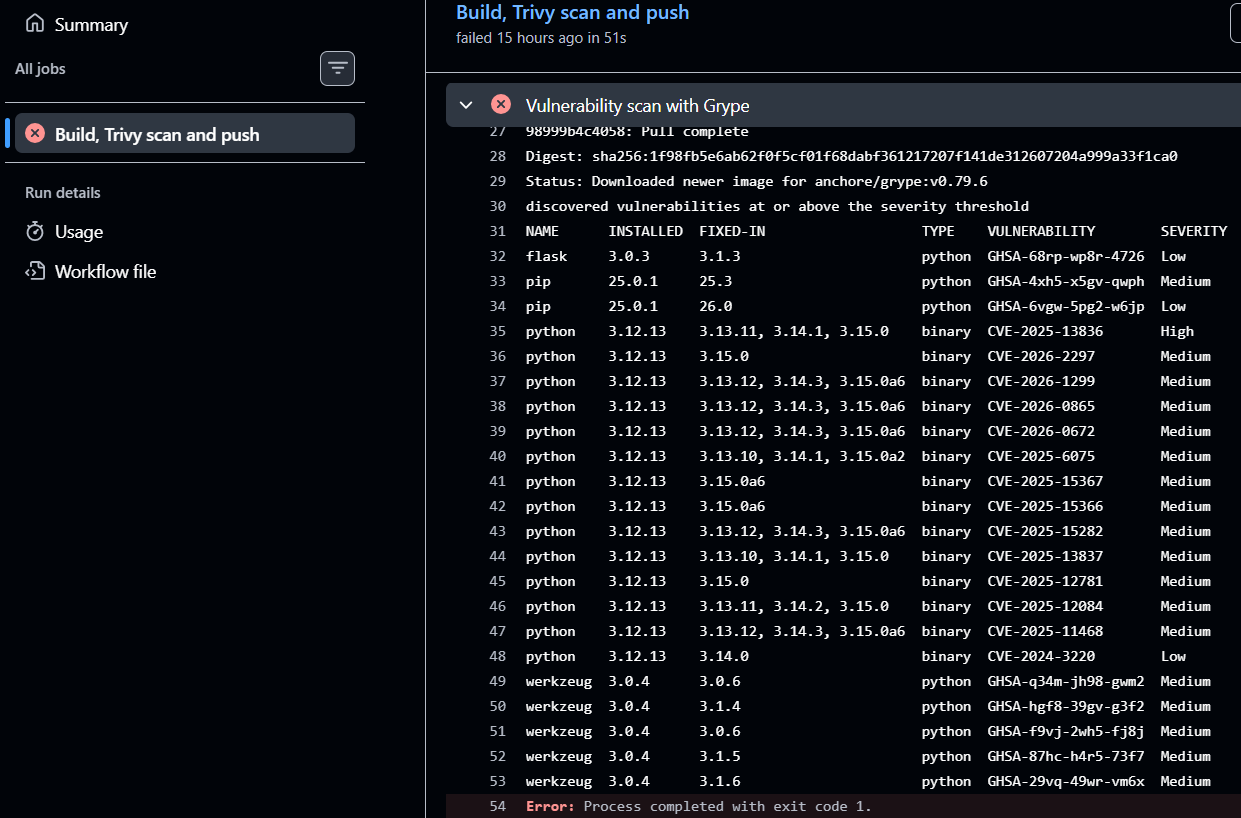
\includegraphics[width=0.95\linewidth]{ci_cd/bloque4_outputTrivyHighPython.png}
\caption{Salida del paso \textit{Vulnerability scan with Grype} (\texttt{anchore/grype:v0.79.6}): bloqueo del pipeline por CVE-2025-13836 (HIGH) en \texttt{python~3.12.13}, con versiones de corrección desde \texttt{3.13.11}}
\label{fig:ci-grype-output}
\end{figure}

Este comportamiento no es un fallo de ninguna de las dos herramientas. Trivy y Grype tienen bases de datos diferentes, taxonomías de severidad distintas y velocidades de incorporación de nuevos CVEs independientes. CVE-2025-13836 estaba presente en la base de datos de Grype en el momento de la ejecución pero no en la de Trivy. Este desfase temporal entre bases de datos es un fenómeno conocido y documentado en la literatura de seguridad de contenedores \cite{nist_sp800190}: las organizaciones que dependen de un único motor de escaneo asumen implícitamente que ese motor tiene cobertura completa de todos los CVEs relevantes, una suposición que este experimento refuta empíricamente.

La conclusión es precisamente la inversa: la diversidad de motores de análisis aporta capas reales de seguridad porque cada motor puede detectar CVEs que los demás no han incorporado aún. El principio de defensa en profundidad, aplicado habitualmente en el plano de controles de acceso y configuración del clúster (Kyverno como motor de admisión, ArgoCD como controlador de estado declarativo), se aplica aquí al plano de la cadena de suministro de imágenes: ningún motor de escaneo es suficiente por sí solo.

Conviene, sin embargo, acotar el alcance del hallazgo. El escaneo en CI es \textit{point-in-time}: solo detecta vulnerabilidades presentes en las bases de datos en el momento del build; una CVE publicada después de que la imagen se haya construido y publicado pasará desapercibida hasta el siguiente ciclo. Esto hace indispensable el re-escaneo periódico de imágenes ya publicadas y la monitorización en tiempo de ejecución ---función que en la arquitectura del Capítulo~5 corresponde a Sysdig. Adicionalmente, la conclusión de defensa en profundidad se apoya en un único caso empírico en el que los motores empleaban taxonomías de severidad distintas; en escenarios donde ambas taxonomías estén alineadas, la diferencia de cobertura entre motores podría ser menor.

% ─────────────────────────────────────────────
\section{Incidencias técnicas y lecciones aprendidas}
% ─────────────────────────────────────────────

Esta sección documenta las tres incidencias técnicas más relevantes surgidas durante la implementación del pipeline. Al igual que las secciones de lecciones aprendidas de los capítulos~6 y~7, el objetivo no es narrar fallos, sino extraer conclusiones técnicas de valor que ilustran principios generales del diseño de sistemas CI/CD seguros.

\subsection{Incidencia 1: ataque de cadena de suministro en la propia action de Trivy}

La primera incidencia afectó al propio mecanismo de defensa diseñado para proteger el pipeline de ataques de cadena de suministro: el anclaje de versiones de actions por SHA. Pese a referenciar \texttt{aquasecurity/trivy-action} mediante su hash SHA completo, el pipeline falló en el primer intento de ejecución con un error de resolución de la action.

La causa raíz, identificada tras analizar los logs del runner, fue que \texttt{aquasecurity/trivy-action} tiene una dependencia transitiva interna hacia una action auxiliar denominada \texttt{setup-trivy}, referenciada mediante una etiqueta mutable (no fijada por SHA). Aqua Security había eliminado o reubicado esta etiqueta como parte de una respuesta a un incidente de seguridad en su propia infraestructura, lo que rompió la cadena de resolución de la action pese a que el SHA de la action principal permanecía intacto.

La Figura~\ref{fig:ci-workflow-inicial} muestra el historial de las dos primeras ejecuciones del workflow: la primera (\textit{feat: initial application code, Dockerfiles and CI workflow}, commit \texttt{6070383}) falló en 7~s por este motivo; la segunda (\textit{ci: update trivy-action SHA to fix broken transitive dependency}, commit \texttt{4888886}) tuvo éxito en 52~s tras actualizar al SHA correspondiente a la versión estable \texttt{v0.35.0}.

\begin{figure}[H]
\centering
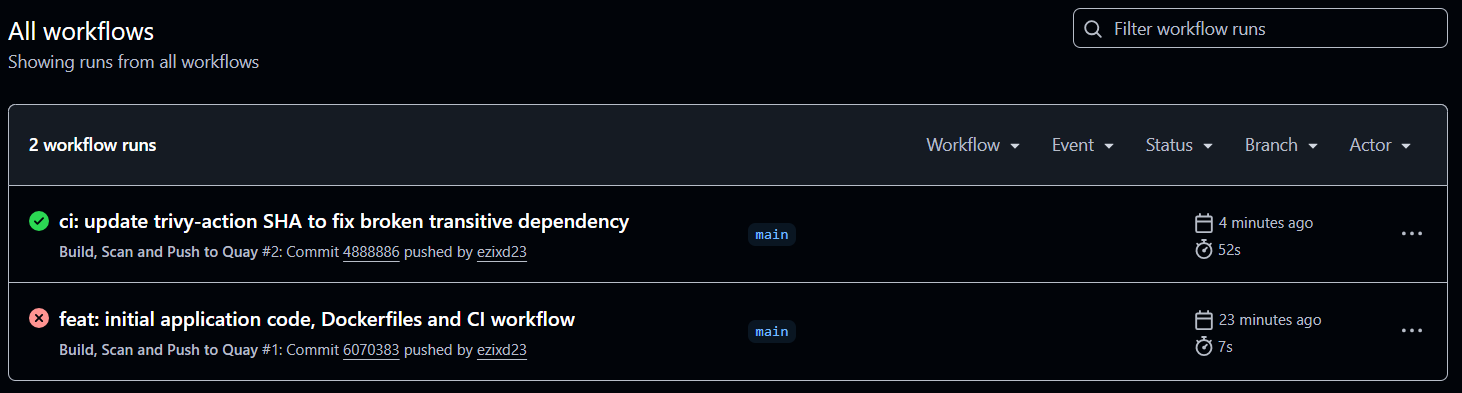
\includegraphics[width=0.95\linewidth]{ci_cd/bloque3_workflowActions.png}
\caption{Historial inicial del workflow: fallo del run~\#1 (7~s) por dependencia transitiva rota en la \textit{action} de Trivy, y corrección en el run~\#2 (52~s) con el SHA de \texttt{v0.35.0}}
\label{fig:ci-workflow-inicial}
\end{figure}

Esta incidencia demuestra empíricamente una limitación real de la seguridad de la cadena de suministro en sistemas de CI basados en componentes de terceros: el anclaje por SHA protege únicamente frente a la mutación del código de la action referenciada directamente, pero no frente a las dependencias transitivas que esa action pueda resolver internamente mediante etiquetas mutables. En un entorno de producción, la mitigación completa requeriría o bien que los proveedores de actions anclen también sus dependencias internas por SHA, o bien el uso de un sistema de \textit{vendoring} que internalice todas las dependencias en el repositorio corporativo. La solución pragmática adoptada ---actualización al SHA de la versión estable con soporte activo--- es un compromiso aceptable que restaura la inmutabilidad del pipeline para la versión más reciente de la action.

\subsection{Incidencia 2: reproducibilidad frente a frescura en la base de datos de Grype}

La segunda incidencia afectó al paso \textit{Vulnerability scan with Grype} tras la incorporación del SBOM. Al fijar la versión de la imagen de Grype como \texttt{anchore/grype:v0.79.6}, la base de datos de vulnerabilidades incluida en esa imagen era estática y databa de la fecha de publicación de la imagen. Por defecto, Grype valida que su base de datos de CVEs no tenga más de 5~días de antigüedad; si el umbral se supera, Grype falla con un error antes de procesar el SBOM.

Este comportamiento expone un \textit{trade-off} fundamental en el diseño de pipelines de seguridad: la \textbf{reproducibilidad} (versión fijada de la imagen, comportamiento determinístico del pipeline) entra en conflicto con la \textbf{frescura} (base de datos de CVEs actualizada, cobertura de las vulnerabilidades más recientes). Priorizar la reproducibilidad implica que el pipeline usará siempre la misma versión de Grype con la misma base de datos, pero esa base de datos se vuelve obsoleta con el tiempo. Priorizar la frescura implica que la imagen de Grype se actualiza automáticamente, pero introduce variabilidad en el comportamiento del pipeline (una ejecución puede fallar no porque la imagen tenga nuevas vulnerabilidades, sino porque la base de datos actualizada incorpora nuevas entradas).

La solución adoptada fue configurar la variable de entorno \texttt{GRYPE\_DB\_VALIDATE\_AGE=false}, que instruye a Grype para que omita la validación de antigüedad y utilice la base de datos disponible en la imagen fijada:

\begin{lstlisting}
- name: Vulnerability scan with Grype
  run: |
    docker run --rm \
      -e GRYPE_DB_VALIDATE_AGE=false \
      -v "$PWD":/work \
      anchore/grype:v0.79.6 \
      sbom:/work/sbom.cyclonedx.json \
      --fail-on high \
      --only-fixed
\end{lstlisting}

Esta decisión prioriza el determinismo del pipeline: el mismo workflow con los mismos inputs producirá siempre el mismo comportamiento, facilitando la depuración de incidencias y la reproducción de resultados. En un entorno productivo, la alternativa recomendada sería una renovación controlada y periódica de la versión de la imagen de Grype mediante un proceso de actualización gestionado (pull request automático semanal, por ejemplo), que combina la actualización de la base de datos con una revisión explícita antes de ser incorporada al pipeline.

La Figura~\ref{fig:ci-workflow-sbom-iteraciones} documenta el historial completo de ejecuciones del workflow durante la resolución de esta incidencia: los runs \#3, \#4 y \#5 corresponden a los intentos de resolución del problema de la base de datos de Grype, hasta alcanzar la solución estable con \texttt{GRYPE\_DB\_VALIDATE\_AGE=false} en el run \#6.

\begin{figure}[H]
\centering
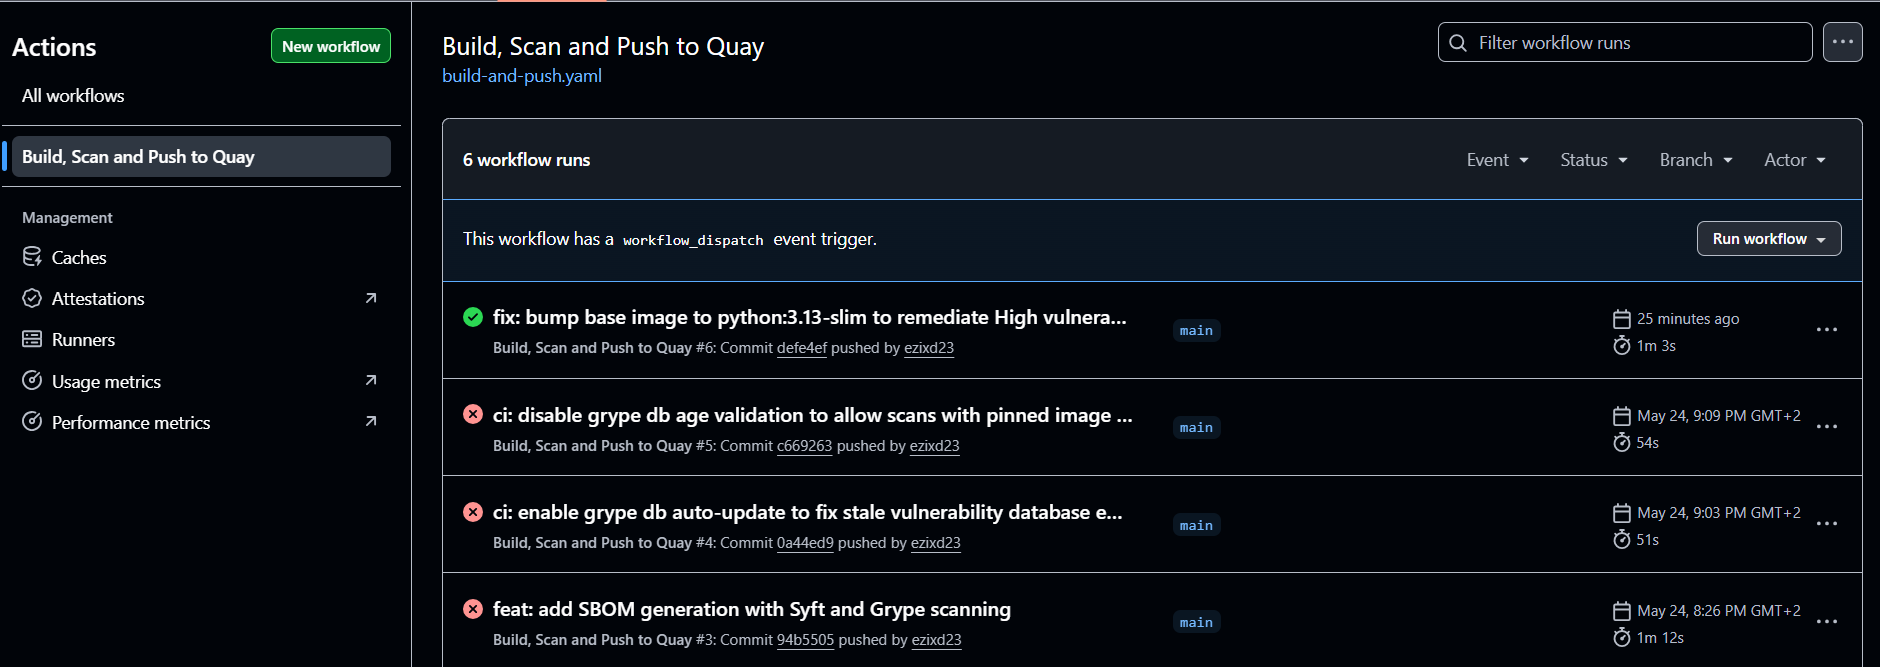
\includegraphics[width=0.95\linewidth]{ci_cd/bloque4_flujoWorkflowAlIncluirSBOMGrype.png}
\caption{Historial del workflow \textit{Build, Scan and Push to Quay}: iteraciones de resolución de incidencias con SBOM y Grype (runs \#3--\#5 fallidos) y ejecución final exitosa con \texttt{python:3.13-slim} (run \#6, commit \texttt{defe4ef})}
\label{fig:ci-workflow-sbom-iteraciones}
\end{figure}

\subsection{Incidencia 3: aplicación del principio Shift-Left ante CVE-2025-13836}

La tercera incidencia es, en términos de valor académico, la más representativa del capítulo: el pipeline bloqueó la publicación de la imagen \texttt{python:3.12-slim} por la CVE-2025-13836 (HIGH) detectada por Grype, tal como se documentó en la Sección~\ref{sec:vuln-analysis}. Ante este bloqueo, existían dos vías de respuesta:

\begin{enumerate}
  \item Reducir el umbral de severidad de Grype de \texttt{HIGH} a \texttt{CRITICAL}, de modo que CVE-2025-13836 no bloqueara el pipeline.
  \item Corregir la vulnerabilidad en el origen actualizando la imagen base a una versión de Python que no contenga el CVE.
\end{enumerate}

La primera opción fue evaluada y descartada porque comprometería los estándares de seguridad del sistema: una vulnerabilidad de severidad HIGH en el runtime de Python no es un falso positivo ni un riesgo aceptable en el contexto de un entorno DevSecOps, y relajar el umbral de detección equivaldría a ignorar sistemáticamente toda vulnerabilidad que no alcance criticidad máxima. La segunda opción, actualizar la imagen base a \texttt{python:3.13-slim}, resuelve el problema en el origen sin comprometer ningún control.

Esta decisión ejemplifica el principio \textit{Shift-Left} \cite{sharma2020devsecops}: en lugar de gestionar la vulnerabilidad en el plano del despliegue (añadiendo excepciones o relajando controles), se corrige en la fase más temprana posible del ciclo de vida ---la selección de la imagen base del Dockerfile. El pipeline no es solo un detector de vulnerabilidades; es un mecanismo que impone una obligación de corrección en el origen antes de que el artefacto avance en la cadena.

La corrección se realizó mediante el commit \texttt{defe4ef} (\textit{fix: bump base image to python:3.13-slim to remediate High vulnerability}). La imagen resultante, publicada en Quay.io bajo la misma etiqueta, tiene 7~vulnerabilidades de severidad media y 8~corregibles con un tamaño de 46.9~MiB --- una reducción tanto en el número de CVEs como en el tamaño de la imagen, resultado esperado al usar una versión más moderna y parcheada de Python.

\textbf{Nota sobre el Dockerfilevulnerable.} El escenario de bloqueo que el \texttt{Dockerfilevulnerable} (basado en \texttt{python:3.4-alpine}) habría permitido reproducir de forma artificial resultó innecesario: el propio pipeline de desarrollo produjo una prueba contrastada genuina al bloquear legítimamente una imagen que el equipo consideraba segura en ese momento (\texttt{python:3.12-slim}). Esta prueba real tiene mayor valor académico que una artificial porque demuestra el sistema funcionando en un escenario de producción donde las vulnerabilidades emergen sin previo aviso: ni el desarrollador eligió deliberadamente una imagen insegura, ni el bloqueo fue preparado. La CVE estaba presente en la base de datos de Grype, la imagen la contenía, y el pipeline hizo exactamente lo que fue diseñado para hacer.

% ─────────────────────────────────────────────
\section{Cierre del ciclo CI/CD: integración con el repositorio GitOps}
% ─────────────────────────────────────────────

El último bloque del pipeline cierra el ciclo CI/CD conectando el plano de Integración Continua documentado en este capítulo con el plano de Despliegue Continuo implementado en el Capítulo~7. Una vez superados todos los controles de seguridad y publicada la imagen en Quay.io, el pipeline actualiza el repositorio GitOps de forma automática.

\subsection{Actualización automática del repositorio GitOps}

El proceso de actualización se realiza en cuatro pasos consecutivos del workflow:

\textbf{Checkout GitOps repository.} El pipeline hace checkout del repositorio \texttt{tfm-gitops} usando el \texttt{GITOPS\_PAT}:

\begin{lstlisting}
- name: Checkout GitOps repository
  uses: actions/checkout@b4ffde65f46336ab88eb53be808477a3936bae11  # v4.1.1
  with:
    repository: ezixd23/tfm-gitops
    token: ${{ secrets.GITOPS_PAT }}
    path: gitops-repo
    ref: main
\end{lstlisting}

El uso del \texttt{GITOPS\_PAT} en lugar del \texttt{GITHUB\_TOKEN} por defecto es una decisión técnica justificada: el \texttt{GITHUB\_TOKEN} tiene permisos únicamente sobre el repositorio en el que se ejecuta el workflow (\texttt{tfm-demo-app}) y no puede escribir en un repositorio diferente. El \texttt{GITOPS\_PAT} es el mecanismo necesario para la escritura cruzada; en producción debería ser un fine-grained PAT limitado a \texttt{tfm-gitops} con \texttt{Contents: read/write}, tal como se razona en la Sección~8.2.

\textbf{Install yq.} Se instala \texttt{yq}, el procesador YAML de línea de comandos de Mike Farah, que permite modificar campos específicos de un fichero YAML sin alterar la estructura del resto del fichero.

La elección de \texttt{yq} frente a alternativas como \texttt{sed} responde a consideraciones de robustez. \texttt{sed} opera sobre texto plano sin comprensión de la estructura YAML: un cambio de formato en el fichero (espaciado diferente, comentarios, reordenación de campos) puede romper la expresión regular de sustitución silenciosamente, produciendo un manifiesto malformado. \texttt{yq}, al procesar el YAML como un árbol de datos estructurado, garantiza que únicamente el campo \texttt{image} del primer contenedor del Deployment es modificado, preservando el resto del fichero sin cambios.

\textbf{Update image tag in GitOps repo.} La actualización del manifiesto se realiza con una expresión \texttt{yq} que navega la estructura del Deployment:

\begin{lstlisting}
- name: Update image tag in GitOps repo
  run: |
    cd gitops-repo
    yq eval -i \
      ".spec.template.spec.containers[0].image = \"${{ steps.vars.outputs.FULL_IMAGE }}\"" \
      applications/demo-app/deployment.yaml
\end{lstlisting}

\textbf{Commit and push to GitOps repo.} El commit incluye un mensaje con trazabilidad cruzada entre repositorios:

\begin{lstlisting}
- name: Commit and push to GitOps repo
  run: |
    cd gitops-repo
    git config user.name "GitHub Actions CI"
    git config user.email "actions@github.com"
    git add applications/demo-app/deployment.yaml
    git commit -m "chore: update demo-app image to ${{ steps.vars.outputs.SHORT_SHA }}"
    git push origin main
\end{lstlisting}

El mensaje de commit incluye el SHA corto de la imagen (\texttt{steps.vars.outputs.SHORT\_SHA}), lo que permite auditar bidireccionalmente: dado un commit en \texttt{tfm-gitops}, es posible identificar la etiqueta de imagen desplegada, y dado un tag de imagen en Quay.io, es posible localizar el commit de código fuente que lo originó.

\subsection{Evidencia empírica del ciclo completo}

La Figura~\ref{fig:ci-git-log} muestra el historial de commits en el repositorio \texttt{tfm-gitops} tras la ejecución del pipeline completo. El commit más reciente (\texttt{f762c09}, \texttt{HEAD}) tiene el mensaje \texttt{chore: update demo-app image to d8ae0bd}, evidencia directa de que el pipeline actualizó automáticamente el repositorio GitOps con la nueva etiqueta de imagen.

\begin{figure}[H]
\centering
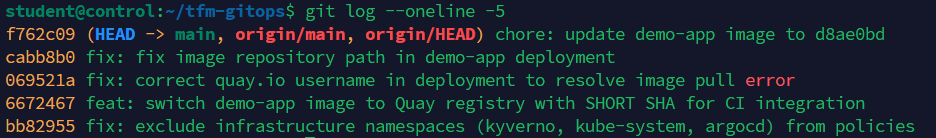
\includegraphics[width=0.90\linewidth]{ci_cd/bloque5_logDeCommitAutomatico.png}
\caption{Historial de commits en \texttt{tfm-gitops}: el commit automático \texttt{f762c09} actualiza la etiqueta de imagen a \texttt{d8ae0bd}, disparando la sincronización de ArgoCD}
\label{fig:ci-git-log}
\end{figure}

Una vez detectado este nuevo commit por ArgoCD mediante su mecanismo de \textit{polling} del repositorio (y su \textit{watch} continuo sobre los recursos del clúster descrito en la Sección~7.5.1), el controlador de reconciliación inicia la sincronización del Deployment con la nueva especificación de imagen. La Figura~\ref{fig:ci-quay-tags} muestra el estado final del repositorio de imágenes en Quay.io, con las dos etiquetas publicadas por el pipeline: \texttt{defe4ef} (imagen con \texttt{python:3.13-slim}, 46.9~MiB) y \texttt{4888886} (imagen intermedia con \texttt{python:3.12-slim}, 47.2~MiB).

\begin{figure}[H]
\centering
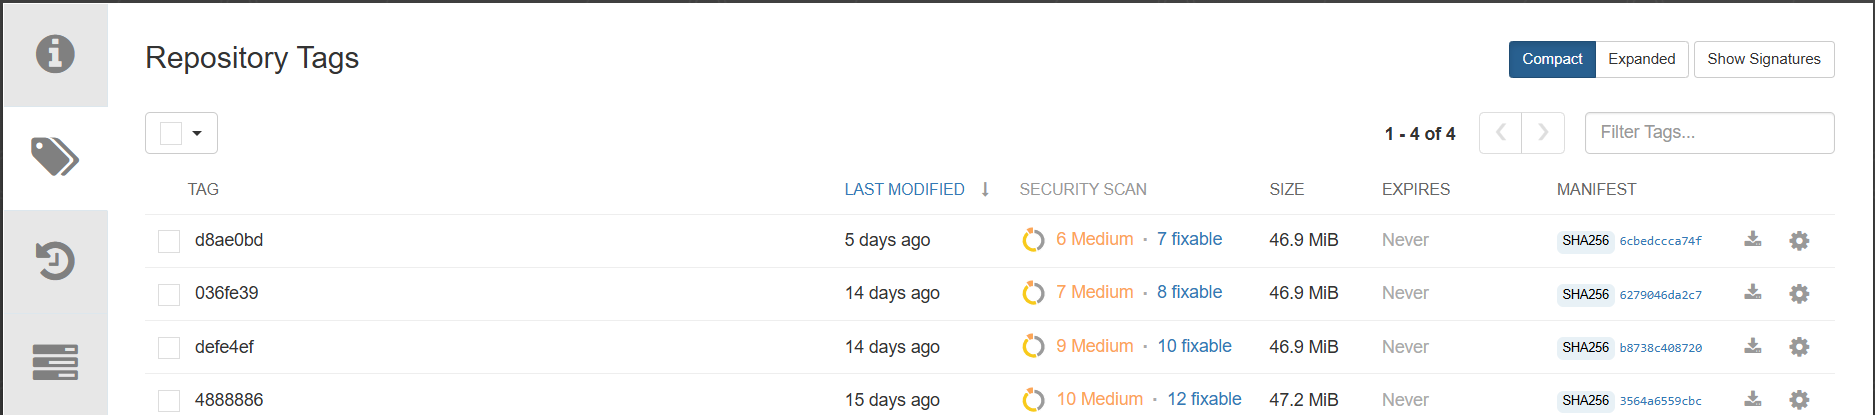
\includegraphics[width=0.95\linewidth]{ci_cd/bloque4_nuevoTAG.png}
\caption{Repositorio \texttt{zelkarrabi/tfm-demo-app} en Quay.io: etiqueta \texttt{defe4ef} (imagen final con \texttt{python:3.13-slim}, 46.9~MiB) y etiqueta \texttt{4888886} (imagen previa con \texttt{python:3.12-slim})}
\label{fig:ci-quay-tags}
\end{figure}

La Figura~\ref{fig:ci-pod-image} muestra la verificación final desde el clúster: los dos pods del Deployment \texttt{demo-app} en estado \texttt{Running} están ejecutando la imagen \texttt{quay.io/zelkarrabi/tfm-demo-app:d8ae0bd}, la etiqueta basada en el SHA corto del último commit que pasó todos los controles del pipeline.

\begin{figure}[H]
\centering
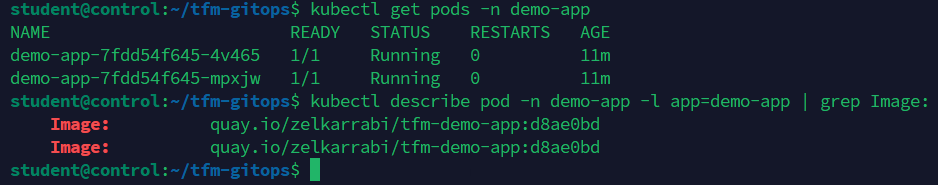
\includegraphics[width=0.90\linewidth]{ci_cd/bloque5_podConImagenActualizada.png}
\caption{Verificación en el clúster: los dos pods de \texttt{demo-app} en estado \texttt{Running} con la imagen \texttt{quay.io/zelkarrabi/\allowbreak{}tfm-demo-app:d8ae0bd} desplegada por ArgoCD}
\label{fig:ci-pod-image}
\end{figure}

La vista del pod en la interfaz de ArgoCD, mostrada en la Figura~\ref{fig:ci-argocd-pod}, presenta el detalle completo del pod \texttt{demo-app-86d6c6d8f7-8s9c6} creado el 06/03/2026 a las 13:45:41: la imagen activa es \texttt{quay.io/zelkarrabi/tfm-demo-app@sha256:6279046da2c79968\ldots}, el estado del contenedor es \texttt{Running} (\textit{started and ready}) y el estado de salud del pod es \texttt{Healthy}. La referencia por digest SHA256 que aparece en el campo \texttt{imageID} del pod no la resuelve ArgoCD: es el kubelet quien, en el momento del pull, descarga la imagen referenciada por etiqueta y registra el digest exacto del manifiesto descargado; ArgoCD únicamente refleja ese valor live desde el estado del pod. El resultado práctico es inmutabilidad efectiva: aunque la etiqueta fuera redirigida en el registro a una imagen diferente, el pod en ejecución ya fijó el digest en su \texttt{imageID}.

\begin{figure}[H]
\centering
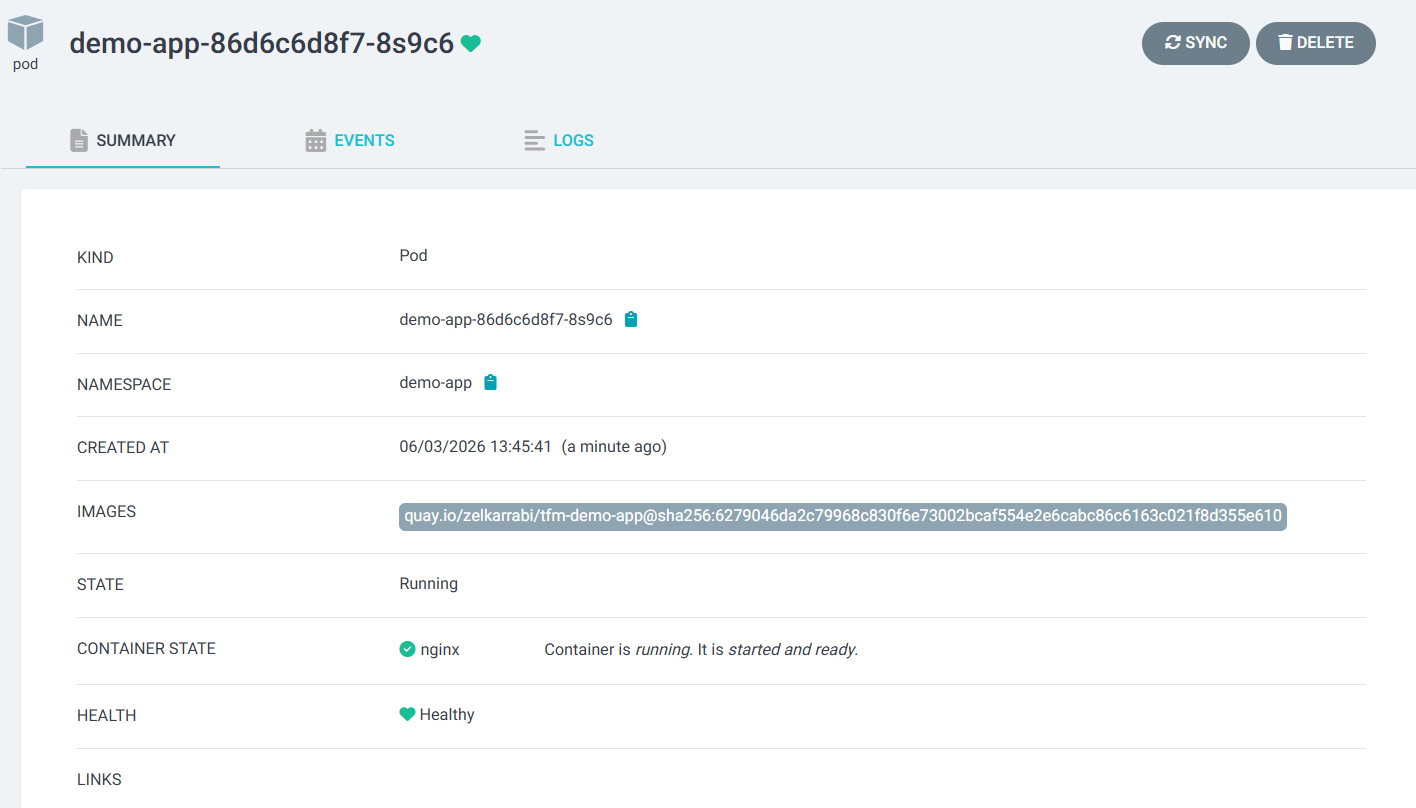
\includegraphics[width=0.85\linewidth]{ci_cd/bloque5_actualizadoImagenQuaypng.png}
\caption{Detalle del pod \texttt{demo-app-86d6c6d8f7-8s9c6} en ArgoCD: imagen activa referenciada por digest SHA256, estado \texttt{Running} y salud \texttt{Healthy}}
\label{fig:ci-argocd-pod}
\end{figure}

La prueba final de extremo a extremo consiste en verificar que el cambio introducido en el código fuente del repositorio \texttt{tfm-demo-app} es visible en la respuesta HTTP de la aplicación desplegada en el clúster. La Figura~\ref{fig:ci-curl-end-to-end} muestra la respuesta de la aplicación accedida en \texttt{192.168.1.101:8888}: el objeto JSON devuelto incluye el campo \texttt{ci\_pipeline:\,"end-to-end-test"}, valor de la variable de entorno \texttt{CI\_PIPELINE} configurada en el Deployment, que confirma que el código desplegado corresponde exactamente al commit que activó el pipeline. El campo \texttt{hostname:\,demo-app-7fdd54f645-4d5nk} identifica el pod específico que atendió la petición, y \texttt{service:\,tfm-demo-app} y \texttt{version:\,1.0.0} corresponden a los valores declarados en el código fuente de la aplicación.

\begin{figure}[H]
\centering
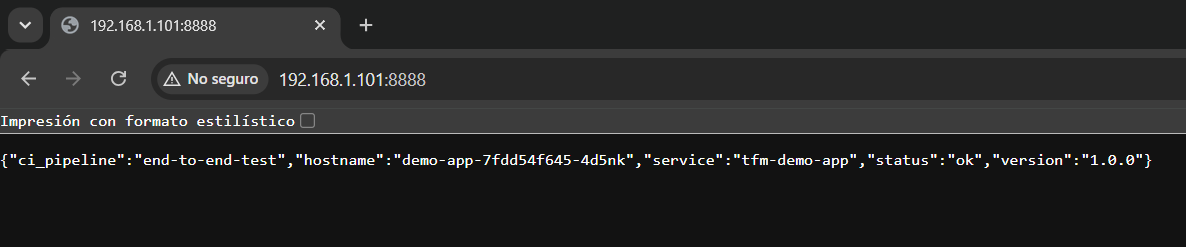
\includegraphics[width=0.80\linewidth]{ci_cd/bloque5_curlMostrandoCambioCodigoFuente.png}
\caption{Respuesta HTTP de la aplicación en \texttt{192.168.1.101:8888}: el campo \texttt{ci\_pipeline:\,end-to-end-test} confirma la propagación completa del cambio de código fuente al entorno de ejecución}
\label{fig:ci-curl-end-to-end}
\end{figure}

\subsection{El ciclo DevSecOps completo}

La combinación de los resultados documentados en este capítulo y en el Capítulo~7 constituye la materialización completa de la arquitectura DevSecOps diseñada en el Capítulo~5. El flujo end-to-end verificado empíricamente es el siguiente:

\begin{enumerate}
  \item Un desarrollador realiza un cambio en el código fuente de \texttt{tfm-demo-app} y hace \texttt{push} a la rama \texttt{main}.
  \item GitHub Actions detecta el evento y lanza el workflow \textit{Build, Scan and Push to Quay}.
  \item El pipeline construye la imagen Docker con el Dockerfile de multi-stage y usuario no root.
  \item Trivy escanea la imagen; si se detecta alguna vulnerabilidad \texttt{HIGH} o \texttt{CRITICAL} con corrección disponible, el pipeline falla aquí.
  \item Syft genera el SBOM de la imagen y lo sube como artefacto permanente de auditoría.
  \item Grype analiza el SBOM; si se detecta alguna vulnerabilidad HIGH o superior, el pipeline falla aquí.
  \item La imagen, libre de vulnerabilidades por encima del umbral, se publica en Quay.io bajo la etiqueta del SHA corto del commit.
  \item El pipeline actualiza el campo \texttt{image} del Deployment en \texttt{tfm-gitops} mediante \texttt{yq} y hace commit con trazabilidad cruzada.
  \item ArgoCD detecta el nuevo commit en \texttt{tfm-gitops} mediante su \textit{watch} sobre los recursos sincronizados y su ciclo de \textit{polling} Git, y sincroniza el Deployment con la nueva imagen.
  \item Kubernetes crea los nuevos pods; Kyverno intercepta la solicitud de creación, aplica las políticas de mutación (P4--P7) y valida contra las políticas de validación (P1--P3, P9). Si el pod no satisface alguna condición no corregible mediante mutación, es rechazado.
  \item Los nuevos pods pasan a estado \texttt{Running} y la aplicación responde HTTP con los valores del nuevo código fuente.
\end{enumerate}

Este flujo integra los tres planos de la arquitectura DevSecOps del Capítulo~5: el plano de desarrollo (código fuente y Git), el plano de automatización (GitHub Actions y ArgoCD) y el plano de ejecución (Kubernetes con Kyverno). La seguridad está integrada en cada transición entre planos: Trivy y Grype entre el plano de desarrollo y el registro de imágenes; las políticas de Kyverno entre el registro y el clúster; y ArgoCD como garante de que el estado del clúster permanece alineado con el repositorio de configuración.

Con el ciclo CI/CD completo implementado y verificado empíricamente, el siguiente capítulo aborda la comparativa práctica entre Kyverno y OPA Gatekeeper, que complementa la revisión teórica del Capítulo~2 con evidencia obtenida mediante la reimplementación directa de un subconjunto representativo de las políticas del Capítulo~6 en el lenguaje Rego de OPA.

\cleardoublepage % Garanteix que la bibliografia comenci en una pàgina imparell
\phantomsection % Marca la pàgina correcta per a la taula de continguts
\addcontentsline{toc}{chapter}{Bibliografia} % Afegeix la bibliografia al ToC
\printbibliography % Imprimeix la bibliografia
\cleardoublepage
\glsaddall
\printglossary
\end{document}